% ------------------------------------------------------------------------
% ------------------------------------------------------------------------
% ICMC: Modelo de Trabalho Acadêmico (tese de doutorado, dissertação de
% mestrado e trabalhos monográficos em geral) em conformidade com 
% ABNT NBR 14724:2011: Informação e documentação - Trabalhos acadêmicos -
% Apresentação
% ------------------------------------------------------------------------
% ------------------------------------------------------------------------

% Opções: 
%   Qualificação          = qualificacao 
%   Curso                 = doutorado/mestrado
%   Situação do trabalho  = pre-defesa/pos-defesa (exceto para qualificação)
%   Versão para impressão = impressao
\documentclass[doutorado, pos-defesa]{packages/icmc}

% ---------------------------------------------------------------------------
% Pacotes Opcionais
% ---------------------------------------------------------------------------
\usepackage{rotating}           % Usado para rotacionar o texto
\usepackage[all,knot,arc,import,poly]{xy}   % Pacote para desenhos gráficos
% Este pacote pode conflitar com outros pacotes gráficos como o ``pictex''
% Então é necessário usar apenas um dos pacotes conflitantes
\newcommand{\VerbL}{0.52\textwidth}
\newcommand{\LatL}{0.42\textwidth}
\let\mathcal\undefined
\DeclareMathAlphabet{\mathcal}{OMS}{cmsy}{m}{n}
% ---------------------------------------------------------------------------
\usepackage{amssymb}% http://ctan.org/pkg/amssymb
\usepackage{pifont}% http://ctan.org/pkg/pifont
\newcommand{\cmark}{\ding{51}}%
\newcommand{\xmark}{\ding{55}}%


% \doublespacing

% \begin{titlepage}
%     \begin{center}
%         {\large \sc UNIVERSIDADE DE SÃO PAULO} \\
%         {\large \sc ESCOLA DE ENGENHARIA DE SÃO CARLOS}\\[0.0cm]
%         {\large \sc DEPARTAMENTO DE ENGENHARIA MECÂNICA}\\[2.0cm]

%         % Título.
%         {
%     \rule{0.9\linewidth}{0.5mm} \\[0.4cm]
%         {\large \bfseries Um estudo sobre Algoritmos de Boosting e a otimização de hiperparametros utilizando Optuna}\\
%         \rule{0.9\linewidth}{0.5mm} \\[7.4cm]
%         {\small \sc  \bfseries{Palavras-chave:}} Gradient Boosting. Aprendizado de
% Máquina Supervisionado. Análise Experimental. Classificação. Otimização. \\[2.0cm]
%         {\small \sc  \emph{Orientador:} Prof.Dr. Marcelo Becker }\\[0.0cm]
%         {\small \sc  \emph{Aluno:} João Manoel Herrera Pinheiro }\\[0.0cm]
%     \end{center}
%     \vfill

%     % Data
%     \begin{center}
%         \makeatletter
%         \@date
%         \makeatother
%     \end{center}
% \end{titlepage}

% \noindent{}
% \newpage
% \setcounter{page}{1}
% \pagestyle{plain}
% ---
% Informações de dados para CAPA e FOLHA DE ROSTO
% ---
% Tanto na capa quanto nas folhas de rosto apenas a primeira letra da primeira palavra (ou nomes próprios) devem estar em letra maiúscula, todas as demais devem ser em letra minúscula.
\tituloPT{Um estudo sobre Algoritmos de Boosting e a Otimização de Hiperparâmetros Utilizando Optuna}
\tituloEN{A Study on Gradient Boosting Algorithms and  Hyperparameter Optimization using Optuna}
\autor[Pinheiro, J. M. H.]{João Manoel Herrera Pinheiro}
\genero{M} % Gênero do autor (M = Masculino / F = Feminino)
\orientador[Orientador]{Prof. Dr.}{Dr. Marcelo Becker}
%\coorientador{Prof. Dr.}{Fulano de Tal}

% \data{07}{02}{2023} % Data do depósito
\idioma{PT} % Idioma principal do documento (PT = português / EN = inglês)
% ---


% ---
% RESUMOS
% ---

% Resumo em PORTUGUÊS
% conter no máximo 500 palavras
% conter no mínimo 1 e no máximo 5 palavras-chave
\textoresumo[brazil]{
    Este trabalho é um estudo sobre os algoritmos de \textit{Gradient Boosting Machines} (GBMs), os quais são  algoritmos de aprendizado de máquina supervisionado que vem obtendo excelente resultados em uma ampla gama de problemas e vencendo diversas competições de aprendizado de máquina. Neste trabalho vamos abordar três bibliotecas que implementam os GBMs, essas bibliotecas são: o XGBoost, CatBoost e LightGBM. Foi realizado um comparativo entre as técnicas e os resultados obtidos, e então partimos para a otimização dos hiperparâmetros utilizando o Optuna. Ao construir um modelo de aprendizado de máquina, a otimização de hiperparâmetros pode se tornar uma tarefa desafiadora e demorada, dependendo do número e do espaço de busca do procedimento de otimização. Definir os hiperparâmetros é uma tarefa fundamental. É necessário entender como eles afetam o resultado do modelo e a partir disso, implementamos o Optuna para os três algoritmos, um framework de otimização de hiperparâmetros. Os conjuntos de dados deste experimento são consumidos da plataforma Kaggle e OpenML. 
    O primeiro experimento realizado foi um comparativo entre os algoritmos pelas métricas de validação e em seguida tentou-se alterar os hiperparâmetros para identificar a influência deles no modelo. Inicialmente, não foi possível obter uma conclusão. Na sequência, foi feita uma análise mais complexa pelo estudo do Optuna. Nesses resultados conseguimos identificar quais hiperparâmetros tiveram seu maior impacto na importância do estudo e se houve alterações desses hiperparâmetros em cada conjunto de dados. 
    Além disso, foi possível melhorar todos os modelos preditivos com apenas a utilização do Optuna. E, ainda, para o modelo com a maior complexidade de previsão, o Optuna demonstrou ser eficaz e resultou em aumento de performance. Com a utilização dos \textit{Shapley Additive exPlanations (SHAP Values)}, conseguimos interpretar os modelos e como cada variável impactou no conjunto de treino.}{Gradient Boosting, Aprendizado de Máquina Supervisionado, Otimização dos Hiperparâmetros, Classificação, Seleção de Modelos, Estudo Empírico, Shapley Values}

% Gradient Boosting. Aprendizado de
% Máquina Supervisionado, Importância de Hiperparâmetros, Otimização dos Hiperparâmetros, Optuna, Análise Experimental, Classificação, Seleção de Modelos, Estudo Empírico

% resumo em INGLÊS
% conter no máximo 500 palavras
% conter no mínimo 1 e no máximo 5 palavras-chave
\textoresumo[english]{
    This thesis is a study about Gradient Boosting Machines (GBMs) algorithms, which are supervised machine learning algorithms that have been getting excellent results on a wide range of problems and winning numerous machine learning competitions. In this work we will approach three libraries that implement the GBMs, these libraries are: XGBoost, CatBoost and LightGBM. A comparison was made between the techniques and the results from each algorithm, and then we started to optimize the hyperparameters using Optuna. When building a machine learning model, hyperparameter optimization can become a challenging and time-consuming task, depending on the number of hyperparameters and the space of the optimization. Defining the hyperparameters is a fundamental task. It is required understand how they affect the result of the model and from that, we implement Optuna, a hyperparameter optimization framework, to the three algorithms. The data sets from this experiment are obtained from the Kaggle and OpenML platform.
    The first experiment was a comparison between the algorithms using validation metrics. Then we attempt to identify the hyperparameters influence on the model by changing their values. Initially, it was not possible to reach a conclusion. Subsequently, a more complex analysis was carried out using Optuna. In these results we were able to identify which hyperparameters had bigger impact on the importance of the study and whether there were changes in these hyperparameters in each data set. Furthermore, it was possible to improve all predictive models with only the use of Optuna. And yet, for the model with the greatest complexity, Optuna proved to be effective and resulted in increased performance. With the use of Shapley Additive exPlanations (SHAP Values), we were able to interpret the models and how each variable impacted on the training set.}{Gradient Boosting, Supervised Machine Learning, Hyperparameter Optimization, Classification, Model Selection, Empirical Study, Shapley Values.}
    
% ----------------------------------------------------------
% ELEMENTOS PRÉ-TEXTUAIS
% ----------------------------------------------------------

% Inserir a ficha catalográfica


% DEDICATÓRIA / AGRADECIMENTO / EPÍGRAFE
\textodedicatoria*{tex/pre-textual/dedicatoria}
\textoagradecimentos*{tex/pre-textual/agradecimentos}
\textoepigrafe*{tex/pre-textual/epigrafe}

% Inclui a lista de figuras
\incluilistadefiguras

% Inclui a lista de tabelas
\incluilistadetabelas

% % Inclui a lista de quadros
% \incluilistadequadros

% Inclui a lista de algoritmos
\incluilistadealgoritmos

% Inclui a lista de códigos
\incluilistadecodigos

% Inclui a lista de siglas e abreviaturas
\incluilistadesiglas

% Inclui a lista de símbolos
\incluilistadesimbolos

% ----
% Início do documento
% ----
\begin{document}
% ----------------------------------------------------------
% ELEMENTOS TEXTUAIS
% ----------------------------------------------------------
\chapter{Introdução}
\label{chapter:introducao}
% Comando simples para exibir comandos Latex no texto
\newcommand{\comando}[1]{\textbf{$\backslash$#1}}


Técnicas de \textit{Machine Learning} estão sendo utilizadas cada vez mais na indústria e ciência com o principal objetivo de obter informações através dos dados. O aumento do uso dessas técnicas se deve ao volume cada vez maior de dados sendo produzidos, bem como o aumento na performance para processar esses dados e a redução de custos para armazená-los. Os modelos de \textit{machine learning} estão sendo usados em diversas áreas da ciência, desde o diagnóstico de algumas doenças pelo reconhecimento de imagens em laboratórios médicos até o reconhecimento de padrões e comportamentos com o objetivo de mapear consumidores e facilitar a tomada de decisão para a venda ou recomendação de algum produto. Com esse forte crescimento, a pesquisa na área teórica e na aplicação de técnicas de \textit{machine learning} vem se se destacando, mostrando a importância de um modelo robusto de \textit{machine learning} para as aplicações científica e industrial.

\textit{Gradient Boosting Machines} (GBMs) vem obtendo resultados no estado da arte, principalmente em casos de dados estruturados, ou seja, dados que possuem um padrão bem definido. Por exemplo: dados organizados através de linhas e colunas, onde não é permitido dados diferentes das estruturas preestabelecidas. Se a coluna de uma tabela foi criada para ser numérica, ela não aceitará outro tipo de dados. Em uma pesquisa feita pela plataforma Kaggle,\textit{State of Data Science and Machine Learning 2022} \cite{kaggle}, GBMs como XGBoost, LightGBM e CatBoost estão entre os algoritmos mais utilizado pelos respondentes da pesquisa. Esses algoritmos são baseados em árvore de decisão e utilizam uma estrutura de \textit{Gradient boosting} para aumentar a performance do modelo.

Além da escolha do melhor algoritmo para construir o seu modelo de \textit{Machine Learning} temos o desafio de escolher os hiperparâmetros para o treino do modelo. Eles são de extrema importância pois são atributos que controlam o treinamento do modelo de \textit{machine learning}. Eles previnem o modelo de aprender apenas com os dados mostrados,  ou seja, previnem \textit{overfitting} e \textit{underfitting}, tornando-o capaz de generalizar para outras situações possíveis. Nas implementações mencionadas -- XGboost, LightGBM e CatBoost -- todos os hiperparâmetros costumam ter valores pré-estabelecidos. Encontrar os melhores hiperparâmetros é uma tarefa extremamente desafiadora na área de \textit{Machine Learning}. Após o comparativo dos modelos de \textit{boosting}, o melhor modelo será escolhido para utilizar uma ferramenta de automatização de hiperparâmetros, o Optuna. Assim, podemos avaliar se apenas o ajuste dos hiperparâmetros é capaz de melhorar o resultado do modelo treinado.

Neste capítulo será abordada a revisão bibliográfica sobre o tema aprendizado de máquina e o embasamento teórico do problema de classificação. Também serão apresentadas as características do conjunto de dados, explicando o conceito de cada variável e a distinção entre variáveis explicativas e variável resposta.

\section{Conceitos Iniciais}
Diversos autores definem aprendizagem como a capacidade de um programa computacional conseguir melhorar seu desempenho através do aprendizado \cite{hastie} \cite{mitchell}, tornando suas ações mais precisas \cite{marsland} ou inferir regras gerais através da observação de exemplos \cite{luxburg:artigo}. Ou seja, a partir de algoritmos de aprendizagem  o computador consegue aprender tarefas específicas. O conceito chave para as máquinas é essa aprendizagem a partir dos dados e que com isso a máquina consiga generalizar, definida como a identificação
de similaridade entre diferentes situações, é o que torna a aprendizagem útil, pois o conhecimento adquirido pode ser aplicado em diversos cenários. 

\subsection{Aprendizado de Máquina}
O aprendizado de máquina mescla ideias da matemática, física, neurociência e biologia. Segundo estes autores, o aprendizado de máquina, diferente da inteligência artificial, não procura gerar um comportamento inteligente, mas descobrir mecanismos através dos quais tarefas específicas podem ser aprendidas por computadores, ou seja com o foco na capacidade de generalização \cite{hastie} \cite{marsland}.
O aprendizado de máquina tem origens na estatística, ciência da computação e inteligencia artificial e agora estabeleceu-se como uma disciplina por direito próprio \cite{luxburg:artigo}.

De maneira geral os problemas de aprendizado podem ser classificados como:
\begin{itemize}
  \item \textbf{Aprendizado Supervisionado:} um conjunto de respostas corretas é fornecido para esse aprendizado de tal forma que o algoritmo escolhido consiga generalizar para responder corretamente as possíveis novas entradas. Alguns algoritimos são ,por exemplo, regressão linear, análise de regressão logística, \textit{K-Nearest Neighbors}, S\textit{upport Vector Machines}, \textit{Random Forests} e Árvores de Decisão.
  \item \textbf{Aprendizado Não Supervisionado:} o conjunto de respostas corretas não é fornecido para o algoritmo e, portando, o algoritmo procura identificar padrões ou similaridades entre os objetos de entrada para que eles apresentem algo em comum e que seja possível agrupá-los. Nesse aprendizado, busca-se encontrar o padrão entre as diferentes amostras e separar as que possuem as mesmas características. Um exemplo desse aprendizado são os algorítimos de clusterização que tem como objetivo agrupamento dos dados que possuem características semelhantes, por exemplo, \textit{K-Means}, DBSCAN e \textit{Hierarchical Cluster Analysis} (HCA). 
  \item \textbf{Aprendizado Por Reforço:} O sistema de aprendizado, que nesse contexto receberá o nome de agente, é treinado para tomar uma sequência de decisões. Nesse tipo de aprendizado o agente executa alguma ação e recebe recompensas ou penalidades em troca. Seu objetivo é ser capaz de tomar as melhores decisões para obter o maior número de recompensas ao longo do tempo, usando testes totalmente aleatórios no início e obtendo a melhor solução ao final. Diferente dos outros, este aprendizado não precisa de dados rotulados para tomar a sua ação. Alguns algoritmos são, por exemplo, Processo de Decisão de Markov, \textit{Q-Learning}, Monte Carlo, \textit{Deep Q-Learning} e \textit{Deep Deterministic Policy Gradient}.
\end{itemize}
\subsection{Problema de Classificação}
Em um problema de classificação temos dois tipos de espaço para ser considerado, conforme abordado em \cite{luxburg:artigo}, temos o espaço $X$ das instancias ou objetos e o espaço $Y$ das saídas ou categorias. No caso que será abordado neste trablaho, a classificação binária, o espaço de saídas é um indicador booleano dado pelo conjunto ${(0,+1)}$  -- em alguns casos podemos ter o conjunto ${(-1,+1)}$. O objetivo é encontrar um mapeamento $f:X \rightarrow Y$ chamado de classificador. Um algoritmo de classificação, portanto, é um procedimento que toma como entrada os exemplos de treinamento e produz como saída um classificador $f$. Este tópico será abordado com maiores detalhes no Capítulo \ref{chapter:fundamentos-aprendizado}.

De maneira geral, os tópicos que descrevem os processos para resolver um problema de aprendizado supervisionado se resumem em \cite{hastie} \cite{marsland}:

\begin{enumerate}
\item \textbf{Coleta e preparação dos dados:} os dados precisam ser coletados e tratados antes de colocar no treino do modelo. É preciso fazer uma análise estatística do conjunto de dados e realizar os tratamentos necessários para os dados faltantes e/ou \textit{outliers}.
\item \textbf{Seleção de variáveis:} requer o conhecimento prévio do problema e dos dados coletados para identificar quais variáveis podem ser úteis para resolver o problema e, se necessário, criar novas variáveis a partir das existentes ou até aplicar redução de dimensionalidade nas variáveis.
\item \textbf{Escolha do algoritmo:} definidos o problema e o conjunto de dados, um ou mais algoritmos de aprendizado de máquina são selecionados.
\item \textbf{Determinação dos parâmetros:} alguns algoritmos necessitam que alguns parametros sejam colocados manualmente, por exemplo, número de interações, tolerância ao erro, tamanho da amostra, etc.
\item \textbf{Determinação dos Hiperparâmetros:} são parâmetros que definem a arquitetura de um método de aprendizado. Enquanto os parâmetros do modelo especificam como transformar os objetos de entrada na saída desejada, os hiperparâmetros definem como o modelo é realmente estruturado. Os hiperparâmetros não podem ser estimados diretamente do conjunto de treinamento. Alguns exemplos de hiperparâmetros são taxa de aprendizado, número de épocas, número de galhos e folhas em uma árvore de decisão, profundidade máxima da folha, etc.
\item \textbf{Treinamento:} com os dados e os algorítimos essa etapa consiste no uso computacional a fim de construir uma função $\hat{f}(x)$ que tem como objetivo prever as saídas a partir de novos dados.
\item \textbf{Validação:} esta etapa inclui a seleção de métricas para avaliação de desempenho do modelo construído, neste caso um classificador. São utilizados dados que não foram usados no conjunto de treinamento do modelo.
\item \textbf{Tuning do Modelo:} esta etapa consiste em melhorar a performance do modelo apenas alterando os parâmetros e/ou hiperparâmetros. É um processo complexo que é utilizado para melhorar a performance dos modelos treinados. Consiste em realizar diversos treinos alterando os hiperparâmetros de forma sistemática e, no final, escolher o modelo com a melhor métrica de performance.
\item \textbf{Predições:} com o modelo finalizado, fazer as predições significa fornecer a ele dados novos e obter as saídas. Essa é a última etapa da resolução de um problema de aprendizado supervisionado, onde podemos concluir que o problema foi resolvido. 
\end{enumerate}
\subsection{Variáveis e Conjunto de Dados}
O conjunto de dados é representado por um vetor de características que descreve as observações. As variáveis são mensuradas em cada elemento da amostra ou população que apresentam características diferentes de indíviduo para indivíduo. 
Quando qualquer medição de uma caracteristica está ausente, dizemos que aquele valor é \textit{missing}. Cada observação, também denominada objeto ou registro, corresponde a uma ocorrência dos dados e cada variável está associada a uma propriedade específica dos objetos, podendo esta propriedade retratar noções físicas ou abstratas. Uma coleção de observações assim constituídas compõe um conjunto de dados. 
As variáveis podem assumir valores numéricos e não numéricos, podemos classifica-las em:

\begin{itemize}
    \item \textbf{Numéricas ou quantitativas:}
    \begin{enumerate}
        \item \textbf{Contínuas:} são variáveis mensuráveis que se originam de algum processo de medição e que podem assumir qualquer valor em uma escala contínua seja $x_i$\simbolo{x_i}{o exemplo i-enésimo de um conjunto de dados, vetor ou escalar} para uma variável contínua temos que $x_i\in\mathbb{R}$ \simbolo{\mathbb{R}}{Conjunto dos números reais}.Exemplos: salário, pressão arterial, altura e etc.
        \item \textbf{Discretas:} são variáveis que são originadas de um processo de contagem, que podem assumir um número finito ou infinito contável de valores. Seja $x_i$ uma variável discreta, temos que $x_i\in\mathbb{Z}$\simbolo{\mathbb{Z}}{Conjunto dos números inteiros}. Exemplos: número de filhos, quantidade de quartos em uma casa e etc.
    \end{enumerate}
    \item \textbf{Categóricas ou qualitativas:}
        \begin{enumerate}
        \item \textbf{Ordinal:} os valores apresentam uma ordem definida e é possível determinar qual é o maior valor e o menor valor. Por exemplo: escolaridade, \textit{rating} de risco de um país, meses do ano, nota de um teste e etc.
        \item \textbf{Nominal:} os valores não apresentam uma ordem definida são penas nomes diferentes que representam alguma característica. Por exemplo: sexo, cor dos olhos, profissão, religião e etc.
    \end{enumerate}
\end{itemize}
Os conjuntos de dados apresentam atributos de entrada, também denominados \textbf{variáveis
explicativas, preditoras ou independentes}, e podem apresentar um atributo alvo, também chamado de \textit{target}, \textbf{variável resposta ou variável dependente}, que representa o evento que queremos realizar as nossas previsões. Nos problemas de regressão, a varíavel resposta contém valores númericos contínuos enquanto que, nos problemas de classificação, o atributo alvo é uma variável discreta, geralmente um indicador booleano $(0,1)$.

Um conjunto de dados é representado por uma matriz de objetos $X_{n\times d}$ em que $n$ é o número de objetos e $d$ é o número de atributos de entrada. Este valor define a dimensão da base de dados e cada elemento $x_{ij}$ da matriz contém o valor da $j$-ésima característica para o $i$-ésmo objeto com $j=1,2,3,...,d$ e $i=1,2,3,...,n$. De maneira análoga, a $i$-ésima observação da variável resposta é representada por $y_i$.
\section{Objetivos}
O principal objetivo desse trabalho é o estudo dos três algorítimos de \textit{boosting} XGboost, LGBM e CatBoost em um problema de classificação binária, comparando a performance e o custo computacional (tempo de execução) de cada algoritmo em diferentes \textit{datasets}. Também é feita uma análise dos hiperparâmetros em cada uma das implementações, avaliando como eles afetam o resultado final dos modelos. E por fim, os hiperparâmetros do LGBM são otimizados utilizando o Optuna, um framework Open Source voltado para automatizar a busca pelos melhores hiperparâmetros. Podemos sumarizar o estudo deste trabalho nos seguintes pontos:
\begin{enumerate}
   \item Quais as principais diferenças de cada algoritmo? O conjunto de dados afeta o resultado final em cada algoritmo ? Qual o algoritmo que obteve a melhor performance tanto do ponto de vista computacional e na métrica de validação ?
   \item Como os hiperparâmetros afetam o treino do modelo? 
   \item Como funciona o Optuna? Após a aplicação do Optuna, conseguimos melhorar a métrica de validação do modelo?
\end{enumerate}

\section{Descrições dos Capítulos}
Nos próximos dois capítulos, \autoref{chapter:fundamentos-aprendizado} e \autoref{chapter:algoritmos-boosting} serão introduzidos os fundamentos teóricos para o aprendizado supervisionado, as métricas de validações, os algoritmos de boosting e o que são hiperparâmetros. No \autoref{chapter:desenvolvimento} temos as implementações das funções dos algoritmos e do optuna, de tal forma que o experimento fique replicável e comparável entre os algoritmos. Além disso, discriminamos a estrutura dos testes realizados. No \autoref{chapter:experimental}, temos o resultado dos testes implementados no \autoref{chapter:desenvolvimento}, além de uma análise estatística dos conjuntos de dados utilizados. Buscamos ainda interpretar quais variáveis impactam o modelo. No \autoref{chapter:resultados} será abordada a análise final, comparando os trés algoritmos, suas métricas de validação, de performance e custo computacional. Em seguida, teremos a análise de alguns hiperparâmetros e, por final, o modelo otimizado pelo Optuna e sua performance. Culminamos no \autoref{chapter:conclusao}, onde teremos a conclusão final de todo o trabalho realizado neste estudo, uma análise das limitações do mesmo, bem como sugestões de trabalhos futuros.

Nos apêndices, se encontram os materiais complementares que contém inclusive o Jupyter Notebook, com os códigos implementados. Há também a  referência da página no \textit{GitHub}, onde o código fonte final deste trabalho está disponibilizado. 


\chapter{Fundamentos de Aprendizado Supervisionado}
\label{chapter:fundamentos-aprendizado}
No aprendizado de máquina, distinguimos três tipos de aprendizado: supervisionado, não supervisionado e de reforço. A distinção geralmente é feita pelo feedback o agente recebe.
A aprendizagem supervisionada é a tarefa de aprender uma função a partir de um conjunto de dados
rotulados. Isso significa que os dados consistem em exemplos de treinamento: as entradas e seus valores de saída desejados. O problema pode ser uma classificação, se a saída for uma
classe, ou um regressão, se a saída for um ou vários valores reais. Em ambos os casos, o feedback é
a saída correta que corresponde à entrada fornecida. Um modelo treinado totalmente supervisionado
serve como uma função que podemos usar para mapear novas entradas. O objetivo é ser capaz de
rotular dados novos corretamente: exemplos que não estavam no conjunto de treinamento. 

Em resumo, o principal objetivo de \textit{Machine Learning} é descobrir padrões a partir do conjunto de dados para que se possa obter \textit{insights} e resolver diversos problemas em campos diferentes. Problemas de aprendizado supervisionado lidam especificamente com dados no formato $(\mathbf{x}^{(i)},y^{(i)})$, em que $y^{(i)}\in\mathbb{R}$ é a saída desejada. Ou seja, a saída também está contida no conjunto de dados.

Em \cite{russel} o principal objetivo do aprendizado supervisionado pode ser definido como:

Dado um \textbf{conjunto de treino} com $N$ pares de entrada-saída 
\begin{gather*}
    \{(\mathbf{x}^{(1)},y^{(1)}),(\mathbf{x}^{(2)},y^{(2)}),...,(\mathbf{x}^{(N)},y^{(N)})\}
\end{gather*}

onde cada $y^{(i)}$ foi gerado por uma função desconhecida $y=f(x)$, devemos descobrir uma função $h$ que se aproxima da real função $f$.

A função $h$ é chamada de \textbf{Hipótese} e está contida em um \textbf{Espaço de Hipóteses} denominado de $\mathcal{H}$ ou seja o espaço contem a classe de funções consideradas por um algoritmo de aprendizagem, que irá escolher a função $h \in \mathcal{H}$ baseado em uma função de erro calculada no \textbf{conjunto de treino} em que a saída $y_i$ é o valor que estamos tentando prever com o nosso modelo.

Em seguida, listamos alguns exemplos clássicos de aprendizado supervisionado: Detecção de fraude em cartões de credito em que $\mathbf{x}^{(i)}$ seriam informações da transação (local, valores, forma de pagamento) e o ${y}^{(i)}$ um indicador booleano se a $i$-th é uma transação fraudulenta ou não. Predição de preços de imóveis em que $\mathbf{x}^{(i)}$ seriam informações do imóvel (local, área do imóvel, quantidade de quartos, ano de construção) e o ${y}^{(i)}$ é o valor do imóvel. Classificação de dígitos manuscritos, onde $\mathbf{x}^{(i)}$ é uma imagem ou a
representação de um número e ${y}^{(i)}$ o número correspondente.

\section{Função Aproximação e Otimização}

A tarefa do aprendizado supervisionado pode ser interpretada como um problema de otimização. Conforme abordado em \cite{hastie}, 
temos o paradigma da \textit{function-fitting}. Do ponto de vista de aprendizado de máquina, vamos assumir que os erros são aditivos e que temos o modelo $Y = f(x) + \epsilon$. A aprendizagem supervisionada tenta aprender $f$ por
exemplo através de um \textit{professor}. 

Observa-se o sistema em estudo, tanto
as entradas quanto as saídas, e monta-se um conjunto de treinamento de observações \simbolo{\mathcal{T}}{Conjunto de treino}$\mathcal{T} =
(\mathbf{x}^{(i)},{y}^{(i)}), i = 1, . . . , N$ . Os valores de entrada observados para o sistema $\mathbf{x}^{(i)}$ também são alimentados em um sistema artificial, conhecido como um algoritmo de aprendizagem, que também produz saídas $\hat{f}(x^{(i)})$ em resposta. O algoritmo de aprendizado tem a propriedade de poder modificar sua relação de entrada/saída $\hat{f}$ em resposta às diferenças ${y}^{(i)}-\hat{f}(x^{(i)})$ entre as saídas originais e geradas. Esse processo é conhecido como \textit{aprendizado por exemplo}. Após a conclusão do processo de aprendizagem, o objetivo final é que as saídas artificiais e as saídas reais estejam próximas o suficiente para o modelo consiga generalizar para todos os conjuntos de entradas.

As diferentes funções $\hat{f}$ podem ser estimadas a partir de diferentes modelos em que a hipótese escolhida se aproximará da verdadeira função $f$. Alguns exemplos são estimativa por máxima verossimilhança, o método dos mínimos quadrados, expansões lineares e transformação \textit{sigmoid}.

Para estimar os parâmetros dessas aproximações, os algoritmos de aprendizado geralmente realizam uma otimização sobre uma \textit{função de perda} \cite{kuhn} que depende do aproximador escolhido.

\section{Viés-Variância \textit{Tradeoff}}
O objetivo dos modelos de aprendizado de máquina é estimar a função que melhor ajusta aos dados de entrada para obter previsões corretas de forma generalizada. A melhor maneira de medir e otimizar o desempenho do modelo é levar em consideração o viés e a variância.

O problema básico de aprendizado supervisionado geralmente consiste em dois conjuntos de dados: \textbf{conjunto de treinamento} e
o \textbf{conjunto de teste}. Um modelo é treinado usando dados do conjunto de treinamento, resultando em um modelo $\hat{f}$, então este modelo prevê os dados no conjunto de teste, e com o previsto $\hat{y}^{(i)}$ é possível estimar o erro de previsão do modelo.

Se estivermos em uma situação com bastante volume de dados, a melhor abordagem é dividir aleatoriamente o conjunto de dados em três partes: um conjunto de treinamento, um conjunto de validação e um conjunto de teste. O conjunto de treinamento é usado para ajustar os modelos, a validação é usado para estimar o erro de previsão para a seleção do modelo, o conjunto de teste é utilizado para avaliação do erro do modelo final escolhido.

Idealmente, o conjunto de teste deve ser mantido separado dos outros conjuntos e ser utilizado apenas no final da análise de dados. Suponha que usamos o conjunto de teste repetidamente, escolhendo o modelo com o menor erro desse conjunto, então o  erro definitivo do modelo final escolhido irá subestimar o verdadeiro erro de teste, às vezes substancialmente.
É difícil dar uma regra geral sobre como escolher o número de
observações em cada uma das três partes, pois isso depende do conjunto de dados em si, quantidade de ruído e o tamanho da amostra de treinamento, porém uma divisão típica pode
ser 50\% para treinamento e 25\% cada para validação e teste:

\begin{figure}[htb]
 \caption{Divisão de Treino, Validação e Teste}
 \label{fig:treino_test_split}
 \centering
 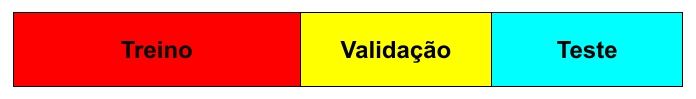
\includegraphics[scale=0.4]{images/treino_teste_split.png}
\end{figure}


O \textit{tradeoff} de viés-variância \cite{hastie} na modelagem preditiva afeta a capacidade de um método de aprendizagem para generalizar. Alta variância indica que o modelo ajusta o ruído aleatório no conjunto de treinamento, o que geralmente resulta em baixo poder de generalização, causando o \textbf{overfitting}. Por outro lado, um modelo com viés alto tem uma diferença muito baixa no erro de previsão entre o conjunto de treinamento e conjunto de teste, mas geralmente tem desempenho ruim causando o \textbf{underfitting}. 

No treinamento e avaliação do modelo, é importante verificar o desempenho da generalização, e isso geralmente é feito usando o conjunto de teste. No processo de avaliação, o \textbf{overfitting} e o \textbf{underfitting} podem ser detectados comparando o erro de previsão no conjunto de treinamento e teste.

A Figura \ref{fig:bias_variance_comp} ilustra uma questão importante na avaliação da capacidade de generalização do modelo. Considere primeiro o caso de um quantitativo ou intervalo resposta de escala. Temos uma variável de resposta $Y$ , um vetor de entradas $\mathbf{X}$ e um modelo de predição $\hat{f}(X)$ que foi estimado a partir de um conjunto de treinamento $\mathcal{T}$ . 

A função para medição do erro entre $Y$ e $\hat{f}(X)$ é denotada por $L(Y,\hat{f}(X))$. Ainda neste Capítulo serão abordadas demais formas para medir o desempenho, mas algumas escolhas típicas para esse erro são:
\begin{equation}
  L(Y,\hat{f}(X)) =
    \begin{cases}
      {(Y - \hat{f}(X))}^2 & \text{erro quadrático}\\
      |Y - \hat{f}(X)| & \text{erro absoluto}
    \end{cases}       
\end{equation}

\begin{figure}[htb]
 \caption{Comportamento das amostra de teste e treino conforme a complexidade do modelo é variada. As curvas em azul claro mostram o erro $\overline{err}$ de treinamento, enquanto o
curvas vermelhas claras mostram o erro de teste condicional $Err_{\mathcal{T}}$ para 100 conjuntos de treinamento de tamanho 50 cada, à medida que a complexidade do modelo aumenta. As curvas sólidas mostram o  erro de teste esperado $Err$ e o erro de treinamento esperado $E[\overline{err}]$ \cite{hastie}
}
 \label{fig:bias_variance_comp}
 \centering
 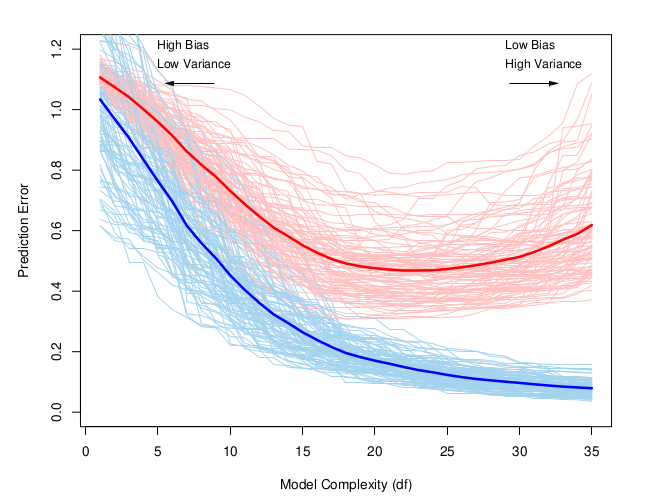
\includegraphics[scale=0.5]{images/bias_viariance.png}
\end{figure}

O erro do teste em uma amostra independente é dado por:

\begin{equation}
    Err_{\mathcal{T}} = E[L(Y,\hat{f}(X))|\mathcal{T}]
\end{equation}

Em que tanto $X$ quanto $Y$ são amostras aleatórias da população. Neste caso, o conjunto de treino $\mathcal{T}$ é fixo e o erro do conjunto de teste é referente a este conjunto de treino fixo $\mathcal{T}$. Podemos escrever esse erro como:
\begin{equation}
    Err = E[L(Y,\hat{f}(X))] = Err_{\mathcal{T}}
\end{equation}

O objetivo é estimar o $Err_{\mathcal{T}}$.

\section{Problema de Classificação}
Conforme foi abordado no Capítulo \ref{chapter:introducao}, quando os valores de $f$ pertencem a um conjunto finito temos um problema de classificação e especialmente quando o valor de $f$ assume apenas dois possíveis valores denotamos de \textbf{classificação binária}.
\begin{figure}[htb]
 \caption{Exemplo de limite de decisão para um classificador binário \cite{hastie}.}
 \label{fig:clas_ex}
 \centering
 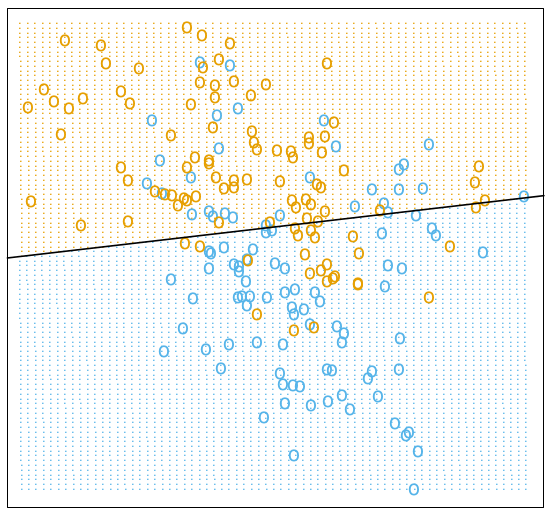
\includegraphics[scale=0.4]{images/classificacao_hastie_ex.png}
\end{figure}

O exemplo de detecção de fraude no cartão de cŕedito que foi abordado no começo deste Capítulo é um problema de classificação bińaria.

\section{Métricas de Avaliação de Performance}
Existem diversas métricas para avaliar a performance de modelos de classificação. Neste estudo as métricas abordadas serão a \textit{AUC}, que é um acrônimo da área em baixo da curva característica de operação do receptor, \textit{Logloss}, que é a perda logarítmica, e o \textit{KS}, que é o Teste Kolmogorov-Smirnov. Um breve resumo de cada métrica:

\begin{itemize}
    \item \textbf{AUC:} é amplamente utilizado em pesquisas, e é uma boa métrica insensível ao desequilíbrio de classes, tendo um valor limitado entre 0.5 e 1.
    \item \textbf{Logloss:} \textit{logloss} é a função direta otimizada nos experimentos, ou seja, as etapas de aumento de gradiente estão tentando reduzir a perda logarítmica em cada etapa. O \textit{logloss} leva em conta a incerteza da previsão e quanto o rótulo real difere dela, tendo seu valor limitado a $]\infty,0]$
    \item \textbf{KS:} o teste Kolgomorov-Smirnov (KS) busca avaliar a distância entre uma distribuição conhecida e uma distribuição que foi observada empiricamente. A hipótese nula do KS é que a amostra segue a mesma distribuição que a normal, tendo o valor limitado entre 0 e 1.
\end{itemize}

\subsection{AUC}

A curva característica de operação do receptor é uma curva de probabilidade que mede a previsão de um classificador binário dado um \textit{threshold}. Os resultados de uma classificação binária podem ser resumidos em uma matriz de confusão, ilustrada na Tabela \ref{tabela:matriz_conf}.Os Verdadeiro-positivo (VP), Falso-positivo (FP), Falso-negativo (FN) e Verdadeiro-negativo (VN) são calculados dispondo todos os dados na matriz, dependendo da classe prevista e da classe real de cada ponto no conjunto de dados.

\begin{table}[htb]
\centering
\caption{Matriz de confusão para o problema de classificação binária.}
\label{tabela:matriz_conf}
\begin{tabular}{|p{3cm}|p{5cm}|p{5cm}|} 
 \hline
\textbf{Resultado} & \multicolumn{2}{c|}{\textbf{Classe Real}} \\
  \hline
  \textbf{Classe Predita} & \textbf{Positivo} & \textbf{Negativo} \\
  \hline
  \textbf{Positivo} & Verdadeiro-positivo (VP) & Falso-positivo (FP) \\
  \hline
  \textbf{Negativo} & Falso-negativo (FN) & Verdadeiro-negativo(VN) \\
  \hline
\end{tabular}
\end{table}

\begin{figure}[htb]
 \caption{Uma ilustração da ocorrência de eventos positivos e negativos
quando ordenado pela variável contínua $y$ \cite{BROWN200624}.}
 \label{fig:roc_brown}
 \centering
 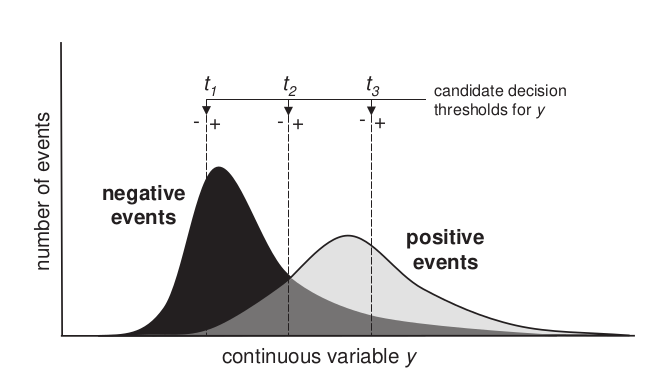
\includegraphics[scale=0.5]{images/roc_threshold.png}
\end{figure}

Conforme abordado em \cite{BROWN200624}, \cite{FAWCETT2006861} e \cite{kuhn} a curva característica do operador (ROC) é calculada pelo gráfico de \textit{Taxa de Verdadeiros Positivos (TVP)}, ou Sensibilidade, versus \textit{Taxa de Falso Positivos (TFP)}, ou Especificidade, onde $\mathcal{T}$ é o \textit{threshold}.

\begin{gather*}
    Roc_{y}(\mathcal{T}) = TVP_{\mathcal{T}} = \frac{VP_{\mathcal{T}}}{VP_{\mathcal{T}} + FN_{\mathcal{T}}} \\
    Roc_{x}(\mathcal{T}) = TFP_{\mathcal{T}} = \frac{FP_{\mathcal{T}}}{FP_{\mathcal{T}} + VN_{\mathcal{T}}}
\end{gather*}

\begin{figure}[H]
 \caption{Curva ROC de um classificador \cite{kuhn}, dois pontos estão em destaques para mostrar diferentes valores de \textit{Especificidade} e \textit{Sensibilidade}}
 \label{fig:roc_kuhn}
 \centering
 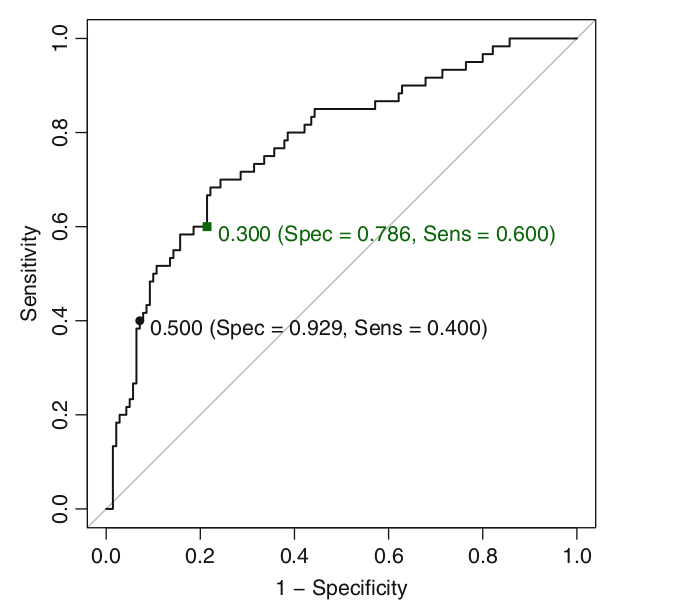
\includegraphics[scale=0.4]{images/roc_kuhn.png}
\end{figure}

Todas as métricas dependem do \textit{threshold} $\mathcal{T}$. A \textbf{AUC} é definida como a área em baixo da curva ROC e fornece uma medida agregada do desempenho do classificador em relação a todos os \textit{threshold} possíveis. O valor é entre 0.5 (pior performance) e 1 (performance perfeita).

Abaixo temos os algoritmos para a geração dos pontos da curva \textbf{ROC} e do cálculo da \textbf{AUC} \cite{FAWCETT2006861}.

\begin{algorithm}[H]
\caption{Algoritmo de geração de curva ROC}\label{algoritmo:roc}
\label{algo:roc}
\textbf{Input:} $L$, o conjunto de exemplos de teste; $f(i)$, o modelo probabilístico
dos classificadores que estimam que o exemplo $i$ é positivo, $P$ e $N$, o
número de exemplos positivos e negativos.\\
\textbf{Output:} $R$, uma lista de pontos ROC aumentando pela taxa FP. \\
\textbf{Requer:} $P>0$ e $N>0$. \\
\begin{algorithmic}[1]
\State $L_{sorted}$ \Comment{$L$ ordenada pelos valores decrescentes de $f$}
\State $FP$ $\leftarrow$ $VP$ $\leftarrow$ $0$ 
\State $R$ $\leftarrow$ [] 
\State $f_{prev}$ $\leftarrow -\infty$ 
\State $i$ $\leftarrow$ $1$
\While{$i\leq |L_{sorted}|$} 
\If{$f(i) \neq f_{prev}$}
\State push $(\frac{FP}{N},\frac{VP}{P})$ onto $R$
\State $f_{prev} \leftarrow f(i)$
\EndIf
\If{$L_{sorted}[i]$ for positivo}
\State $VP \leftarrow VP + 1$
\Else
\State $FP \leftarrow FP + 1$
\EndIf
\State $i \leftarrow i + 1$
\EndWhile
\State push $(\frac{FP}{N},\frac{VP}{P})$ onto $R$
\end{algorithmic}
\end{algorithm}

\begin{algorithm}[H]
\caption{Algoritmo para calcular a área em baixo da curva ROC}\label{algoritmo:auc}
\label{algo:auc}
\textbf{Input:} $L$, o conjunto de exemplos de teste; $f(i)$, o modelo probabilístico
dos classificadores que estimam que o exemplo $i$ é positivo, $P$ e $N$, o
número de exemplos positivos e negativos.\\
\textbf{Output:} $A$, a área em baixo da curva ROC. \\
\textbf{Requer:} $P>0$ e $N>0$. \\
\begin{algorithmic}[1]
\State $L_{sorted}$ \Comment{$L$ ordenada pelos valores decrescentes de $f$}
\State $FP$ $\leftarrow$ $VP$ $\leftarrow$ $0$ 
\State $FP_{prev}$ $\leftarrow$ $VP_{prev}$ $\leftarrow$ $0$ 
\State $A$ $\leftarrow$ $0$
\State $f_{prev}$ $\leftarrow -\infty$ 
\State $i$ $\leftarrow$ $1$
\While{$i\leq |L_{sorted}|$} 
\If{$f(i) \neq f_{prev}$}
\State $A \leftarrow A +$  AREA\_TRAPEZIO($FP,FP_{prev},VP,VP_{prev}$)
\State $f_{prev} \leftarrow f(i)$
\State $FP_{prev} \leftarrow FP$
\State $VP_{prev} \leftarrow VP$
\EndIf
\State $i \leftarrow i + 1$
\If{$i$ for positivo}
\State $VP \leftarrow VP + 1$
\Else
\State $FP \leftarrow FP + 1$
\EndIf
\State $i \leftarrow i + 1$
\EndWhile
\State $A \leftarrow A +$  AREA\_TRAPEZIO($N,FP_{prev},N,VP_{prev}$)
\State $A \leftarrow  \frac{A}{P \times N}$
\Function {AREA\_TRAPEZIO}{$X1,X2,Y1,Y2$}
\State Base $\leftarrow |X1 - X2|$
\State Altura $\leftarrow \frac{Y1+Y2}{2}$
\State \Return Base $\times$ Altura
\EndFunction
\end{algorithmic}
\end{algorithm}

\subsection{Logloss}
Perda Logarítmica ou \textbf{Logloss} é uma função que mede a precisão de um classificador penalizando erros com base na incerteza na previsão, ou seja, verifica se as probabilidades emitidas pelo modelo estão alinhadas com a proporção real de ocorrências do alvo \cite{DBLP:journals/corr/Vovk15}. Nessa métrica, quanto menor o valor melhor: o 0 é a predição perfeita. Conforme veremos no Capítulo \ref{chapter:algoritmos-boosting}, essa é a função de perda que é normalmente otimizada pelos algorítimos de boosting.

A equação da \textit{logloss} para classificadores binários é dada por:
\begin{equation}
    Logloss = -\frac{1}{N}\sum_{i=1}^n[y^{(i)}\log \hat{y}^{(i)} + (1-y^{(i)})\log(1-\hat{y}^{(i)})]
\end{equation}

O gráfico abaixo mostra a faixa de possíveis valores de perda dada uma observação verdadeira (\textit{target} = 1). À medida que a probabilidade prevista se aproxima de 1, a perda de logarítmica diminui lentamente enquanto que à medida que a probabilidade prevista diminui, a perda de logarítmica aumenta rapidamente. A perda de logarítmica penaliza ambos os tipos de erros, mas especialmente aquelas previsões que não são confiáveis.

\begin{figure}[H]
 \caption{\textit{Logloss} em função das predições de uma observação \cite{mlcheat:log}}.
 \label{fig:log_loss_gra}
 \centering
 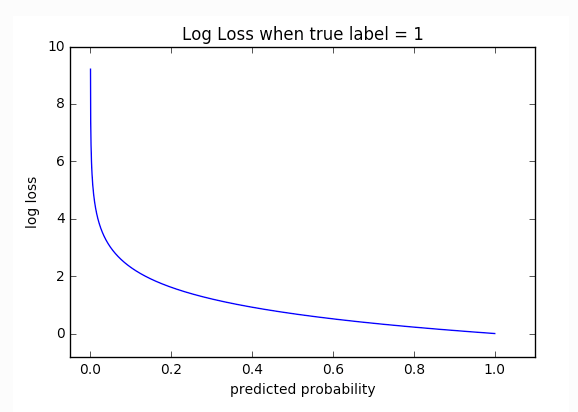
\includegraphics[scale=0.5]{images/logloss_grap.png}
\end{figure}


\subsection{Teste de Kolmogorov-Smirnov}
O Teste de Kolmogorov-Smirnov \cite{kolmogorov,smirnov} também é conhecido como teste de KS ou teste K-S. É um teste de aderência: verifica o grau de concordância entre a distribuição de um conjunto de valores (por exemplo, os escores observados pelo modelo) e alguma distribuição teórica. Esse teste pode ser usado para verificar se os dados seguem, por exemplo, a distribuição normal. A distribuição de frequência acumulada é comparada com a distribuição de frequência observada. A distribuição teórica representa o que seria esperado sobre $H_0$\simbolo{H_0}{Hipótese Nula}, hipótese nula. É determinado o ponto em que as duas distribuições, teórica e observada, tem a maior diferença. \cite{nonparametric}. 

Seja $F_0(X)$ uma função de distribuição de frequências relativas acumuladas, a distribuição teórica sob $H_0$, pra qualquer valor de $X$, o valor de $F_0(X)$  ́e a proporção de casos esperados com escores menores ou iguais a $X$.

Seja $\hat{F}_n$ a distribuição de frequências relativas acumuladas observada de uma amostra aleatória de $N$ observações, se $X_i$ é um escore qualquer, então $\hat{F}(X_i) = \frac{F_i}{N}$ em que $F_i$ é o número de observações menores ou iguais a $X_i$. As hipóteses do testes são $H_0$: a amostra vem de uma distribuição teórica específica (por exemplo a distribuição normal), ou $H_1$\simbolo{H_1}{Hipótese Alternativa}, a amostra não provém de uma distribuição teórica especifica.

O teste espera que quando $H_0$ é verdadeira as diferenças entre $\hat{F}(X_i)$ e $F_0(X_i)$ sejam pequenas e estando dentro do limite dos erros aleatórios. O maior dos desvios é usado, chamado de desvio máximo
\begin{gather}
    D = \max(F_0(X_i)-\hat{F}(X_i))
\end{gather}

A hipótese é verificada através do teste \textit{p-valor} com $D = \max(F_0(X_i)-\hat{F}(X_i)) < D_{(N,\alpha)}$, onde $D_{(N,\alpha)}$ é um valor tabelado . Nesse caso, não rejeitamos $H_0$ e caso no contrario, $D = \max(F_0(X_i)-\hat{F}(X_i)) > D_{(N,\alpha)}$, rejeitamos $H_0$. \cite{bussab}.
\begin{figure}[H]
 \caption{KS: diferença entre as funções de distribuição \cite{ashwin}.}
 \label{fig:roc_kuhn}
 \centering
 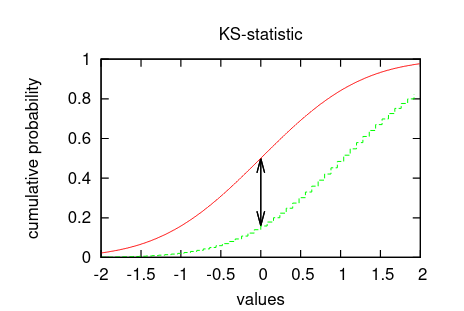
\includegraphics[scale=0.6]{images/ks_statis.png}
\end{figure}

Para o problema de classificação binária o KS pode ser calculado a partir da \textit{Taxa de Verdadeiros Positivos (TVP)} e da \textit{Taxa de Falso Positivos (TFP)}.
\begin{equation}
    KS = \max(TVP - TFP)
\end{equation}
Abaixo temos o algoritmo para o cálculo do KS de \textit{OneSample} \cite{ashwin}.
\begin{algorithm}[H]
\caption{KS: OneSample($Q,n,F$)}\label{algoritmo:ks}
\textbf{Input:} Quantil $Q$, número de dados $n$ e a função de distribuição $F$. \\
\textbf{Output:} $\hat{D}$, o valor estimado de KS. \\
\begin{algorithmic}[1]
\State Seja $X_{i1} \leq X_{i2} \leq ... \leq X_{ik}$ valores em $Q$
\State $\hat{D}$ $\leftarrow$ $0$ 
\If{cada $x\in (X_{i1},...,X_{ik})$} 
\State $j = \max(p | X_{ip}\leq x)$
\State seja $\hat{i_j}$ aproximadamente o índice de $X_{ij}$
\State $\hat{E}_x = | \frac{\hat{i_j}}{n - F(x)}$
\State $\hat{D} = \max(\hat{D},\hat{E}_x)$
\EndIf
\State \Return $\hat{D}$
\end{algorithmic}
\end{algorithm}


\section{Hiperparâmetros e Model Tuning}
Conforme vimos no Capítulo \ref{chapter:introducao} e será abordado nos próximos Capítulos, muitos modelos de aprendizado supervisionado possuem parâmetros que não podem ser diretamente estimados pelo conjunto de treino. Muitos desses parâmetros afetam a qualidade do modelo prever resultados a partir de novos dados de entrada. Esses parâmetros são intrínsecos dos modelos pois representam características deles, como o número de interações, o termo de regularização, o tamanho da árvore e etc. Esses parâmetros precisam ser escolhidos antes do início do processo de aprendizado do algoritmo, e são denominados de hiperparâmetros e o processo de escolha desses parâmetros visando a melhoria da performance do modelo é conhecido como \textit{tuning hyperparameter} \cite{ian,kuhn,tuning:artigo,hyper:op:theory,grid:book,neural:op}.

Para lidar com os hiperparâmetros existem duas abordagens: escolher eles manualmente 
ou utilizar um algoritmo para escolher automaticamente. A escolha manual requer o entendimento profundo da influência dos hiperparâmetros e como os modelos de aprendizagem de máquina alcançam uma boa generalização. Geralmente consiste em retreinar o modelo varias vezes com apenas a alteração dos hiperparâmetros e validando as performance de cada treino. Por outro lado, a seleção automática de hiperparâmetros reduz a necessidade de entender a fundo sua influência, porém requer um maior poder de processamento computacional.

Idealmente, um algoritmo de aprendizagem usaria apenas o conjunto de dados e geraria uma função, não exigindo ajuste manual de hiperparâmetros. A popularidade de vários  algoritmos como regressão logística e SVMs decorre, em parte, de sua capacidade de trazer resultados satisfatórios com apenas um ou dois hiperparâmetros ajustados. As redes neurais podem também funcionar bem com apenas um pequeno número de hiperparâmetros ajustados, mas muitas vezes se beneficiam significativamente do ajuste de quarenta ou mais hiperparâmetros. O ajuste de hiperparâmetros pode funcionar muito bem quando o usuário tem um bom ponto de partida, como aquele determinado por outros que trabalharam no mesmo tipo de aplicativo e arquitetura, ou quando o usuário tem meses ou anos de experiência em explorar valores de hiperparâmetros para redes neurais aplicadas a tarefas semelhantes. No entanto, para muitas aplicações, esses pontos de partida não estão disponíveis. Nesses casos, algoritmos automatizados podem encontrar valores úteis dos hiperparâmetros\cite{tree:tunning}.

Estamos tentando encontrar um valor dos hiperparâmetros que otimize uma função objetivo, como o erro de validação, às vezes sob restrições. Portanto, é possível, em princípio, desenvolver algoritmos de otimização de hiperparâmetros que envolvam um algoritmo de aprendizado de máquina e escolha seus hiperparâmetros, ocultando do usuário do algoritmo de aprendizado o ajuste dos hiperparâmetros. Infelizmente, a otimização de hiperparâmetros dos algoritmos geralmente têm seus próprios hiperparâmetros, como o intervalo de valores que deve ser explorado para cada um dos hiperparâmetros do algoritmo de aprendizado de máquina. No entanto, esses hiperparâmetros secundários são geralmente mais fáceis de escolher, no sentido de que um desempenho aceitável pode ser alcançado em uma ampla gama de tarefas usando os mesmos hiperparâmetros secundários para todas as tarefas.

O processo de tunar os hiperparâmetros geralmente é tratado como uma problema de otimização caixa-preta. De maneira formal, podemos definir o problema como:
Seja:
\begin{gather*}
    \simbolo{\mathcal{H}}{Espaço de Hiperparâmetro} \mathcal{H} = \mathcal{H}_1 \times \mathcal{H}_2 \times ... \times \mathcal{H}_k
\end{gather*}
O espaço dos hiperparâmetros e um algoritmo $a\in \mathcal{A}$ em que $\mathcal{A}$ é um conjunto de algoritmos de aprendizado de máquina. Cada $\mathcal{H}_i$ representa um conjunto de possíveis valores para o hiperparâmetro $i^{th}$ de $a(i\in\{1,...,k\})$. Seja $\mathcal{D}$ um conjunto de dados em que $D\in \mathcal{D}$ é um conjunto de dados de $\mathcal{D}$. A função $f:\mathcal{A}\times \mathcal{D} \times \mathcal{H}\rightarrow \mathbb{R}$ calcula a performance do modelo pelo algoritmo $a\in \mathcal{A}$ no conjunto de dados $D\in \mathcal{D}$ dado a configuração de hiperparâmetros $h=(h_1,h_2,...,h_k)\in\mathcal{H}$.

Dado $a\in \mathcal{A},\mathcal{H}$ e $D\in \mathcal{D}$ o objetivo da tunar os hiperparâmetros é encontrar $h^*=(h_1^*,h_2^*,...,h_k^*)$ tal que :
\begin{equation}
    h^* = {arg\max}_{h\in\mathcal{H}} f(a,D,h)
\end{equation}

Existem diversas técnicas que buscam otimizar os hiperparâmetros, irei exemplificar algumas, para um estudo mais completo consultar \cite{hyper:op:theory,grid:book,neural:op}.
\subsection{Grid Search}
É um dos métodos mais comuns utilizado para explorar o espaço de configuração de hiperparâmetros é o Grid Search. Ele pode ser considerado uma busca exaustiva ou um método de força bruta que avalia todas as combinações de hiperparâmetros dadas à uma 'grade' de configurações. O Grid Search funciona avaliando o produto cartesiano de um conjunto finito de valores especificado pelo usuário, ele não pode explorar as regiões de bom desempenho por si só. Portanto, para identificar os ótimos globais, o seguinte procedimento precisa ser realizado manualmente \cite{grid:article,grid:book,grid:random:2}.

\begin{enumerate}
    \item Comece com um grande espaço de busca e tamanho de passo definidos. 
    \item Restrinja o espaço de pesquisa e o tamanho do passo com base nos resultados anteriores de hiperparâmetros. 
    \item Repita a etapa 2 várias vezes até que um ótimo seja alcançado.
\end{enumerate}

O Grid Search pode ser facilmente implementado e paralelizado. No entanto, a sua principal desvantagem é a sua ineficiência para alta dimensionalidade de espaço de configuração de hiperparâmetros, já que o número de interações aumenta exponencialmente à medida que o número de hiperparâmetros cresce, esse crescimento exponencial é conhecido como a maldição da dimensionalidade. Para Grid Search, assumindo que existem $k$ parâmetros, e cada um deles com $n$ valores distintos, sua complexidade computacional é de $\mathcal{O}(n^k)$. Logo, o Grid Search só se torna um algorítimo eficiente quando o espaço de configurações de hiperparâmetros é pequeno.

\subsection{Random Search}
Para superar certas limitações do Grid Search, o Random Search foi
proposto \cite{randoms,grid:book,grid:random:2}. Ele é bem semelhante ao Grid Search mas ao invés de testar todos os valores no espaço de configuração ele seleciona aleatoriamente um número pré definido de amostrar entre os limites superior e inferior e em seguida treina essas amostras. Ele é capaz de explorar um espaço de busca maior que o Grid Search, ele é facilmente paralelizado pois cada avaliação é independente. Como o número total de avaliações no Random Search é
definido para um valor fixo $n$ antes do início do processo de otimização, a complexidade computacional  é $\mathcal{O(n)}$. Além disso, Random Search pode detectar o ótimo global ou um ótimo local quando fornecido poder computacional o suficiente.

A principal limitação desses dois métodos é que cada avaliação é independente da avaliação anterior, ou seja, eles perdem muito tempo avaliando combinações ruins de hiperparâmetros.


\subsection{Otimização Bayesiana}
Para resolver a limitação do Random Search e Grid Search, temos os algoritmos de otimização Bayesiana, que são algorítimos interativos que determinam o ponto de avaliação futura com base no resultado obtido na interação passada. Para determinar a próxima configuração de hiperparâmetro, o algoritmo usa dois componentes principais: um modelo substituto e uma função de aquisição (ou seleção).
O modelo substituto (processo gaussiano) visa atender a todos os pontos observados na função objetivo. Depois de obter a distribuição posterior de funções que melhor descreve a função que você deseja otimizar a função de aquisição determina o uso de diferentes pontos para equilibrar o trade-off entre \textit{exploration} e \textit{exploitation} \cite{grid:book,opt:bay}.
\textit{Exploration} consiste em amostrar as instâncias nas áreas que não
foram amostrados, enquanto \textit{exploitation} é para amostrar nas atuais regiões promissoras onde o ótimo global é mais provável, com base na distribuição posterior. Os modelos de otimização Bayesiana equilibram ambos os processos para detectar as atuais regiões mais prováveis e evitar a perda de melhores configurações nas áreas inexploradas.
Os procedimentos do algoritmo são:

\begin{enumerate}
    \item Construir um modelo substituto probabilístico da função objetivo. 
    \item Detecte os valores ideais de hiperparâmetros no
modelo substituto.
\item Aplique esses valores de hiperparâmetros à função objetiva para avaliação.
\item Atualize o modelo substituto com novos resultados.
\item Repita as etapas 2 a 4 até que o número máximo de iterações seja
alcançado.
\end{enumerate}

Assim, o algoritmo de otimização Bayesiana funciona atualizando o modelo substituto após cada
avaliação na função objetivo. A otimização Bayesiana é mais eficiente que Grid Search e o Random Search, pois pode detectar a combinação ideal de hiperparâmetros analisando os valores testados anteriormente.


\section{Árvore de Decisão}
A maioria dos algoritmos de boosting utilizam árvores de decisão como aprendizes básicos. 
Uma árvore é uma coleção de elementos chamados de nós, dentre os quais um é distinguido como uma raiz, juntamente com uma relação de “paternidade” que impõe uma estrutura hierárquica sobre os nós.

Uma Árvore de Decisão é:
\begin{itemize}
    \item um nó folha (ou nó resposta) que contém o nome de uma classe ou o símbolo nulo (nulo indica que não é possível atribuir nenhuma classe ao nó por não haver nenhum exemplo que corresponda a esse nó)
\item um nó interno (ou nó de decisão) que contém o nome de um atributo; para cada possível valor do atributo, corresponde um ramo para uma outra árvore de decisão.
\end{itemize}
E temos uma estrutura típica para uma árvore de decisão:
\begin{itemize}
    \item Nós internos são rotulados com atributos.
    \item Folhas são rotuladas com classes
    \item Ramos são rotulados com valores (atributos categóricos) ou com intervalos (atributos numéricos).
\end{itemize}
Uma árvore de decisão é uma representação de uma função que mapeia um vetor de valores de atributos para um único valor de saída, uma "decisão". Uma árvore de decisão chega à sua decisão realizando uma sequencia de testes, começando na raiz e seguindo o ramo apropriado até que uma folha seja alcançada. Cada nó interno na árvore corresponde a um teste do valor de uma das entradas atributos, os ramos do nó são rotulados com os possíveis valores do atributo, e os nós folha especificam qual valor deve ser retornado pela função. O processo de aprendizado de uma árvore de decisão é chamado de indução da árvore de decisão. A ideia do algoritmo é escolher as divisões internas da árvore que melhor explicam os dados e é, em si, uma pequena árvore. Na figura \ref{fig:ex:arvore} temos um exemplo de uma aŕvore de decisão treinada \cite{russel}.

\begin{figure}[H]
 \caption{Exemplo de uma árvore de decisão \cite{russel}.}
 \label{fig:ex:arvore}
 \centering
 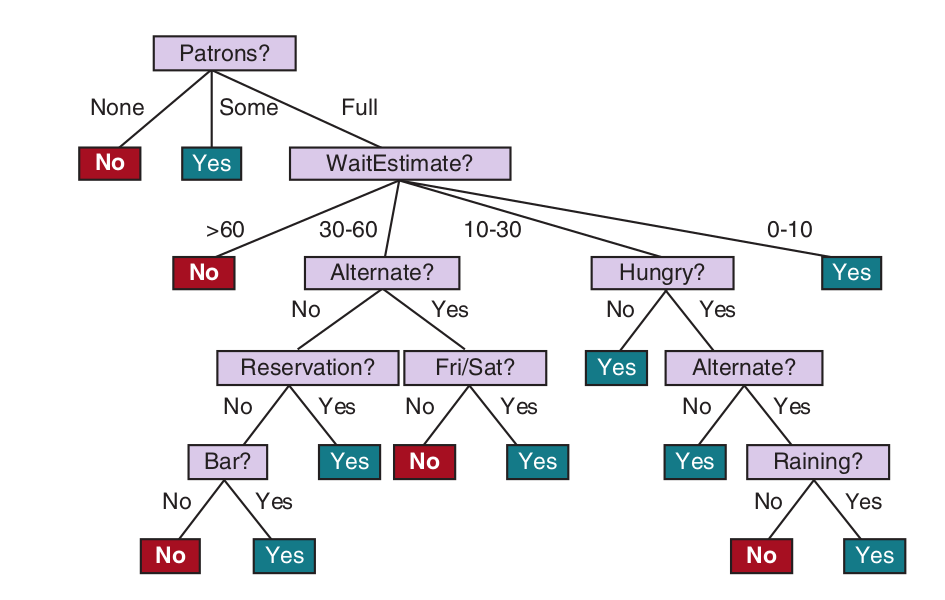
\includegraphics[scale=0.4]{images/exemplo_arvore.png}
\end{figure}

O processo de aprendizado das árvores de classificação consiste em várias iterações para escolher as melhores divisões a partir dos dados de treinamento fornecidos, de acordo com critérios. Os critérios mais comuns de otimização são
geralmente advindos da Teoria da Informação, como o Índice de Gini e a Entropia Cruzada.
O índice de Gini, $G(D)$ no nó $S$ na árvore de decisão pode ser definido como:
\begin{gather*}
    G(S) = 1 - \sum_{i=1}^cp_i^2
\end{gather*}
O algoritmo \ref{algoritmo:arvore} mostra o pseudo código para o algoritmo de árvore de decisão \cite{tree:algor:risk}.
\begin{algorithm}[H]
\caption{Árvore de decisão.\label{algoritmo:arvore}}
\textbf{Input:} Conjunto de treino $D=\mathbf{x}^{(1)},y^{(1)}),(\mathbf{x}^{(2)},y^{(2)}),(\mathbf{x}^{(i)},y^{(j)}$. Atributos $A=(a_1,a_2,..._a_k)$. Método de seleção do atributo: Utilizaremos o \textit{Gain Ratio} para separar o atributo e o sub conjunto de dados $GR(D,a)=\frac{G(D,a)}{Entropia(a)}$, em que $Entropia(D)= \sum_{i=1}^c-p_ilog_2p_i$ e o $G(D,a)=Entropia(D) - \sum_{v\in Values(a)}^{} \frac{|D_v|}{D}Entropia(D_v)$, em que $Values(a)$ são todos os possíveis valores do atributo $a$ e $D_v$ é um sub conjunto do nosso conjunto de dados $D$ que para cada atributo tem o valor $v$.\\
\textbf{Output:} Árvore de decisão. \\
\begin{algorithmic}[1]
\State criar o nó $N$
\If{as amostras de $D$ estão na mesma classe $C$} 
\State \Return $N$ como nó folha rotulado com a classe $C$
\EndIf
\If{$A \neq 0 $ ou o valor do atributo em $D$ são o mesmo}
\State \Return $N$ como nó folha rotulado com a classe em $D$
\EndIf
\State ache o melhor atributo $a\in A$ utilizando um método de seleção de atributo
\State \For{cada valor $a^y$ de $a_*$}
\If{$D_v \neq 0$}
\State colocar a folha com a maioria das classes em $D$ para o nó $N$
\Else
\State colocar o nó retornado pelo $TreeGenerate(D_V,A)$ para o nó $N$
\EndIf
\EndFor
\end{algorithmic}
\end{algorithm}


Hiperparâmetros típicos de árvores de classificação referem-se à estrutura real da árvore. Como por exemplo o hiperparâmetro de profundidade máxima controla a profundidade que a árvore pode crescer, ou seja, quantas divisões serão
tomadas, amostras mínimas de folhas controla o número mínimo de amostras que cada folha precisa ter. A tabela \ref{tabela:ex:hiper} abaixo mostra alguns exemplos de hiperparâmetros de modelos de árvore de decisão \cite{tree:tunning} \cite{ian}.
\begin{table}[htb]
\centering
\caption{Exemplo de hiperparâmetros em árvore de decisão\cite{tuning:artigo}\cite{ian}.}
\label{tabela:ex:hiper}
\begin{tabular}{|p{4cm}|p{8cm}|p{3cm}|} 
 \hline
\textbf{Hiperparâmetro} & \textbf{Descrição} & \textbf{Tipo da variável} \\
  \hline
  \textit{min\_samples\_split} & O número mínimo de amostras necessárias para dividir um nó interno. & int ou float \\
  \hline
  \textit{max\_depth} & A profundidade máxima da árvore. Se Nenhum, os nós serão expandidos até que todas as folhas sejam puras ou até que todas as folhas contenham menos que min\_samples\_split amostras. & int \\
  \hline
  \textit{splitter} & A estratégia usada para escolher a divisão em cada nó. As estratégias suportadas são “melhores” para escolher a melhor divisão e “aleatórias” para escolher aleatoriamente. & string \\
  \hline
  \textit{min\_weight\_fraction\_leaf} & A estratégia usada para escolher a divisão em cada nó. As estratégias suportadas são “melhores” para escolher a melhor divisão e “aleatórias” para escolher aleatoriamente. & string \\
  \hline
  \textit{min\_samples\_leaf} & A fração ponderada mínima da soma total dos pesos (de todas as amostras de entrada) necessária para estar em um nó folha. & float \\
  \hline
  \textit{max\_features} & O número de features a serem considerados ao procurar a melhor divisão. & int ou float \\
  \hline
  \textit{random\_state} & Gerador de números aleatórios. & int \\
  \hline
  \textit{min\_impurity\_decrease} & Um nó será dividido se esta divisão induzir uma diminuição da impureza maior ou igual a este valor.. & float \\
  \hline
  \textit{class\_weight} & Pesos associados a classes no formato (class\_label: weight). Se não for fornecido, todas as classes devem ter peso um. Para problemas de múltiplas saídas, uma lista de dicionários pode ser fornecida na mesma ordem das colunas de $y$. & dicionário, lista de dicionário, “balanced” ou None\\
  \hline
\end{tabular}
\end{table}


\chapter{Algoritmos de Gradient Boosting}
\label{chapter:algoritmos-boosting}
\textit{Gradient Boosting Machines} (GBM) é um algoritmo de aprendizado de máquina, baseado na ideia de modelos aditivos de estatística e descida de gradiente. O GBM funciona construindo um modelo aditivo avançado \textit{stagewise} realizando gradiente descendente no espaço de função, conforme proposto por \cite{greedy}. O \textit{Gradient Boosting} é um algoritmo de aprendizado de máquina amplamente utilizado devido à sua eficiência, precisão e interpretabilidade.
\section{Additive Model}
Um modelo aditivo é uma técnica de regressão onde a ideia básica é aproximar um conjunto de dados usando uma soma de funções suaves do indivíduo características dos dados observados, em vez de uma superfície de regressão geral complexa \cite{persu:regre}.

Considere o conjunto de dados $\{(\mathbf{x}^{(1)},y^{(1)}),(\mathbf{x}^{(2)},y^{(2)}),...,(\mathbf{x}^{(i)},y^{(i)})\}$, em que $\mathbf{x}$ são os preditores e $y$ a saída, o modelo aditivo pode ser escrito da seguinte forma

\begin{equation}
    E|y^{(i)}|x^{(1)},x^{(2)},...,x^{(i)}| = \beta_0 + \sum_{j=1}^pf_j(x^{(ij)})
\end{equation}
Ou
\begin{equation}
    Y = \beta_0 + \sum_{j=1}^pf_j(\mathbf{X}^{(:,j)}) + \epsilon
\end{equation}
As funções $f_j(x^{(ij)}$ são conhecidas como funções de suavização, ou seja, ao invés de utilizar uma regra complexa de regressão, usamos a soma de funções de suavização.

\section{\textit{Gradient Descent}}
Podemos separar os métodos de solução de problemas de otimização entre determinísticos e métodos estocásticos. Abordagens determinísticas são geralmente mais simples que as estocásticas, porém, o risco de ficar preso em um mínimo local é significativamente maior. O gradiente descendente é um método estocásticos.

\begin{figure}[h]
 \caption{Exemplo de otimização pelo gradiente descendente.}
 \label{fig:ex:grad}
 \centering
 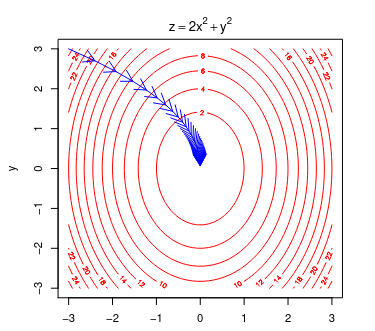
\includegraphics[scale=0.4]{images/ilustra_grad.png}
\end{figure}

A versão básica do algoritmo tem como objetivo minimizar uma função objetiva $F(\theta)$. Esse algorítimo tem uma taxa de aprendizado\simbolo{\eta,LR}{\textit{learning rate}, taxa de aprendizado}$\eta$ para controlar o quanto os coeficientes de $\theta$ podem mudar em cada interação \cite{russel,hastie,ian,over:gradia,mit:parallel,convex:opt}. 

Podemos escrever o gradiente descendente como:
\begin{equation} \label{eq:gradiente}
    \theta_t = \theta_{t-1} - \eta \cdot \nabla{\theta_{t-1}}F(\theta_{t-1};\mathbf{x}^{(i)},y^{(i)})
\end{equation}

Uma execução de descida de gradiente executará a atualização acima $t = M$ vezes e pode ser interpretada como $M$,a atualização, gerando vetores $v_m$ da forma $v_m = - \eta \cdot \nabla{\theta_{t-1}}F(\theta_{t-1};\mathbf{x}^{(i)},y^{(i)})$. Denotando $v_0 = \theta_0$, os valores iniciais dos parâmetros antes da otimização, os parâmetros finais podem ser escritos como:
\begin{equation}
    \theta^* = \sum_{m=0}^{M-1}v_m
\end{equation}



\section{\textit{Boosting}}
\textit{Boosting} é uma das ideias de aprendizado mais poderosas introduzidas nas últimas décadas. Ele foi originalmente projetado para problemas de classificação mas pode ser utilizado para problemas de regressão.  A ideia por tras do \textit{boosting} é combinar a saídas de muitos classificadores “fracos” para produzir um “comitê” poderoso, ou seja, criar um aprendiz "poderoso" a partir de uma combinação de aprendizes "fracos" \cite{brief:intro:boost,hastie}.

Um classificador fraco é aquele cuja taxa de erro é apenas ligeiramente melhor do que uma adivinhação aleatória. O objetivo do \textit{boosting} é aplicar sequencialmente o
algoritmo de classificação "fraco" para várias versões, produzindo assim uma sequência de classificadores fracos $G_m(x),m= 1, 2, 3, ..., M$.
As previsões de todos eles são combinadas por meio de uma ponderação para produzir a previsão final:
\begin{equation}
    G(x) = sign(\sum_{m=1}^M\alpha_mG_m(x))
\end{equation}

Em que $\alpha_1,\alpha_2, \alpha_M$ são calculados pelo algoritmo de boosting e cada contribuição segue um peso em $G_m(x)$. Esse algoritmo mostrado pela equação acima é conhecido como AdaBoost \cite{adaboost}. Abaixo temos um esquemático de como os classificadores são treinados na versão com peso do conjunto de dados e depois combinado com a predição final.
\begin{figure}[h]
 \caption{Esquemático do algoritmo AdaBoost \cite{hastie}.}
 \label{fig:ex:adaboost}
 \centering
 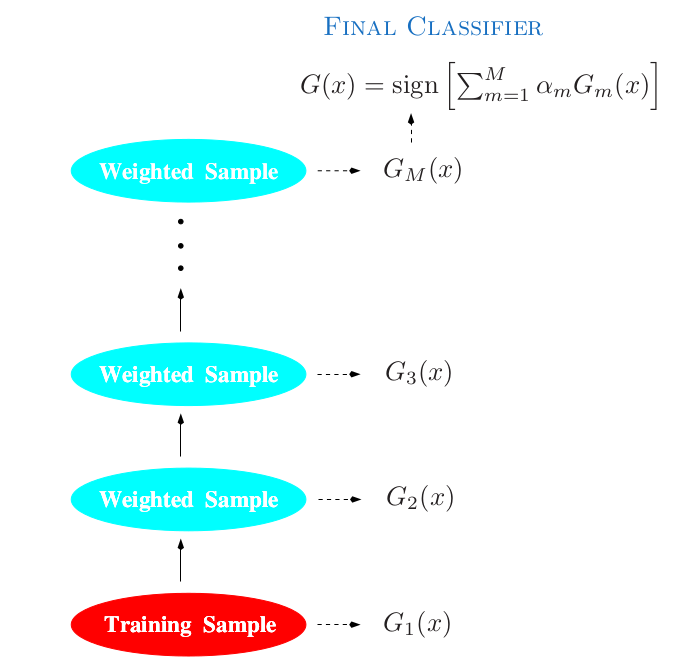
\includegraphics[scale=0.3]{images/adaboost.png}
\end{figure}

O algoritmo \ref{algoritmo:adaboost} mostra o detalhe do algoritmo de AdaBoost \cite{adaboost,hastie}.
\begin{algorithm}[H]
\caption{AdaBoost M1}\label{algoritmo:adaboost}
\begin{algorithmic}[1]
\State Iniciar as observações com pesos $w_i = 1/N, i=1,2,3,...,N$
\State \For{$m=1$ até $M$:}
\State Fit o classificador $G_m(x)$ no conjunto de treino utilizando os pesos $w_i$
\State calcule o erro $err_m = \frac{\sum_{i=1}^Nw_i\mathbf{1}(y_i\neq G_m(x_i))}{\sum_{i=1}^Nw_i}$
\State Calcule $\alpha_m = log((1-err_m)/err_m)$
\State $w_i \rightarrow w_i\cdot exp[\alpha_m \cdot \mathbf{1}(y_i\neq G_m(x_i))],i=1,2,...,N$
\EndFor
\State \Return $G(x) = sign(\sum_{m=1}^M\alpha_mG_m(x))$
\end{algorithmic}
\end{algorithm}

\section{GBMs}
\textit{Gradient Boosting Machine} utiliza o conceito de modelo aditivo e é uma combinação do gradiente descente com o \textit{boosting} \cite{greedy}. O algoritmo GBM funciona otimizando qualquer função de perda diferenciável, usando Gradiente descendente. No entanto, a otimização não é feita em termos de otimização numérica (ou seja, atualizando um vetor de parâmetros $\theta$), mas por funções de "bossting" na direção do gradiente da função de perda. Como os GBMs lidam com dados finitos, eles otimizam as funções em termos do conjunto de dados supervisionado, nosso conjunto $(\mathbf{x}^{(i)} , y^{(i)})$, o modelo final de GBM será:

\begin{equation}
    F_M(x) = F_0(x) + \sum_{m=1}^MF_m(x)
\end{equation}

As funções $F_m(x)$ são funções construídas de forma \textit{stagewise}, assim como o $\theta_t$ em gradiente descendente. As funções base são aprendizes, e podem ser parametrizadas como $\beta_m h(\mathbf{x};a_m)$, onde $\beta_m$
é um peso, e $\alpha_m$ os parâmetros do aprendiz $h$. Na maioria das implementações, as funções básicas são aprendizes baseados em árvore, mas podem ser qualquer aprendiz em que seja seja possível atribuir pesos. Também, dada uma função de perda $L(y_i , F_m(x_i))$, gostaríamos de encontrar todos os valores ótimos de $\beta_m$ e $\alpha_m$ que minimizam a função perda, ou seja:
\begin{equation*}
    \{\beta_m,\alpha_m\}_1^M = {\arg\min}_{\{\beta'_m,\alpha'_m\}_1^M}\sum_{i=1}^n L\Biggl(y^{(i)},\sum_{m=1}^M\beta'_mh(\mathbf{x}^{(i)};\alpha'_m)\Biggl)
\end{equation*}
No entanto, na maioria das situações, a otimização acima é inviável, portanto, a abordagem \textit{"greedy-stagewise”} é otimizar cada par $\beta_m$ e $\alpha_m$ em um modelo \textit{stagewise}, ou seja, para cada $m = 1, 2, ..., M$.
\begin{equation}\label{eq:interacoes}
    (\beta_m,\alpha_m) = {\arg\min}_{\beta,\alpha}\sum_{i=1}^n L\Biggl(y^{(i)},F_{m-1}\mathbf{x}^{(i)} + \beta h(\mathbf{x}^{(i)};\alpha)\Biggl)
\end{equation}
Utilizando a notação vetorizada 
\begin{equation}
    F_m(\mathbf{X}) = F_{m-1}(\mathbf{X}) + \eta \Delta_m(X)
\end{equation}
$\beta_m h(\mathbf{x}^{(i)};\alpha_m)$ pode ser interpretado como o melhor passo "greedy" em direção à estimativa, $F^*(x)$, esta pode ser vista como uma atualização do método do gradiente descendente. O análogo de $\nabla{\theta_{t-1}}$ no gradiente descente numérico é o gradiente da função de perda $L$ com relação à última estimativa $F_{m−1}(x)$ \cite{greedy}.

\begin{equation}
    -g_m(\mathbf{x}^{(i)}) = -\Bigg[\frac{\partial L(y^{(i)},c^{(i)})}{\partialF(\mathbf{x}^{(i)})}\Bigg]
\end{equation}
Em que $F(x)=F_{m-1}(x)$.

Na literatura, esse gradiente da função de perda $L$ em relação à última previsão $\hat{y}_{m−1}$. Essa última previsão às vezes é chamada de pseudo-residual e definida como $\mathbf{r}_{m-1}$. 
\begin{equation}
    \mathbf{r}_{m_1} = \nabla F_{m-1}(\mathbf{X})L(y,F_{m-1}(\mathbf{X})) = \nabla \hat{y}_{m-1}L(y,\hat{y}_{\mathbf{m-1}})
\end{equation}

O algoritmo GBM ajusta um aprendiz $h(x;\alpha_m)$ com peso $\beta$ usando os pseudo-resíduos, não o $\mathbf{X}$ original. A versão final do algoritmo é definida como:

\cite{hastie,greedy}.
\begin{algorithm}[H]
\caption{Gradient Boost($\mathbf{X},y,M,\eta$)}\label{algoritmo:gradboost}
\begin{algorithmic}[1]
\State $F_0(\mathbf{X} = \arg\min_v\sum_{i=1}^n L(y^{(i)},v)$
\State \For{$m=1$ até $M$:}
\State $\mathbf{r}_{m_1} = \nabla \hat{y}_{m-1}L(y,\hat{y}_{\mathbf{m-1}})$ \Comment{Treinar o aprendiz base para minimizar o erro quadrático}
\State $\alpha = {\arg\min}_{\alpha,\beta}\sum_{i=1}^n(\mathbf{r}_{m-1}^{(i)}-\beta h(\mathbf{x}^{(i)};\alpha))^2$
\State $\beta = {\arg\min}_{\beta}\sum_{i=1}^nL(y^{(i)},F_{m-1}(\mathbf{x}^{(i))}+\beta h(\mathbf{x}^{(i))};\alpha_m)$
\State $\Delta_m(X) = \beta_mh(\mathbf{X};\alpha_m)$
\State $F_m(\mathbf{X}) = F_{m-1}(\mathbf{X}) + \eta \Delta_m(X)$
\EndFor
\State \Return $F_m$
\end{algorithmic}
\end{algorithm}

\section{XGBoost, CatBoost e LightGBM}
Os três algoritmos no escopo do trabalho: XGBoost (\textit{Xtreme Gradient Boosting}), CatBoost (\textit{Category Boosting}) e LightGBM (\textit{Light Gradient Boosting Machine}) são todos variantes de algoritmos de \textit{Gradient Boosting}. Todos podem ser utilizados como Regressor (prevendo variáveis contínuas) ou um Classificador (prevendo variáveis categóricas).

XGBoost é uma solução altamente escalável, flexível e versátil, foi projetado para explorar recursos corretamente e superar as limitações do aumento de gradiente anterior. A principal diferença entre XGBoost e outros algoritmos de gradiente é que ele usa uma nova técnica de regularização para controlar o overfitting. Portanto,
é mais rápido e mais robusto durante o ajuste do modelo. A técnica de regularização é feita adicionando um novo termo a função de perda, como:

\begin{equation}
    L(\phi) = \sum_{i=1}^nL(\hat{y}_i,y_i) + \sum_{m=1}^M\Omega(f_k)
\end{equation}

Em que :
\begin{equation}
    \Omega(f) = \gamma T + \frac{1}{2}\lambda||w||^2
\end{equation}


XGBoost usa um novo ganho
\begin{equation} \label{eq:gain}
    Gain = \frac{1}{2}\Bigg[ \frac{(\sum_{i\in I_L}g_i)^2}{\sum_{i\in I_L}h_i + \lambda} + \frac{(\sum_{i\in R_L}g_i)^2}{\sum_{i\in R_L}h_i + \lambda} - \frac{(\sum_{i\in I}g_i)^2}{\sum_{i\in I}h_i + \lambda} \Bigg] - \gamma
\end{equation}

Em que
\begin{equation}
    g_i = \partial_{\hat{y}_i}L(\hat{y}_i,y_i) \\ 
    h_i = \partial^2_{\hat{y}_i}L(\hat{y}_i,y_i)
\end{equation}
Assuma que $I_L$ e $I_R$ são os conjuntos de instâncias da esquerda e nós direitos após a divisão e $I = I_L\cup I_R$ \cite{article:xgboost,doc:xgboost}.

\begin{figure}[H]
 \caption{Exemplo do cálculo da estrutura do cálculo do score para uma árvore \cite{article:xgboost}.}
 \label{fig:ex:xgboost}
 \centering
 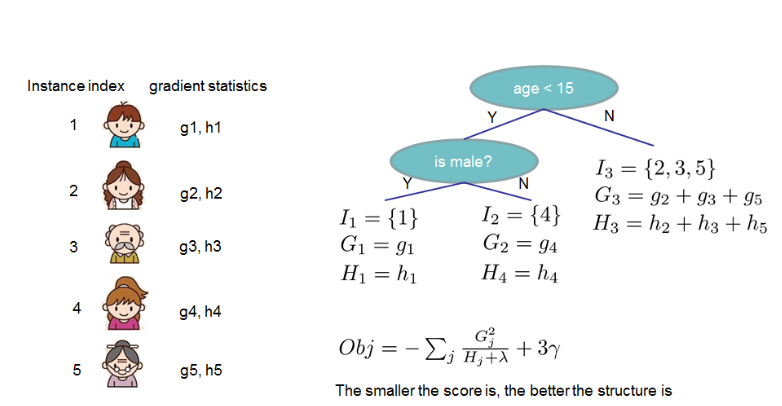
\includegraphics[scale=0.4]{images/estrutura_score_xgboost.png}
\end{figure}

CatBoost (para “impulsionamento categórico”) concentra-se em colunas categóricas usando técnicas de permutação, one\_hot\_max\_size (OHMS) e estatísticas baseadas em alvo. CatBoost resolve o crescimento exponencial da combinação de recursos usando o método greedy em cada nova divisão da árvore atual. Além disso a construção é feita por arvores simétricas e o algoritmo suporta colunas categóricas \cite{article:catboost,doc:catboost}.

O LightGBM é parecido com o XGBoost com algumas alterações: uma nova técnica para estimar o ganho de informação chamada \textit{gradient-based one-side sampling} (GOSS). Uma vez que uma das tarefas mais demoradas no processo de aprendizagem no aumento de gradiente é encontrar a divisão para as árvores, geralmente algum tipo de amostragem é feito nesta etapa para fins de eficiência \cite{article:lgbm,doc:LGBM}.

Temos abaixo um comparativo com maiores detalhes de cada algoritmo.
\subsection{Divisões de nó}
Antes de começar o aprendizado os algortimos precisam criar pares de divisões de recursos, por exemplo (idade,$<15$), (idade,$>20$), (quantidade, >1000). Esses pares de divisão de recurso são construídos com base em histograma e são usados durante o processo de aprendizado como possíveis divisões de nó. Esse método de pré-processamento é mais rápido do que o algoritmo \textit{greedy}, que enumera linearmente todas as divisões possíveis para recursos contínuos.

O \textbf{XGboost} não utiliza nenhuma técnica de amostragem ponderada, ele utiliza algoritmos puramente baseados em histogramas o que torna seu processo de divisão mais lento em comparação com GOSS e MVS.

O \textbf{Catboost} oferece uma nova técnica chamada \textit{Minimal Variance Sampling} (MVS), que é uma versão de amostragem ponderada do \textit{Stochastic Gradient Boosting}. Nesta técnica, a amostragem ponderada ocorre no nível da árvore e não no nível da divisão. As observações para cada árvore de reforço são amostradas de forma a maximizar a precisão da pontuação dividida.

O \textbf{LightGBM} oferece amostragem unilateral baseada em gradiente (GOSS) que seleciona a divisão usando todas as instâncias com grandes gradientes (ou seja, grande erro) e uma amostra aleatória de instâncias com pequenos gradientes. Para manter a mesma distribuição de dados ao calcular o ganho de informação, o GOSS introduz um multiplicador constante para as instâncias de dados com pequenos gradientes. Assim, o GOSS consegue um bom equilíbrio entre aumentar a velocidade, reduzindo o número de instâncias de dados, e manter a precisão das árvores de decisão aprendidas.

\subsection{Crescimento da Árvore}
O \textbf{XGboost} divide as árvores até o hiperparâmetro max\_depth especificado e logo em seguida começa a podar a árvore para trás e remove as divisões além das quais não há ganho positivo. Ele usa essa abordagem, pois às vezes uma divisão sem redução de perda pode ser seguida por uma divisão com redução de perda. O XGBoost também pode executar o crescimento da árvore folha a folha (como LightGBM).

\textbf{Catboost} cresce uma árvore equilibrada. Em cada nível dessa árvore, o par de divisão de recursos que traz a menor perda (de acordo com uma função de penalidade) é selecionado e é usado para todos os nós do nível. É possível alterar sua política usando o parâmetro grow\_policy.

O \textbf{LightGBM} usa crescimento de árvore folha a folha (melhor primeiro). Opta por cultivar a folha que minimiza a perda, permitindo um crescimento de uma árvore desequilibrada. Como não cresce em nível, mas em folha, o \textit{overfitting} pode acontecer quando os dados são pequenos. Nesses casos, é importante controlar a profundidade da árvore.

A figura \ref{fig:three graphs} mostra o comparativo do crescimento de árvore de cada algoritmo.

\begin{figure}[H]
     \centering
     \begin{subfigure}[b]{0.4\textwidth}
         \centering
         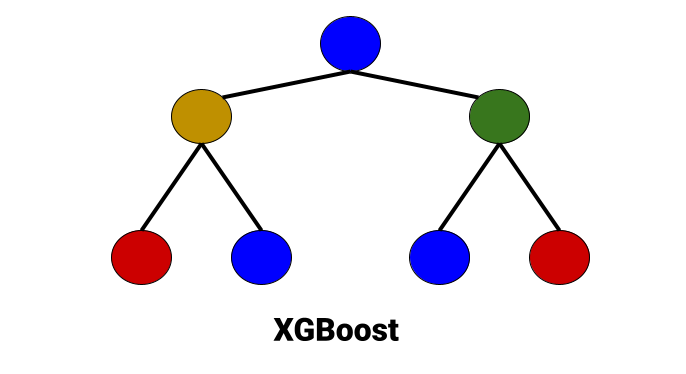
\includegraphics[width=\textwidth]{images/XGboost.png}
     \end{subfigure}
     \hfill
     \begin{subfigure}[b]{0.4\textwidth}
         \centering
         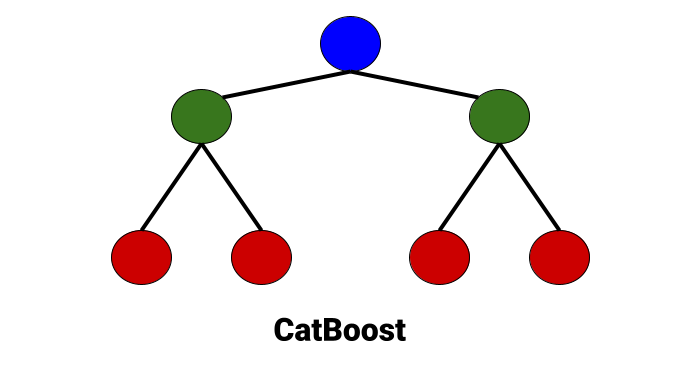
\includegraphics[width=\textwidth]{images/CatBoost.png}
     \end{subfigure}
     \hfill
     \begin{subfigure}[b]{0.4\textwidth}
         \centering
         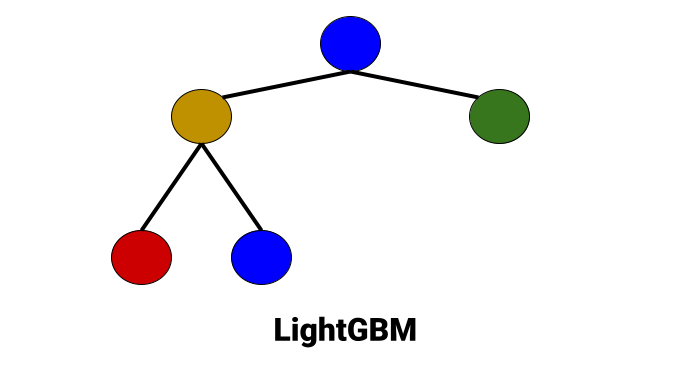
\includegraphics[width=\textwidth]{images/LGBM.png}
     \end{subfigure}
        \caption{Comparativo do crescimento da Árvore no XGBoost, CatBoost e LightGBM}
        \label{fig:three graphs}
\end{figure}


\subsection{Valores \textit{Missing}}
No \textbf{XGboost} e \textbf{LightGBM}, os valores \textit{missing} serão alocados para o lado que reduz a perda em cada divisão. Enquanto o \textbf{Catboost} tem dois modos para processar valores ausentes, “Min” e “Max”. Em “Min”, os valores ausentes são processados como o valor mínimo para um recurso (eles recebem um valor menor que todos os valores existentes). Dessa forma, é garantido que uma divisão que separa os valores ausentes de todos os outros valores seja considerada ao selecionar as divisões. “Max” funciona exatamente da mesma forma que “Min”, apenas com valores máximos.

\subsection{\textit{Feature Importance}}
O \textbf{XGboost} e o \textbf{LightGBM} têm dois métodos semelhantes: O primeiro é “Ganho”, que foi explicado na equação \ref{eq:gain}. É a melhoria na precisão (ou ganho total) trazida por um recurso para os ramos em que está. O segundo método tem um nome diferente em cada pacote: \textit{split} (LightGBM) e \textit{Frequency/Weight} (XGBoost). Este método calcula o número relativo de vezes que um determinado recurso ocorre em todas as divisões das árvores do modelo. Esse método pode ser influenciado por recursos categóricos com um grande número de categorias.

O \textbf{XGboost} possui mais um método, \textit{Coverage}, que é o número relativo de observações relacionadas a uma feição. Para cada recurso, contamos o número de observações usadas para decidir o nó folha.

\textbf{Catboost} tem dois métodos: O primeiro é \textit{PredictionValuesChange}. Para cada recurso, \textit{PredictionValuesChange} mostra quanto, em média, a previsão muda se o valor do recurso mudar. Uma característica teria uma importância maior quando uma mudança no valor da característica causa uma grande mudança no valor previsto. Este é o método de cálculo de importância de recurso padrão para métricas não classificadas. O segundo método é \textit{LossFunctionChange}. Esse tipo de importância de recurso pode ser usado para qualquer modelo, mas é particularmente útil para modelos de classificação. Para cada característica o valor representa a diferença entre o valor de perda do modelo com esta característica e sem ela. Como é computacionalmente caro retreinar o modelo sem um dos recursos, esse modelo é construído aproximadamente usando o modelo original com esse recurso removido de todas as árvores do conjunto. O cálculo dessa importância de recurso requer um conjunto de dados.

\subsection{Variáveis Categóricas}
O \textbf{XGboost} não possui um método embutido para recursos categóricos. A codificação (\textit{one-hot-encoding}, codificação de destino, etc.) deve ser realizada pelo usuário.

\textbf{Catboost} usa uma combinação de codificação one-hot e uma codificação média avançada. Para recursos com baixo número de categorias, ele usa \textit{one-hot-encoding}. O número máximo de categorias para \textit{one-hot-encoding} pode ser controlado pelo parâmetro one\_hot\_max\_size. Para as colunas categóricas restantes, CatBoost usa um método eficiente de codificação, que é semelhante à codificação média, mas com um mecanismo adicional destinado a reduzir o \textit{overfitting}.

\textbf{LightGBM} divide recursos categóricos particionando suas categorias em 2 subconjuntos. A ideia básica é classificar as categorias de acordo com o objetivo do treinamento em cada divisão, o valor final que vai ser treinado no modelo tem que ser um valor númerico.

A Tabela \ref{tabela:ex:dif:algo} resume essas principais diferenças entre os algoritmos.
\begin{table}[H]
\centering
\caption{Principais características do XGBoost, CatBoost e LightGBM}
\label{tabela:ex:dif:algo}
\begin{tabular}{|p{4cm}|p{3cm}|p{3cm}|p{3cm}|} 
 \hline
& \textbf{XGBoost} & \textbf{CatBoost} & \textbf{LightGBM} \\
  \hline
  \textbf{Desenvolvedor} & DMLC & Yandex & Microsft \\
  \hline
  \textbf{Ano de Release} & 2014 & 2017 & 2016 \\
  \hline
  \textbf{Simetria da Árvore} & Assimétrica Level-wise  & Simétrica & Assimétrica Leaf-wise \\
  \hline
  \textbf{Método de Splitting} & Algoritmos de histogramas & Greedy & GOSS \\
  \hline
  \textbf{Colunas Numéricas} & Suporta & Suporta & Suporta \\
  \hline
  \textbf{Colunas Categóricas} & Não Suporta (conveter utilizando one-hot-encoding) & Suporta & Não Suporta (converter para numérico ou ordinal) \\
  \hline
  \textbf{Colunas de Texto} & Não Suporta & Suporta & Não Suporta \\
  \hline
  \textbf{Valores missing} & Interpreta como NaN ou zero & Interpreta como NaN ou zero & Interpreta como NaN ou zero \\
  \hline
\end{tabular}
\end{table}

\section{Hiperparâmetros} \label{cap3:hiper}
Conforme vimos na seção anterior, uma das principais diferença entre o XGBoost e CatBoost para o LGBM é que o LGBM cultiva folhas de árvores, enquanto que os outros algoritmos utilizam uma abordagem de profundidade. Isso impacta em como cada valor de hiperparâmetro deve ser escolhido e quais valores devem ser otimizados e estudados. Cada algoritmo pode ter mais de 20 hiperparâmetros. Abaixo temos os hiperparâmetros mais comuns e alguns deles serão analisados na primeira parte desse estudo. Na segunda parte, ao utilizar o Optuna para tunar o modelo podemos inserir mais hiperparâmetros.
\begin{itemize}
    \item \textbf{learning\_rate:} Taxa de aprendizado $\eta$, é o parâmetro que discutimos em \ref{eq:gradiente}, ele é responsável por controlar a influencia de cada novo aprendiz, ou seja, ele basicamente determina o tamanho do passo de cada interação enquanto se move em direção a um mínimo da função de perda.
    \item \textbf{num\_leaves:}Este hiperparâmetro controla o número máximo de folhas a crescer em cada iteração, e é a principal forma de controlar a complexidade do modelo.
    \item \textbf{max\_depth:} Profundidade máxima de uma árvore. Aumentar esse valor tornará o modelo mais complexo e com maior probabilidade de \textit{overfit}.
    \item \textbf{n\_estimators:} O número de estimadores ou iterações de aumento no processo de aumento de gradiente. Isto é o parâmetro $M$ na Equação \ref{eq:interacoes} e controla quantas árvores são cultivadas no treinamento do modelo. Normalmente, quanto maior o número de iterações, melhor o modelo ficará, até que comece \textit{overfitting} nos dados de treinamento.
    \item \textbf{early\_stopping\_rounds:} É um parâmetro utilizado para reduzir o \textit{overfitting} ele recebe um valor inteiro que informa ao algoritmo quando parar se não houver mais melhorias na métrica de avaliação. Pode evitar o \textit{overfitting} e melhorar o desempenho do seu modelo. Não necessariamente é um parâmetro que queremos 'tunar', mas vamos utilizar ele para reduzir o \textit{overfitting}.
    \item \textbf{reg\_lambda:} Termo de regularização $L2$ nos pesos.
\end{itemize}

\section{Optuna}
Uma das tarefas mais importantes na construção de modelos de aprendizado de máquina é a otimização de hiperparâmetros. Uma otimização correta dos hiperparâmetros se reflete diretamente no desempenho do modelo e nos últimos anos essa frente de otimização dos hiperparâmetros tem tido grande avanço na pesquisa e diversas soluções existem atualmente. Podemos citar Spearmint, Vizer, AutoSklearn, HyperOpt, dentre outras. Entretanto cada ferramente propõe uma própria abordagem de usabilidade podendo se tornar mais ou menos flexível dependo do caso ou complexidade do modelo. Ou seja, a escalabilidade dessas aplicações pode ser dificultada. Com isso, surgiu o Optuna um framework Open Source para otimização de hiperparâmetros, cujo objetivo é unificar os paradigmas de otimização sob uma filosofia apoiada em três pilares: \textit{API design-by-run}, implementação eficiente, facilidade de configuração e versatilidade de arquitetura \cite{optuna}\cite{doc:optuna}.

Na Tabela \ref{tabela:ex:dif:optuna} temos uma comparação de outros algoritmos de otimização de hiperparâmetros e o Optuna \cite{optuna}.
\begin{table}[h]
\centering
\caption{Comparativo de outros algorítimos de otimização de hiperparâmetros \cite{optuna}.}
\label{tabela:ex:dif:optuna}
\begin{tabular}{|c|c|c|c|c|c|c|} 
 \hline
\textbf{Framework} & \textbf{API} & \textbf{Pruning} & \textbf{Lightweight} & \textbf{Distributed} & \textbf{Dashboard} & \textbf{OSS}\\
  \hline
  SMAC & define and run     & \xmark & \cmark & \xmark & \xmark &\cmark\\
  \hline
  GPyOpt & define and run   & \xmark & \cmark & \xmark & \xmark &\cmark\\
  \hline
  Spearmint & define and run & \xmark & \cmark & \cmark & \xmark &\cmark\\
  \hline
  Hyperopt & define and run & \xmark & \cmark & \cmark & \xmark &\cmark\\
  \hline
  Autotune & define and run & \cmark & \xmark & \cmark & \cmark &\xmark\\
  \hline
  Vizier & define and run & \cmark & \xmark & \cmark & \cmark &\xmark\\
  \hline
  Katib & define and run & \cmark & \xmark & \cmark & \cmark &\cmark\\
  \hline
  Tune & define and run & \cmark & \xmark & \cmark & \cmark &\cmark\\
  \hline
  Optuna & define by run & \cmark & \cmark & \cmark & \cmark &\cmark\\
  \hline
\end{tabular}
\end{table}

Por padrão o Optuna utiliza Tree-Structured Parzen Estimator, um algorítimo de otimização Bayesiana, conforme foi abordado no capitulo \ref{chapter:fundamentos-aprendizado}, mas podem ser utilizados outros algoritmos de otimização. Para mais informações sobre esse tipo de otimização e os outros algoritmos consulte \cite{doc:optuna,hyper:op:theory,grid:book,neural:op,op:TPE}.

Antes de começar a implementar a otimização com Optuna, é necessário definir uma função objetivo. A função objetivo conterá toda a lógica de um processo regular de definição, treinamento e teste de modelo. Após a avaliação do modelo, ele deve retornar a métrica de avaliação que também é escolhida pelo usuário.
A classe Trial será usada para armazenar informações de uma combinação específica de hiperparâmetros usados posteriormente pelo modelo de aprendizado de máquina.
Um objeto de estudo pode então ser chamado para otimizar a função objetivo para encontrar a melhor combinação de hiperparâmetros. Em seguida, ele executará testes iterativamente até um teste ou tempo máximo definido pelo usuário. O ensaio com os melhores hiperparâmetros será armazenado em study.best\_trial.

\begin{codigo}[caption={Definição de uma função objetivo e o processo de otimização no Optuna}, label={codigo:ex:optuna}, language=Python, breaklines=true]
import optuna

def objective(trial):
    x = trial.suggest_float('x', -10, 10)
    return (x - 2) ** 2

study = optuna.create_study()
study.optimize(objective, n_trials=100)
trial = study.best_trial
print("Best Trial: ", trial.value)
\end{codigo}

Uma das principais vantagens do Optuna é sua estrutura avançada de visualizações para a interpretação de todo o processo de otimização, podemos utilizar a biblioteca para entender a relação entre os hiperparâmetros.

Além disso, o Optuna é projetado para facilidade de implementação, flexibilidade e escalabilidade. A otimização de experimentos em larga escala, por exemplo, pode ser realizada de maneira paralela e distribuída. Optuna é framework agnóstico, ou seja, pode ser facilmente integrado com qualquer um dos frameworks de aprendizado de máquina e aprendizado profundo, como: PyTorch, Tensorflow, Keras, Scikit-Learn, XGBoost, LGBM e etc.

\begin{figure}[H]
 \caption{Arquitetura do Optuna}
 \label{fig:arq:optuna}
 \centering
 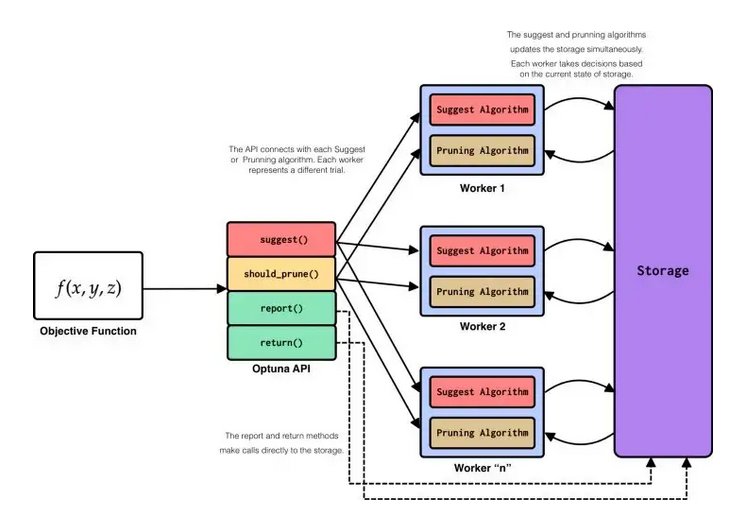
\includegraphics[scale=0.3]{images/arquitetura_optuna.png}
\end{figure}

\section{\textit{SHAP e Shapley Values}}
Entender a importância das variáveis de um modelo predito é um conceito extremamente necessário e importante. As variáveis podem explicar a dinâmica do problema no mundo real, que em muitos casos são desconhecidas, aprimorando o conhecimento do 
 do problema para o cientista de dados ou pesquisadores envolvidos na construção do modelo. Também podem ser usadas para auditar modelos complexos e entender se o modelo não está discriminando algo errado \cite{article:tec:interpr}.

 Essa tarefa é extremamente complexa, pois como vimos os modelos que vamos utilizar neste estudo, GBMs, fazem diversas operações no conjunto de dados, inclusive operações não-lineares. Isso torna a quantificação da importância de cada variável extremamente complexa.

\textit{SHAP (SHapley Additive exPlanations)} é uma abordagem que vem da teoria de jogos para explicar a saída de qualquer modelo de aprendizado de máquina. Ele conecta a saída do modelo com as explicações locais usando os valores de Shapley. A principal ideia do SHAP é criar um modelo mais simples, para que se possa explicar as como as variáveis locais impactam no modelo final \cite{shap:article,shap:article2,shap:doc}.

\begin{figure}[H]
 \caption{Exemplo do SHAP mostrando a importância de cada variável de entrada na saída do modelo \cite{shap:doc}.}
 \label{fig:ex:shap}
 \centering
 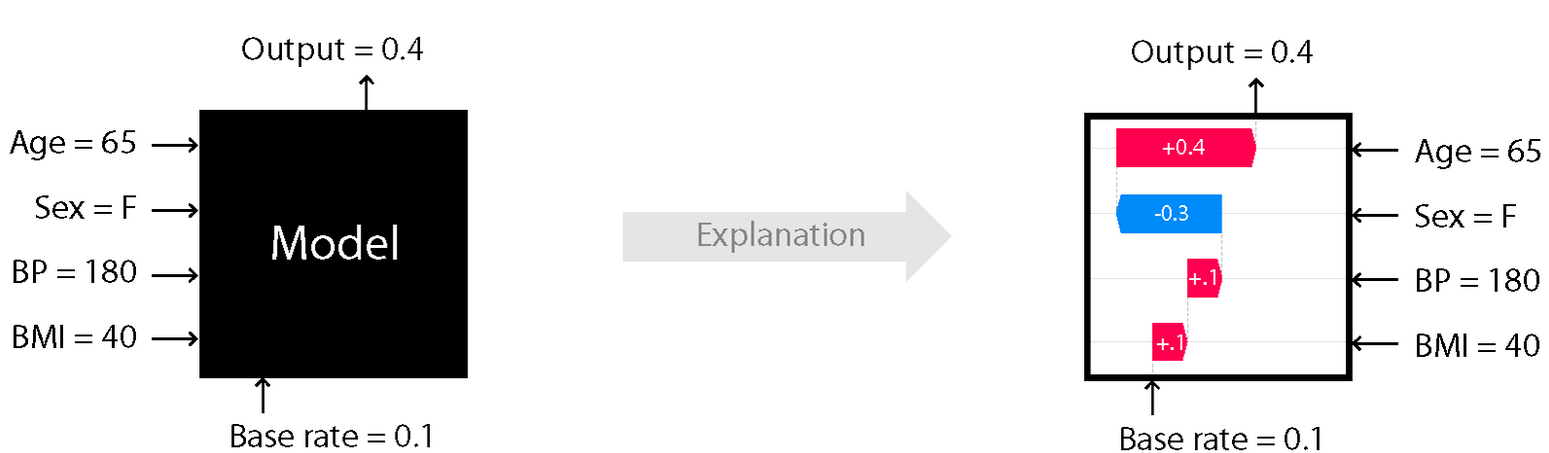
\includegraphics[scale=0.2]{images/exemplo_shap_black.png}
\end{figure}

\begin{figure}[H]
 \caption{Esquemático de como usar o SHAP para interpretar as predições do modelo \cite{iee:artigo:shap}}.
 \label{fig:ex:shap2}
 \centering
 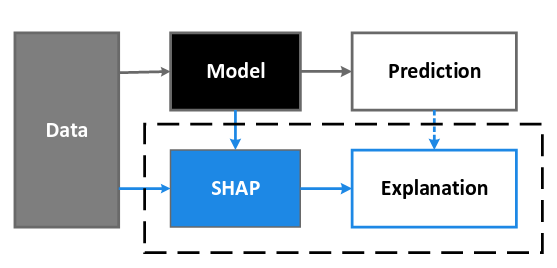
\includegraphics[scale=0.4]{images/over_shap.png}
\end{figure}

Estes métodos têm um modelo de explicação que é uma função linear de variáveis binárias:

\begin{equation}
    g(z') = \phi_{0} + \sum_{i=1}^{M} \phi_{i}z'_{i}
\end{equation}

Em que $z'\in \{0,1\}^M$, $M$ é o número de características de entrada simplificada e $\phi_i\in\mathbb{R}$. Os métodos atribuem um efeito $\phi_i\in\mathbb{R}$ a cada variável e a soma de todos os efeitos se aproxima do modelo original que queremos explicar. Uma das maiores contribuições do SHAP é propor a sua própria lógica de computar estes valores que garantem que eles tenham outras propriedades interessantes além do seu somatório aproximar a resposta do modelo original. E toda esta lógica surge dos \textit{Shapley Values}.


Os \textit{Shapley Values} foram introduzidos por Lloyd Shapley, no contexto da teoria dos jogos. Para um jogo cooperativo qualquer, os \textit{Shapley Values} distribuem uma quantidade total de contribuição para cada jogador da equipe de forma justa, ou seja tenta quantificar a contribuição individual para o ganho total \cite{shapley}. Em aprendizado de máquina, os valores de Shapley são a contribuição média de um valor de feature para a previsão total \cite{iee:artigo:shap}.

\begin{equation}
    \phi_i(f,x') = \sum_{z'\subseteq x'} \frac{|z'|!(M-|z'|-1)!}{M!}[f_x(z')-f_x(z'\setminus i)]
\end{equation}

\begin{figure}[H]
 \caption{SHAP valores atribuem a cada feição a mudança na previsão do modelo esperado ao condicionar esse recurso. Eles explicam como chegar do valor base $E[f (z)]$ que seria previsto se não conhecêssemos nenhum recurso para a saída atual $f(x)$. Este diagrama mostra um único pedido. Quando o modelo é não linear ou as características de entrada são não independentes, no entanto, a ordem em que os recursos são adicionados à expectativa importa, e os valores SHAP surgem da média dos valores $\phi_i$ em todas as ordenações possíveis. \cite{shap:article}}.
 \label{fig:ex:shap2}
 \centering
 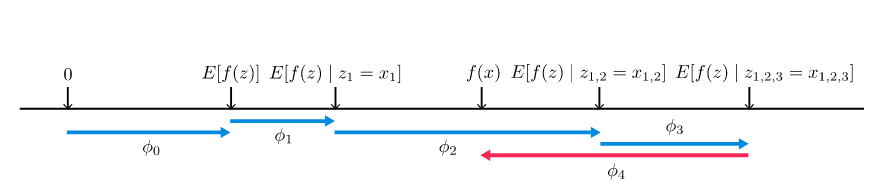
\includegraphics[scale=0.4]{images/shap_value_artigo.png}
\end{figure}

\begin{figure}[H]
 \caption{Gráfico do SHAP para o dataset Boston Housing.}.
 \label{fig:ex:shap_housing}
 \centering
 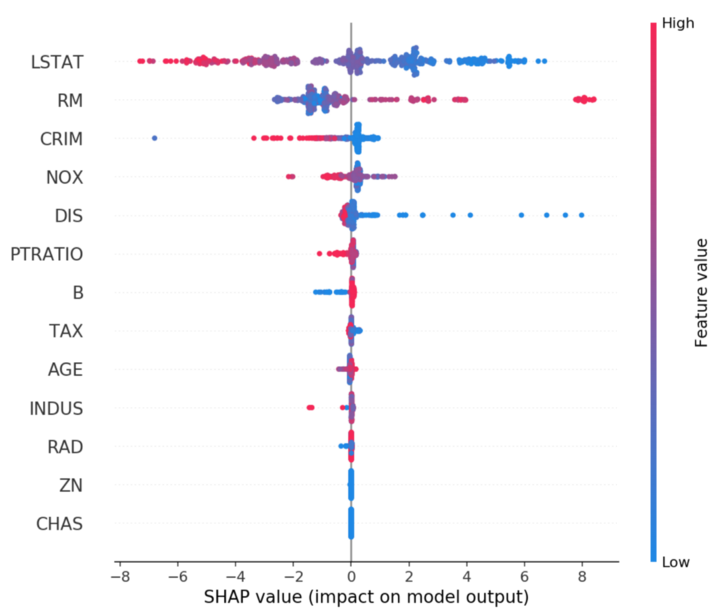
\includegraphics[scale=0.4]{images/shap_example_house.png}
\end{figure}



\chapter{Desenvolvimento}
\label{chapter:desenvolvimento}

\label{cap:desen}
O principal objetivo deste trabalho é estudar e comparar os algoritmos de boosting em 4 datasets diferentes e analisar a influência dos hiperparâmetros no modelo. O estudo será feito com os parâmetros \textit{Default} de cada algoritmo, depois alguns deles serão alterados e, por final, utilizaremos o Optuna para otimizá-los.

O objetivo da escolha dos conjuntos de dados se baseou em analisar o comportamento dos modelos construídos e dos hiperparâmetros em conjuntos de dados com propriedades distintas, como por exemplo maior presença de variáveis categóricas ou apenas variáveis numéricas.

Nas próprias seções, será abordada uma visão geral da metodologia, uma análise dos conjuntos de dados e as implementações no \textit{jupyter-notebook}.

\section{Bibliotecas e Ferramentas}
Todo o pipeline de estudo e análise é feito usando Python 3.8.8. No código final no GitHub será detalhado todas as versões em um arquivo \textit{requeriments.txt}, mas de modo geral as principais bibliotecas utilizadas nesse estudo são:
\begin{itemize}
    \item \textbf{numpy:} biblioteca em python para trabalhar com arrays n-dimensional e algumas funções matemáticas de álgebra linear.
    \item \textbf{pandas:} biblioteca em python utilizada para manipulação e análise de conjunto de dados e séries temporais.
    \item \textbf{matplotlib:} biblioteca em python para visualização de dados.
    \item \textbf{seaborn:} biblioteca em python para visualização de dados baseada no \textbf{matplotlib:}.
    \item \textbf{scipy:} biblioteca em python de pacote científico computacional
    \item \textbf{sys:} biblioteca que oferece funções e variáveis usadas para manipular diferentes partes do ambiente e do tempo de execução do python.
    \item \textbf{timeit:} biblioteca para medir o tempo de execução de programas python.
    \item \textbf{gc:} é o garbage collector utilizado nas linguagens de programação para rastrear os objetos na memória.
    \item \textbf{sklearn:} biblioteca de aprendizado de máquina em python.
    \item \textbf{xgboost:} biblioteca do XGBoost.
    \item \textbf{catboost:} biblioteca do CatBoost.
    \item \textbf{lightbm:} biblioteca do LightGBM.
    \item \textbf{optuna:} biblioteca do Optuna.
    \item \textbf{shap:} biblioteca do SHAP.
\end{itemize}

\section{Data Cleaning, Data Preparation e Análise Descritiva}
Nesta seção iremos fazer uma breve descrição dos conjuntos de dados, análise descritivas das variáveis e a distribuição nos conjuntos de dados. Primeiramente, precisamos ajustar dados que foram inseridos incorretamente, lidar com os valores \textit{missing} e realizar as transformações, ou conversões, das variáveis para cada modelo, por exemplo variáveis categóricas para numéricas no caso do LightGBM e XGBoost. 
Todas as análises nos conjunto de dados seguem a mesma metodologia: identificar o tipo de cada coluna (int, float, str) verificar se existem valores \textit{missing} e realizar as transformações ou criações de variáveis para cada modelo.

Serão utilizados 4 conjunto de dados diferentes para este estudo, todos eles podem ser encontrados no \href{https://www.openml.org/}{OpenML}, \href{https://www.kaggle.com/}{Kaggle} ou \href{https://archive.ics.uci.edu/ml/index.php}{UCI Machine Learning Repository}. 
\subsection{Diabetes}
O primeiro conjunto de dados é o \href{https://www.kaggle.com/datasets/tigganeha4/diabetes-dataset-2019}{Diabetes Dataset 2019}
Este conjunto de dados é originalmente do \textit{Prediction of Type 2 Diabetes using Machine Learning Classification Methods}. O objetivo é prever, com base em medidas de diagnóstico, se um paciente tem diabetes. As variáveis são:
\begin{itemize}
    \item \textbf{Idade:} idade faixa de anos.
    \item \textbf{Sexo:} sexo do paciente [M: Masculino, F: Feminino].
    \item \textbf{Diabetes na Família:} se tem diabetes no histórico familiar.
    \item \textbf{Pressão Alta:} se o paciente possui pressão alta.
    \item \textbf{Atividade Física:} se pratica atividade física.
    \item \textbf{IMC:} índice de massa corporal (peso em $kg$/(altura em $m$)$^2$).
    \item \textbf{Fumante:} indica se o paciente é fumante.
    \item \textbf{Alcoólatra:} indica se o paciente é alcoólatra.
    \item \textbf{Horas de sono:} quantidade de horas de sono
    \item \textbf{Sono Profundo:} horas de sono profundo.
    \item \textbf{Medicamentos Regulares:} indica se o paciente utiliza medicamentos
    \item \textbf{JunkFood:} se o paciente consome comidas gordurosas.
    \item \textbf{Stress:} stress do paciente.
    \item \textbf{BPLevel:} nível da pressão arterial.
    \item \textbf{Gravidezes:} número de gravidezes.
    \item \textbf{Pdiabetes:} se possui pré-diabetes.
    \item \textbf{Frequência Urinaria:} frequência urinaria.
    \item \textbf{Resultado:} variável alvo (0 ou 1), se possui ou não possui diabete.
    
\end{itemize}
O primeiro passo é identificar o nome de cada coluna, seus atributos e os valores \textit{NaN} em cada linha de cada coluna. E para as variáveis numéricas uma análise descritiva, média, desvio padrão, contagem, mínimo e máximo e os quantis (25,50,75).
 
\begin{table}[H]
\begin{subtable}[c]{0.5\textwidth}
\label{descritivo:diabete}
\centering
\begin{tabular}{|c|c|c|}
 \hline
\textbf{Coluna} & \textbf{dtypes} & \textbf{\textit{NaN}}\\
  \hline
Age                &  object & 0\\
\hline
Gender             &  object & 0\\
\hline
Family\_Diabetes   &   object & 0 \\
\hline
highBP             &  object & 0 \\
\hline
PhysicallyActive   &  object & 0 \\
\hline
BMI                & float64 & 4 \\
\hline
Smoking            &  object & 0 \\
\hline
Alcohol            &  object & 0 \\
\hline
Sleep              &   int64 & 0 \\
\hline
SoundSleep         &   int64 & 0 \\
\hline
RegularMedicine    &  object & 0 \\
\hline
JunkFood           &  object & 0 \\
\hline
Stress             &  object & 0 \\
\hline
BPLevel            &  object & 0 \\
\hline
Pregancies         & float64 & 42 \\
\hline
Pdiabetes          &  object & 1 \\
\hline
UriationFreq       &  object & 0 \\
\hline
Diabetic           &  object & 1 \\
\hline
\end{tabular}
\subcaption{Tabela com o tipo de cada variável e quantidade de linhas \textit{NaN} em cada coluna.}
\end{subtable}
\begin{subtable}[c]{0.5\textwidth}
\centering
\begin{tabular}{|c|c|c|c|c|}
\hline
	& \textbf{BMI}	& \textbf{Sleep}	& \textbf{SoundSleep}	& \textbf{Pregancies}\\
\hline
\textbf{count}	& 948	& 952	& 952	& 910 \\
\hline
\textbf{mean}	& 25.7637	& 6.9495	& 5.4957	& 0.3868 \\
\hline
\textbf{std}	    & 5.4025	& 1.2731	& 1.8656	& 0.9094 \\
\hline
\textbf{min}	    & 15	& 4	& 0	& 0 \\
\hline
\textbf{25\%}	& 22	& 6	& 4	& 0 \\
\hline
\textbf{50\%}	& 25	& 7	& 6	& 0 \\
\hline
\textbf{75\%}	& 29	& 8	& 7	& 0 \\
\hline
\textbf{max}	    & 45	& 11	& 11	& 4 \\
\hline
\end{tabular}
\subcaption{Estatística descritiva das variáveis numéricas.}
\end{subtable}
\caption{Descritivo das variáveis no conjunto de dados Diabetes.}
\end{table}

Precisamos realizar um tratamento nessas linhas com \textit{NaN} e na variável resposta, Diabetic, transformando ela em 0 ou 1. Após isso devemos conferir as variáveis categorias estão escritas corretamente e podemos analisar a distribuição de algumas variáveis na população com diabete e sem diabete.


\begin{figure}[H]
 \caption{População com Diabetes e sem Diabetes.}.
 \label{fig:pop:targ:dia}
 \centering
 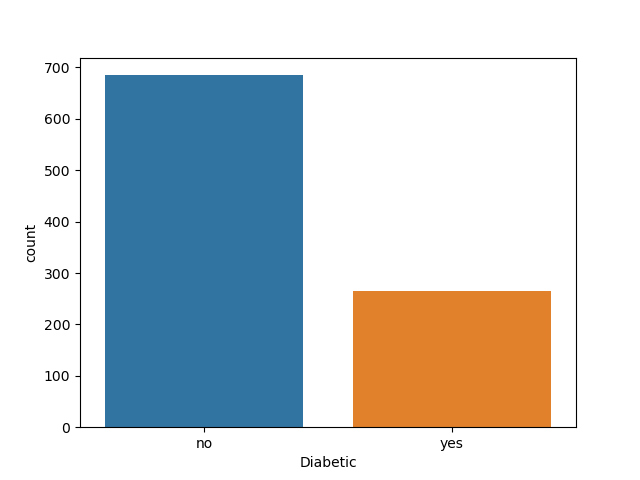
\includegraphics[scale=0.4]{images/diabete_tot.png}
\end{figure}


\begin{figure}[H]
 \caption{Distribuição das Variáveis categóricas no conjunto de dados de Diabetes.}
 \label{fig:var:cat:1:diab}
 \centering
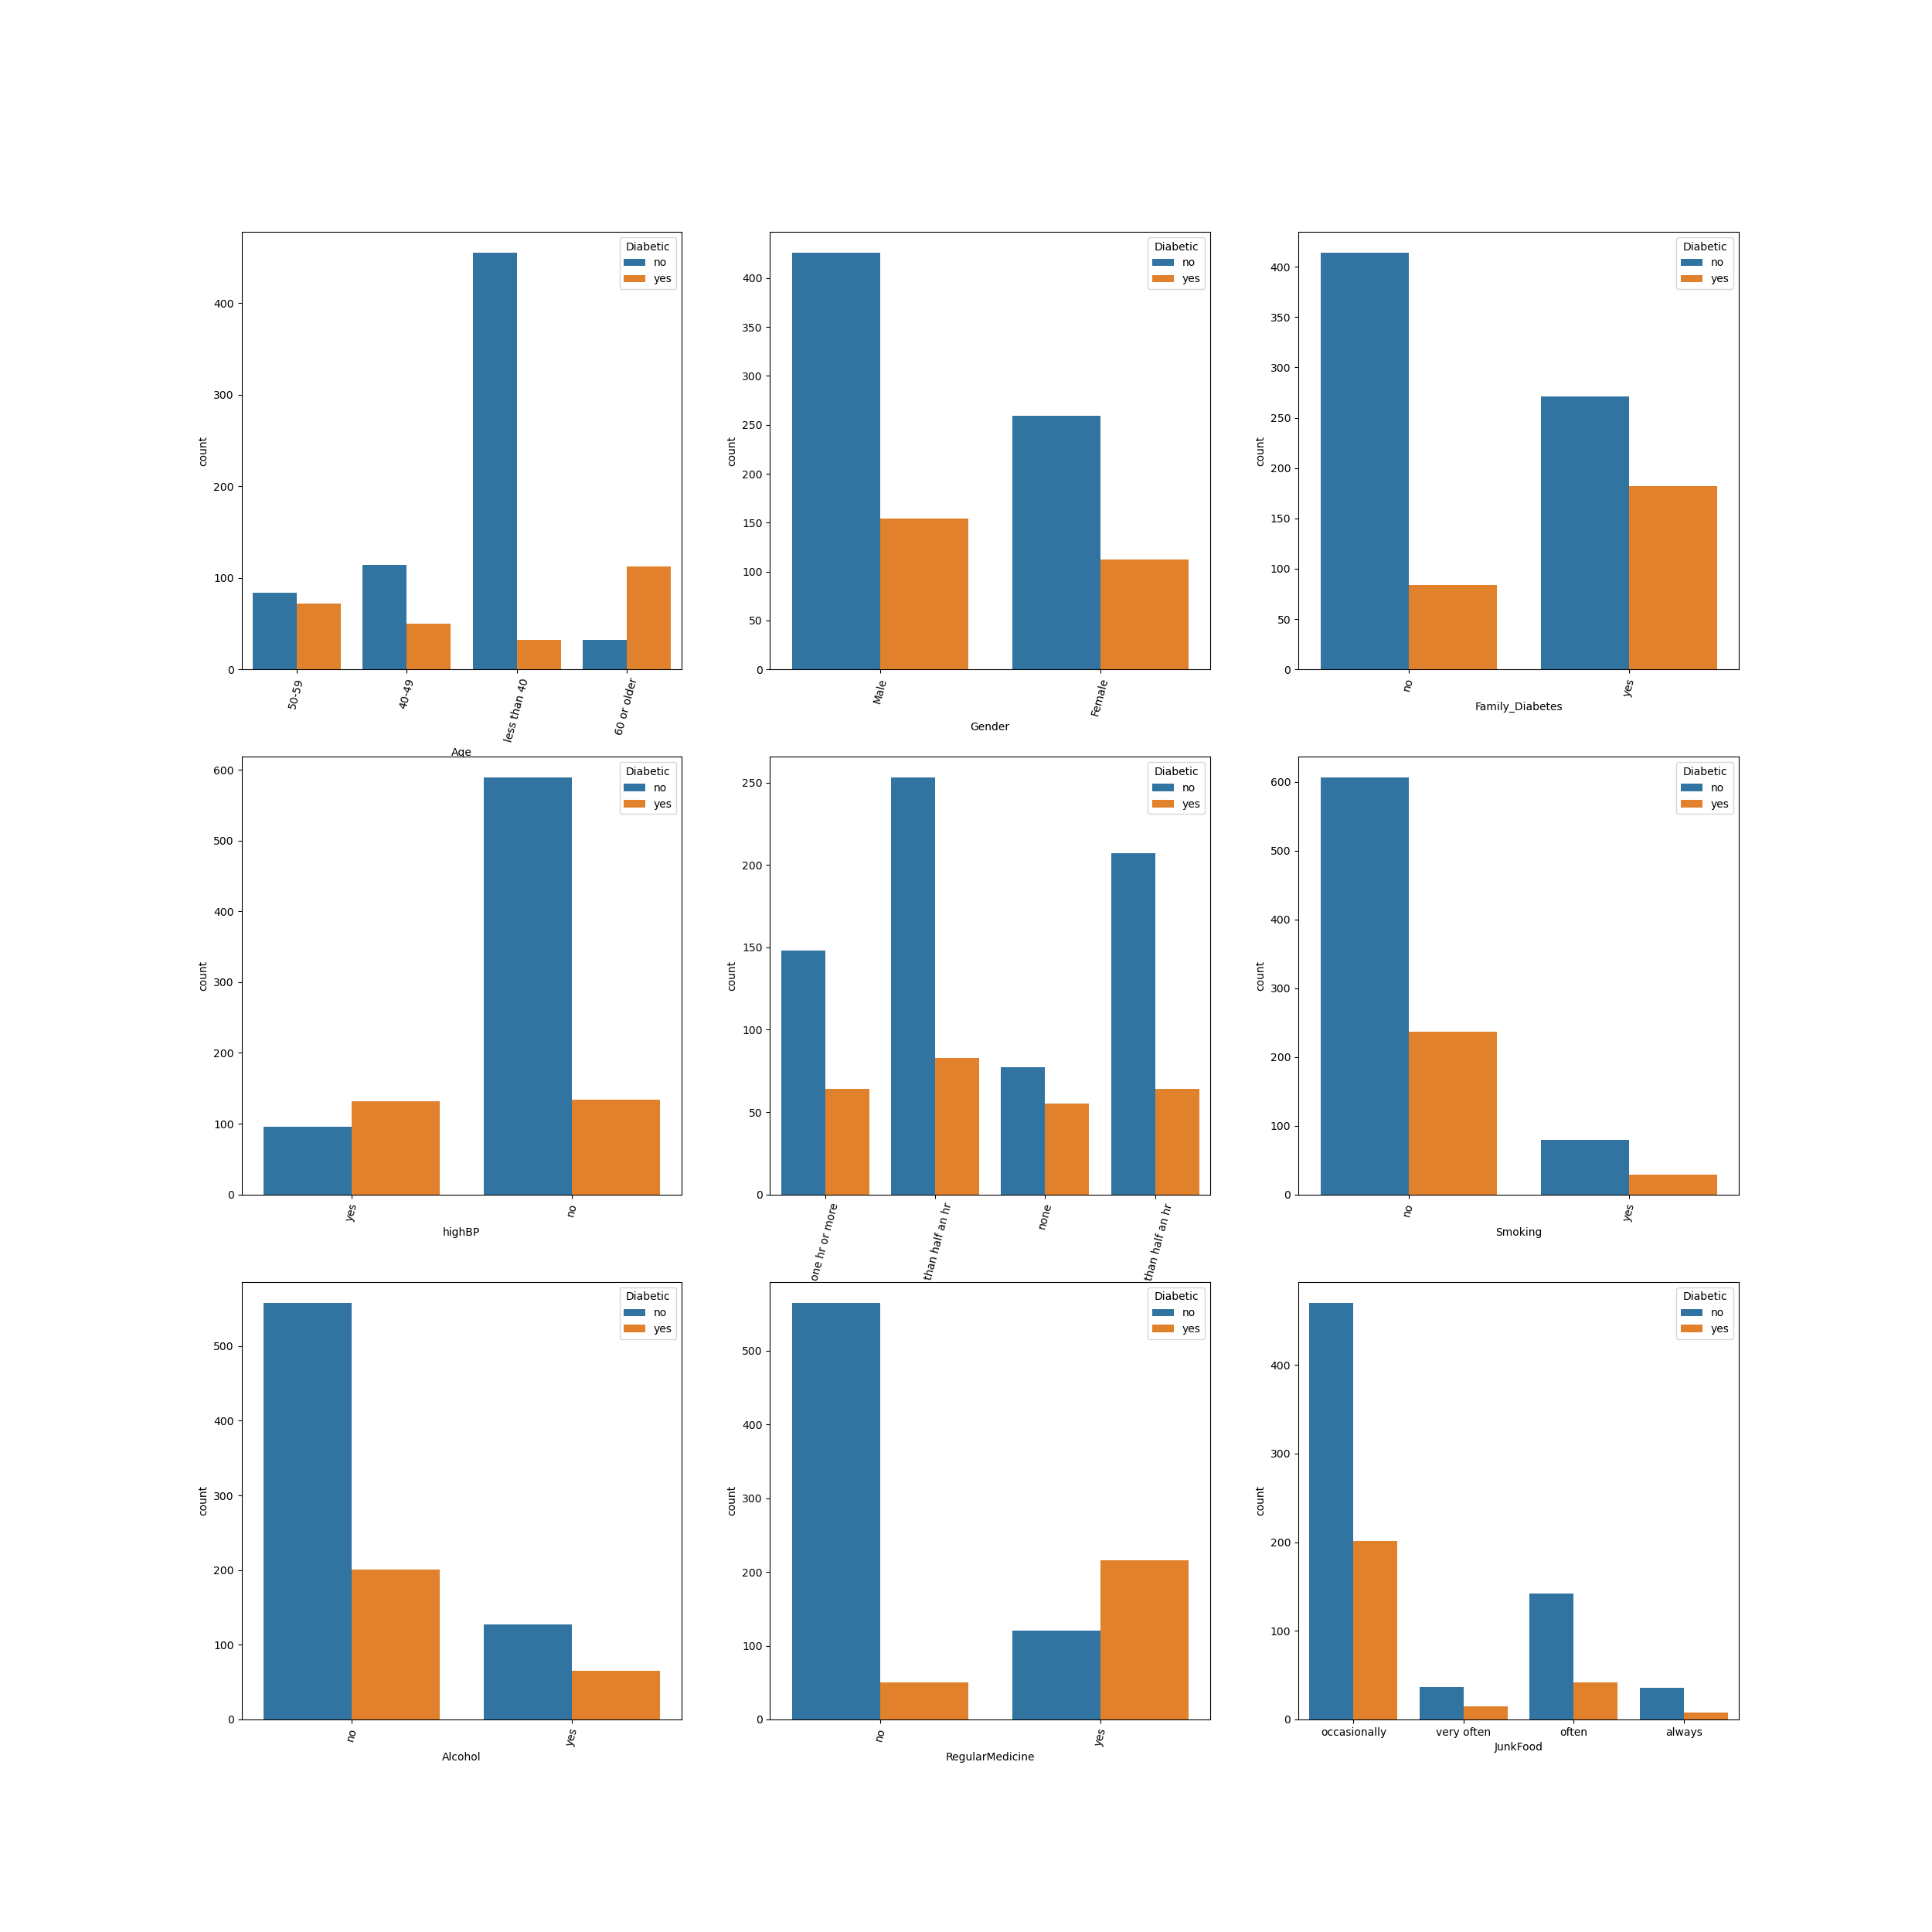
\includegraphics[scale=0.2]{images/diabete_desc.png}
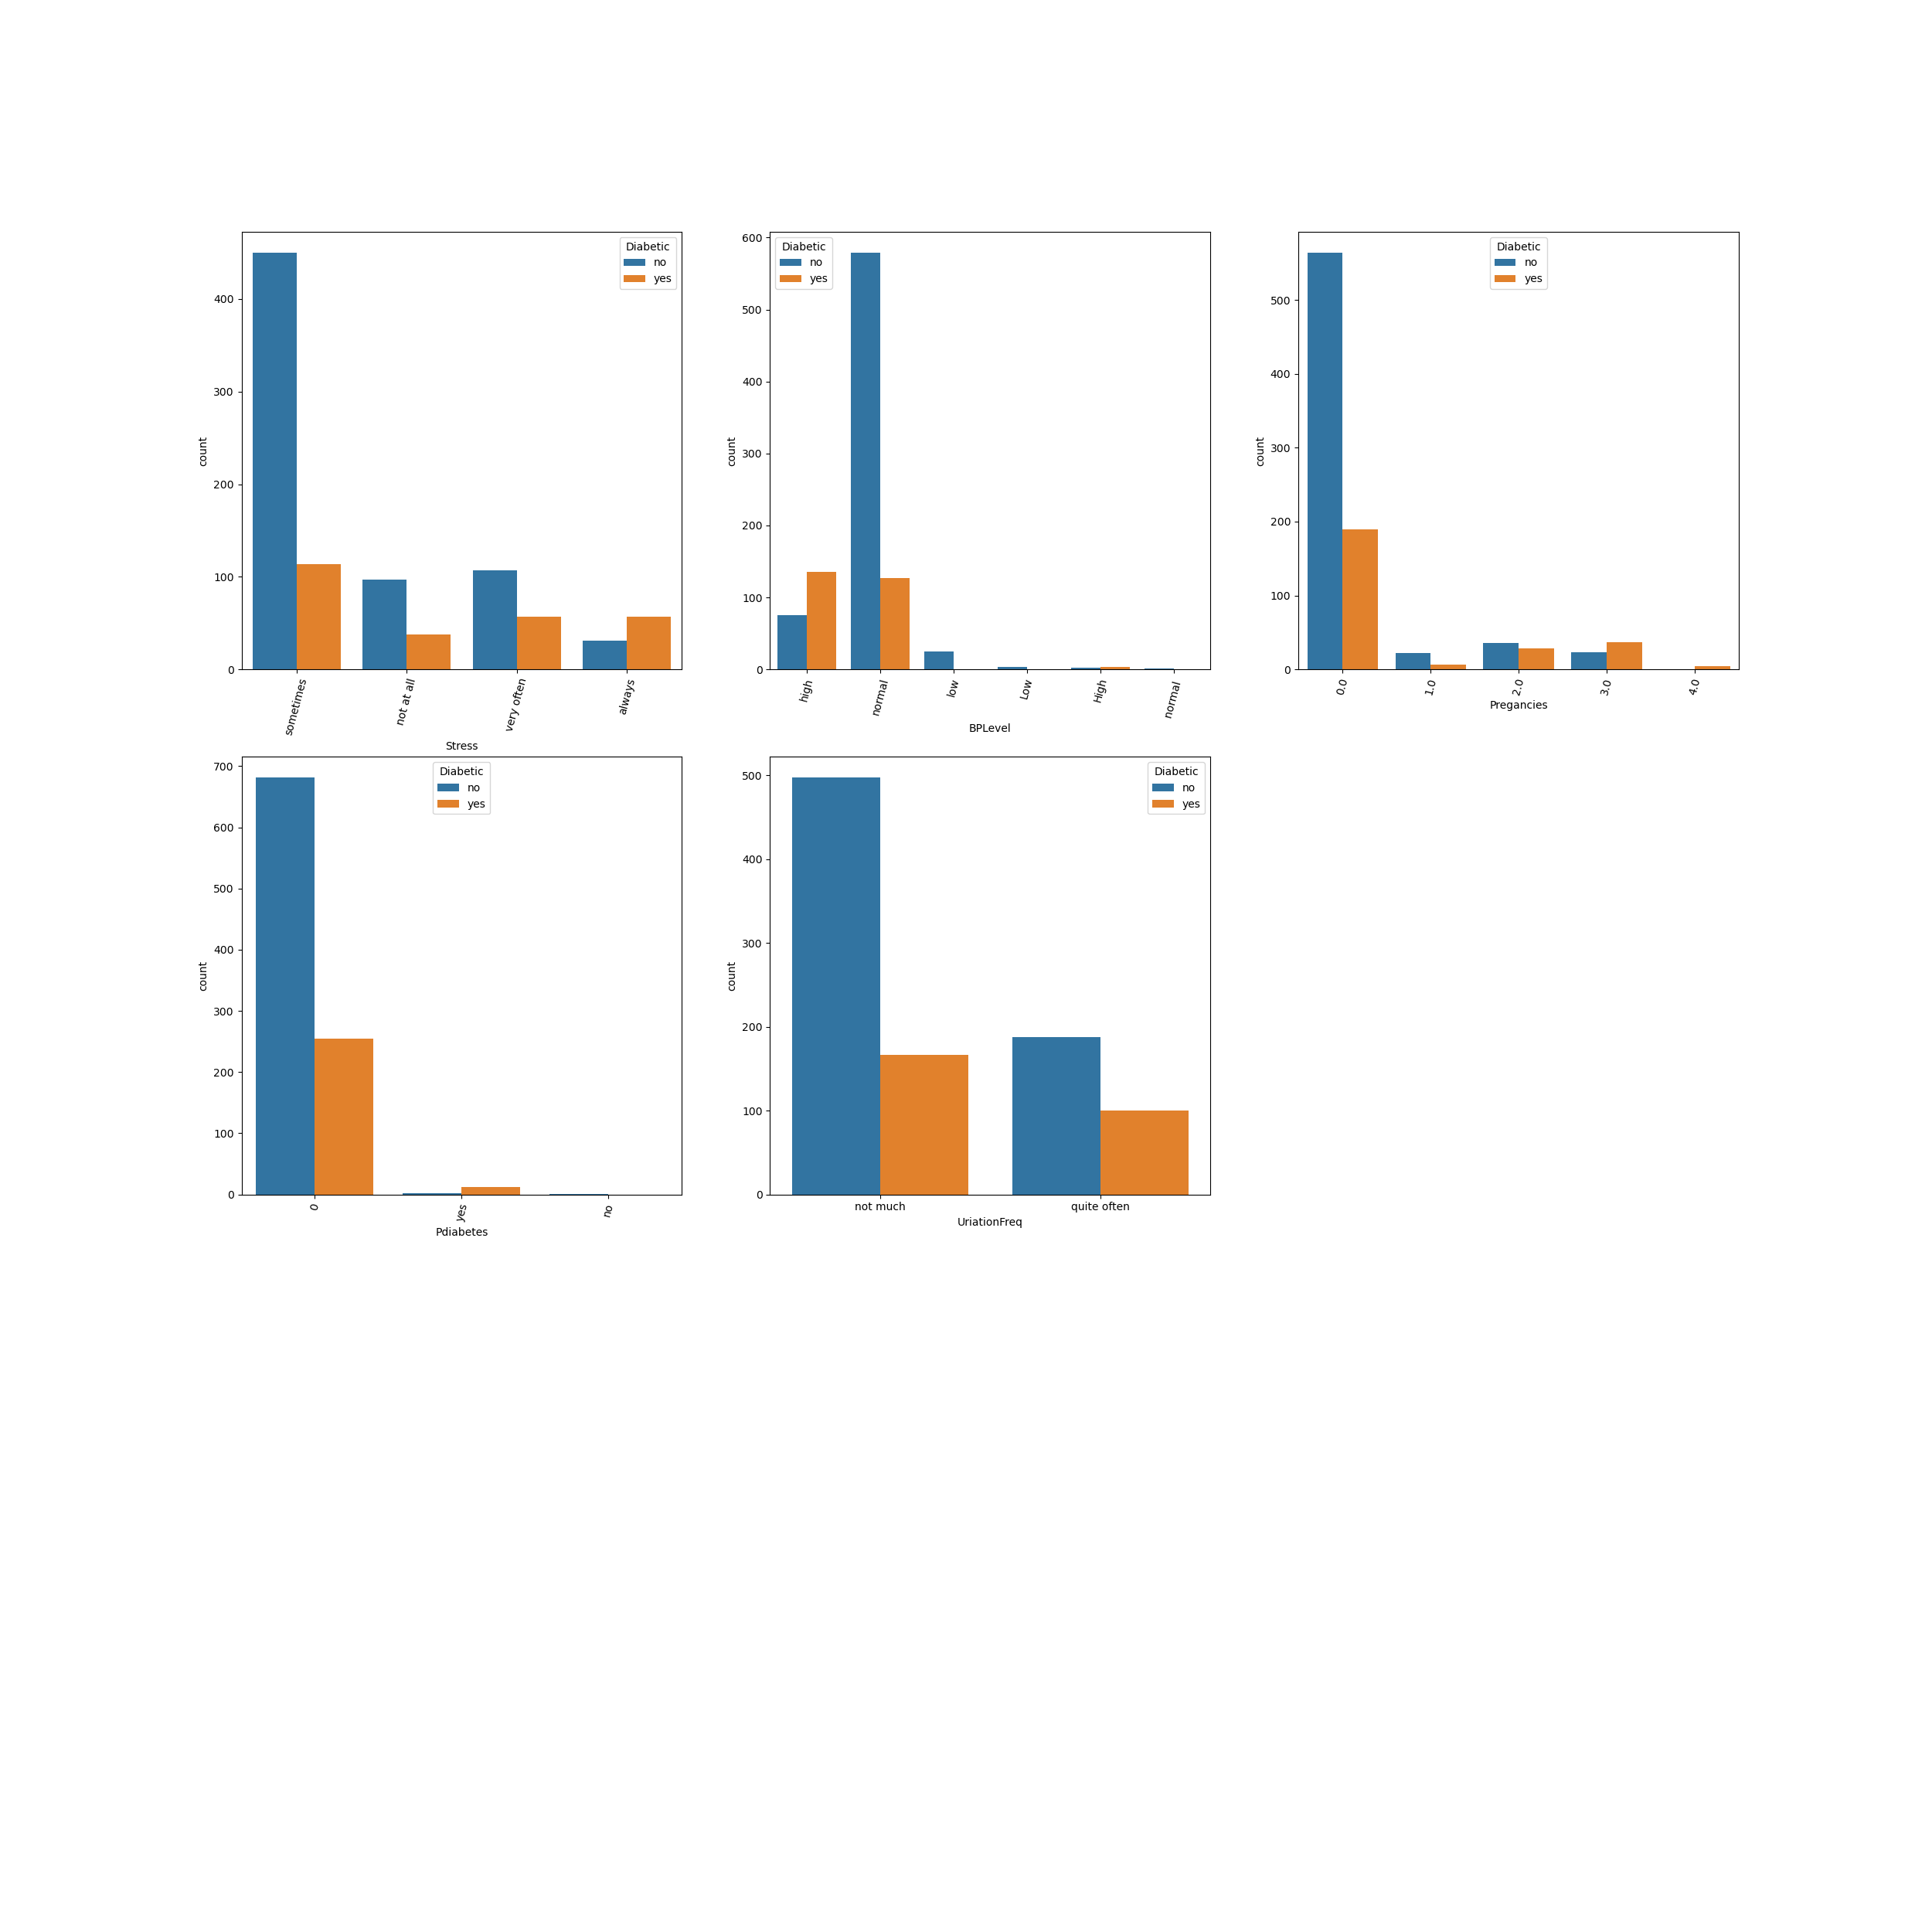
\includegraphics[scale=0.2]{images/diabete_desc_2.png}
\end{figure}


\begin{figure}[H]
     \centering
     \begin{subfigure}[b]{0.3\textwidth}
         \ \caption{Histograma das variáveis numéricas na população total.}
 \label{fig:var:1:diab}
 \centering
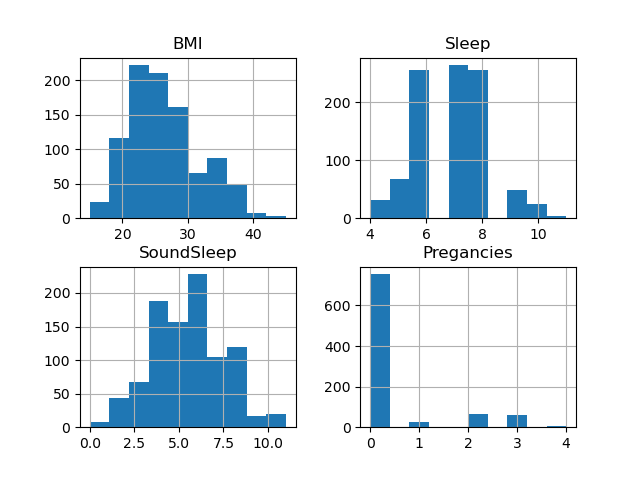
\includegraphics[scale=0.3]{images/hist_diabete.png}
     \end{subfigure}
     \hfill
     \begin{subfigure}[b]{0.3\textwidth}
         \centering
         \caption{Histograma das variáveis numéricas na população com Diabete.}
 \label{fig:var:2:diab}
 \centering
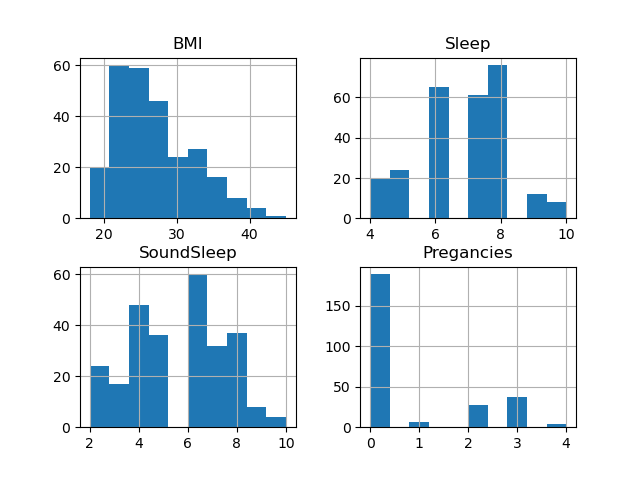
\includegraphics[scale=0.3]{images/hist_diabete_yes.png}
     \end{subfigure}
     \hfill
     \begin{subfigure}[b]{0.3\textwidth}
 \caption{Histograma das variáveis numéricas na população sem Diabete.}
 \label{fig:var:3:diab}
 \centering
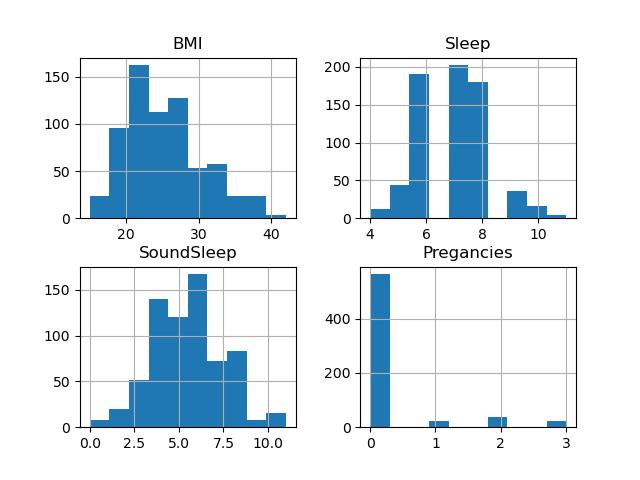
\includegraphics[scale=0.3]{images/hist_diabete_no.png}
     \end{subfigure}
        \caption{Distribuição das variáveis numéricas no conjunto de dados de Diabetes.}
         \label{fig:var:diab:t}
\end{figure}


A próxima etapa consistirá em dividir esse conjunto de dados em dois, o primeiro é com as próprias variáveis categóricas para o CatBoost enquanto que para o modelo do LightGBM e XGBoost iremos transformar as variáveis em ordinais ou utilizaremos \textit{one\_hot\_enconding}. A partir disto já teremos os nossos conjuntos de dados para o treinamento dos modelos.
\subsection{Insuficiência Cardíaca}
O segundo conjunto de dados é o \href{https://www.kaggle.com/datasets/fedesoriano/heart-failure-prediction}{Heart Failure Prediction Dataset}
Este conjunto de dados foi criado combinando diferentes conjuntos de dados já disponíveis de forma independente, mas não combinados antes. Neste conjunto de dados, 5 conjuntos de dados cardíacos são combinados em 11 características comuns. O objetivo é identificar a insuficiência cardíaca com base nas seguintes variáveis:
\begin{itemize}
    \item \textbf{Sexo:} sexo do paciente [M: Masculino, F: Feminino].
    \item \textbf{TipoDorPeito:} tipo de dor no peito.
    \item \textbf{Pressão arterial em repouso:} pressão arterial em repouso (mmHg).
    \item \textbf{Colesterol:} colesterol sérico[mm/dl]
    \item \textbf{JejumBS:} açúcar no sangue em jejum [1: se JejumBS > 120 mg/dl, 0: caso contrário].
    \item \textbf{ECG em repouso::} resultados do eletrocardiograma em repouso [Normal: Normal, ST: com anormalidade da onda ST-T (inversões da onda T e/ou elevação ou depressão do ST $>$ 0,05 mV).
    \item \textbf{HVE:} mostrando hipertrofia ventricular esquerda provável ou definitiva pelos critérios de Estes]
    \item \textbf{MaxHR:} frequência cardíaca máxima alcançada [Valor numérico entre 60 e 202].
    \item \textbf{ExerciseAngina:} angina induzida por exercício [S: Sim, N: Não].
    \item \textbf{Oldpeak:} oldpeak = ST [Valor numérico medido na depressão].
    \item \textbf{ST\_Slope:} a inclinação do segmento ST do exercício de pico [Up: ascendente, Flat: plano, Down: descendente].
    \item \textbf{Idade:} idade em anos.
    \item \textbf{Resultado:} variável alvo (0 ou 1), se possui ou não possui insuficiência cardíaca.
\end{itemize}

\begin{table}[H]
\label{descritivo:heart}
\centering
\begin{tabular}{|c|c|c|}
\hline
\textbf{Coluna} & \textbf{dtypes} & \textbf{\textit{NaN}}\\
\hline
Age              &   int64 & 0\\
\hline
Sex              &  object & 0\\
\hline
ChestPainType    &  object & 0\\
\hline
RestingBP        &   int64 & 0\\
\hline
Cholesterol      &   int64 & 0\\
\hline
FastingBS        &   int64 & 0\\
\hline
RestingECG       &  object & 0\\
\hline
MaxHR            &   int64 & 0\\
\hline
ExerciseAngina   &  object & 0\\
\hline
Oldpeak          & float64 & 0\\
\hline
ST\_Slope        &   object & 0\\
\hline
HeartDisease     &   int64 & 0\\
\hline
\end{tabular}
\caption{Tabela com o tipo de cada variável e quantidade de linhas \textit{NaN} em cada coluna no conjunto de dados de Insuficiência Cardíaca.}
\end{table}
\begin{table}[H]
\label{descritivo:heart2}
\centering
\begin{tabular}{|c|c|c|c|c|c|c|c|}
\hline
& \textbf{Age}	& \textbf{RestingBP}	& \textbf{Cholesterol}	& \textbf{FastingBS}	& \textbf{MaxHR}	& \textbf{Oldpeak}	& \textbf{HeartDisease} \\
 \hline
\textbf{count}	& 918.000	& 918.000	& 918.000	& 918.000	& 918.000	& 918.000	& 918.000 \\
 \hline
\textbf{mean}	& 53.511	& 132.397	& 198.800	& 0.233	& 136.809	& 0.887	& 0.553 \\
 \hline
\textbf{std}	    & 9.433	& 18.514	& 109.384	& 0.423	& 25.460	& 1.067	& 0.497 \\
 \hline
\textbf{min}	    & 28.000	& 0.000	& 0.000	& 0.000	& 60.000	& -2.600	& 0.000 \\
 \hline
\textbf{25\%}	& 47.000	& 120.000	& 173.250	& 0.000	& 120.000	& 0.000	& 0.000 \\
 \hline
\textbf{50\%}	& 54.000	& 130.000	& 223.000	& 0.000	& 138.000	& 0.600	& 1.000 \\
 \hline
\textbf{75\%}	& 60.000	& 140.000	& 267.000	& 0.000	& 156.000	& 1.500	& 1.000 \\
 \hline
\textbf{max}	    & 77.000	& 200.000	& 603.000	& 1.000	& 202.000	& 6.200	& 1.000 \\
\hline
\end{tabular}
\caption{Estatística descritiva das variáveis numéricas no conjunto de dados de Insuficiência Cardíaca.}
\end{table}
Neste conjunto de dados não precisamos fazer nenhum tratamento, pois os valores foram inseridos corretamente e não temos \textit{missing}.
\begin{figure}[H]
 \caption{População com Insuficiência Cardíaca e sem Insuficiência Cardíaca.}.
 \label{fig:pop:targ:card}
 \centering
 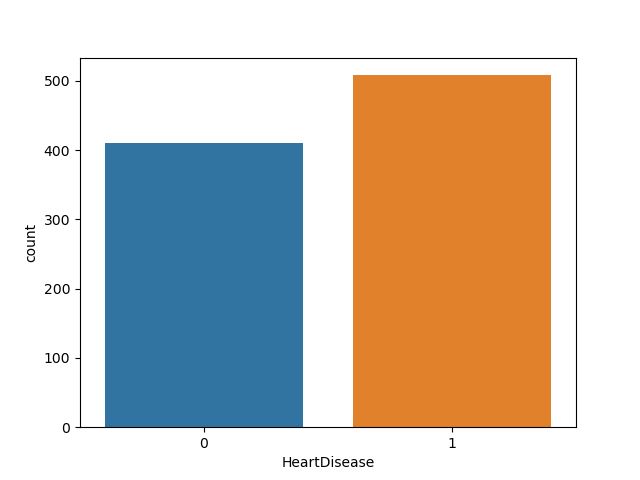
\includegraphics[scale=0.3]{images/heart_tot.png}
\end{figure}


\begin{figure}[H]
 \caption{Distribuição das variáveis categóricas no conjunto de dados de Insuficiência Cardíaca.}
 \label{fig:var:cat:1:card}
 \centering
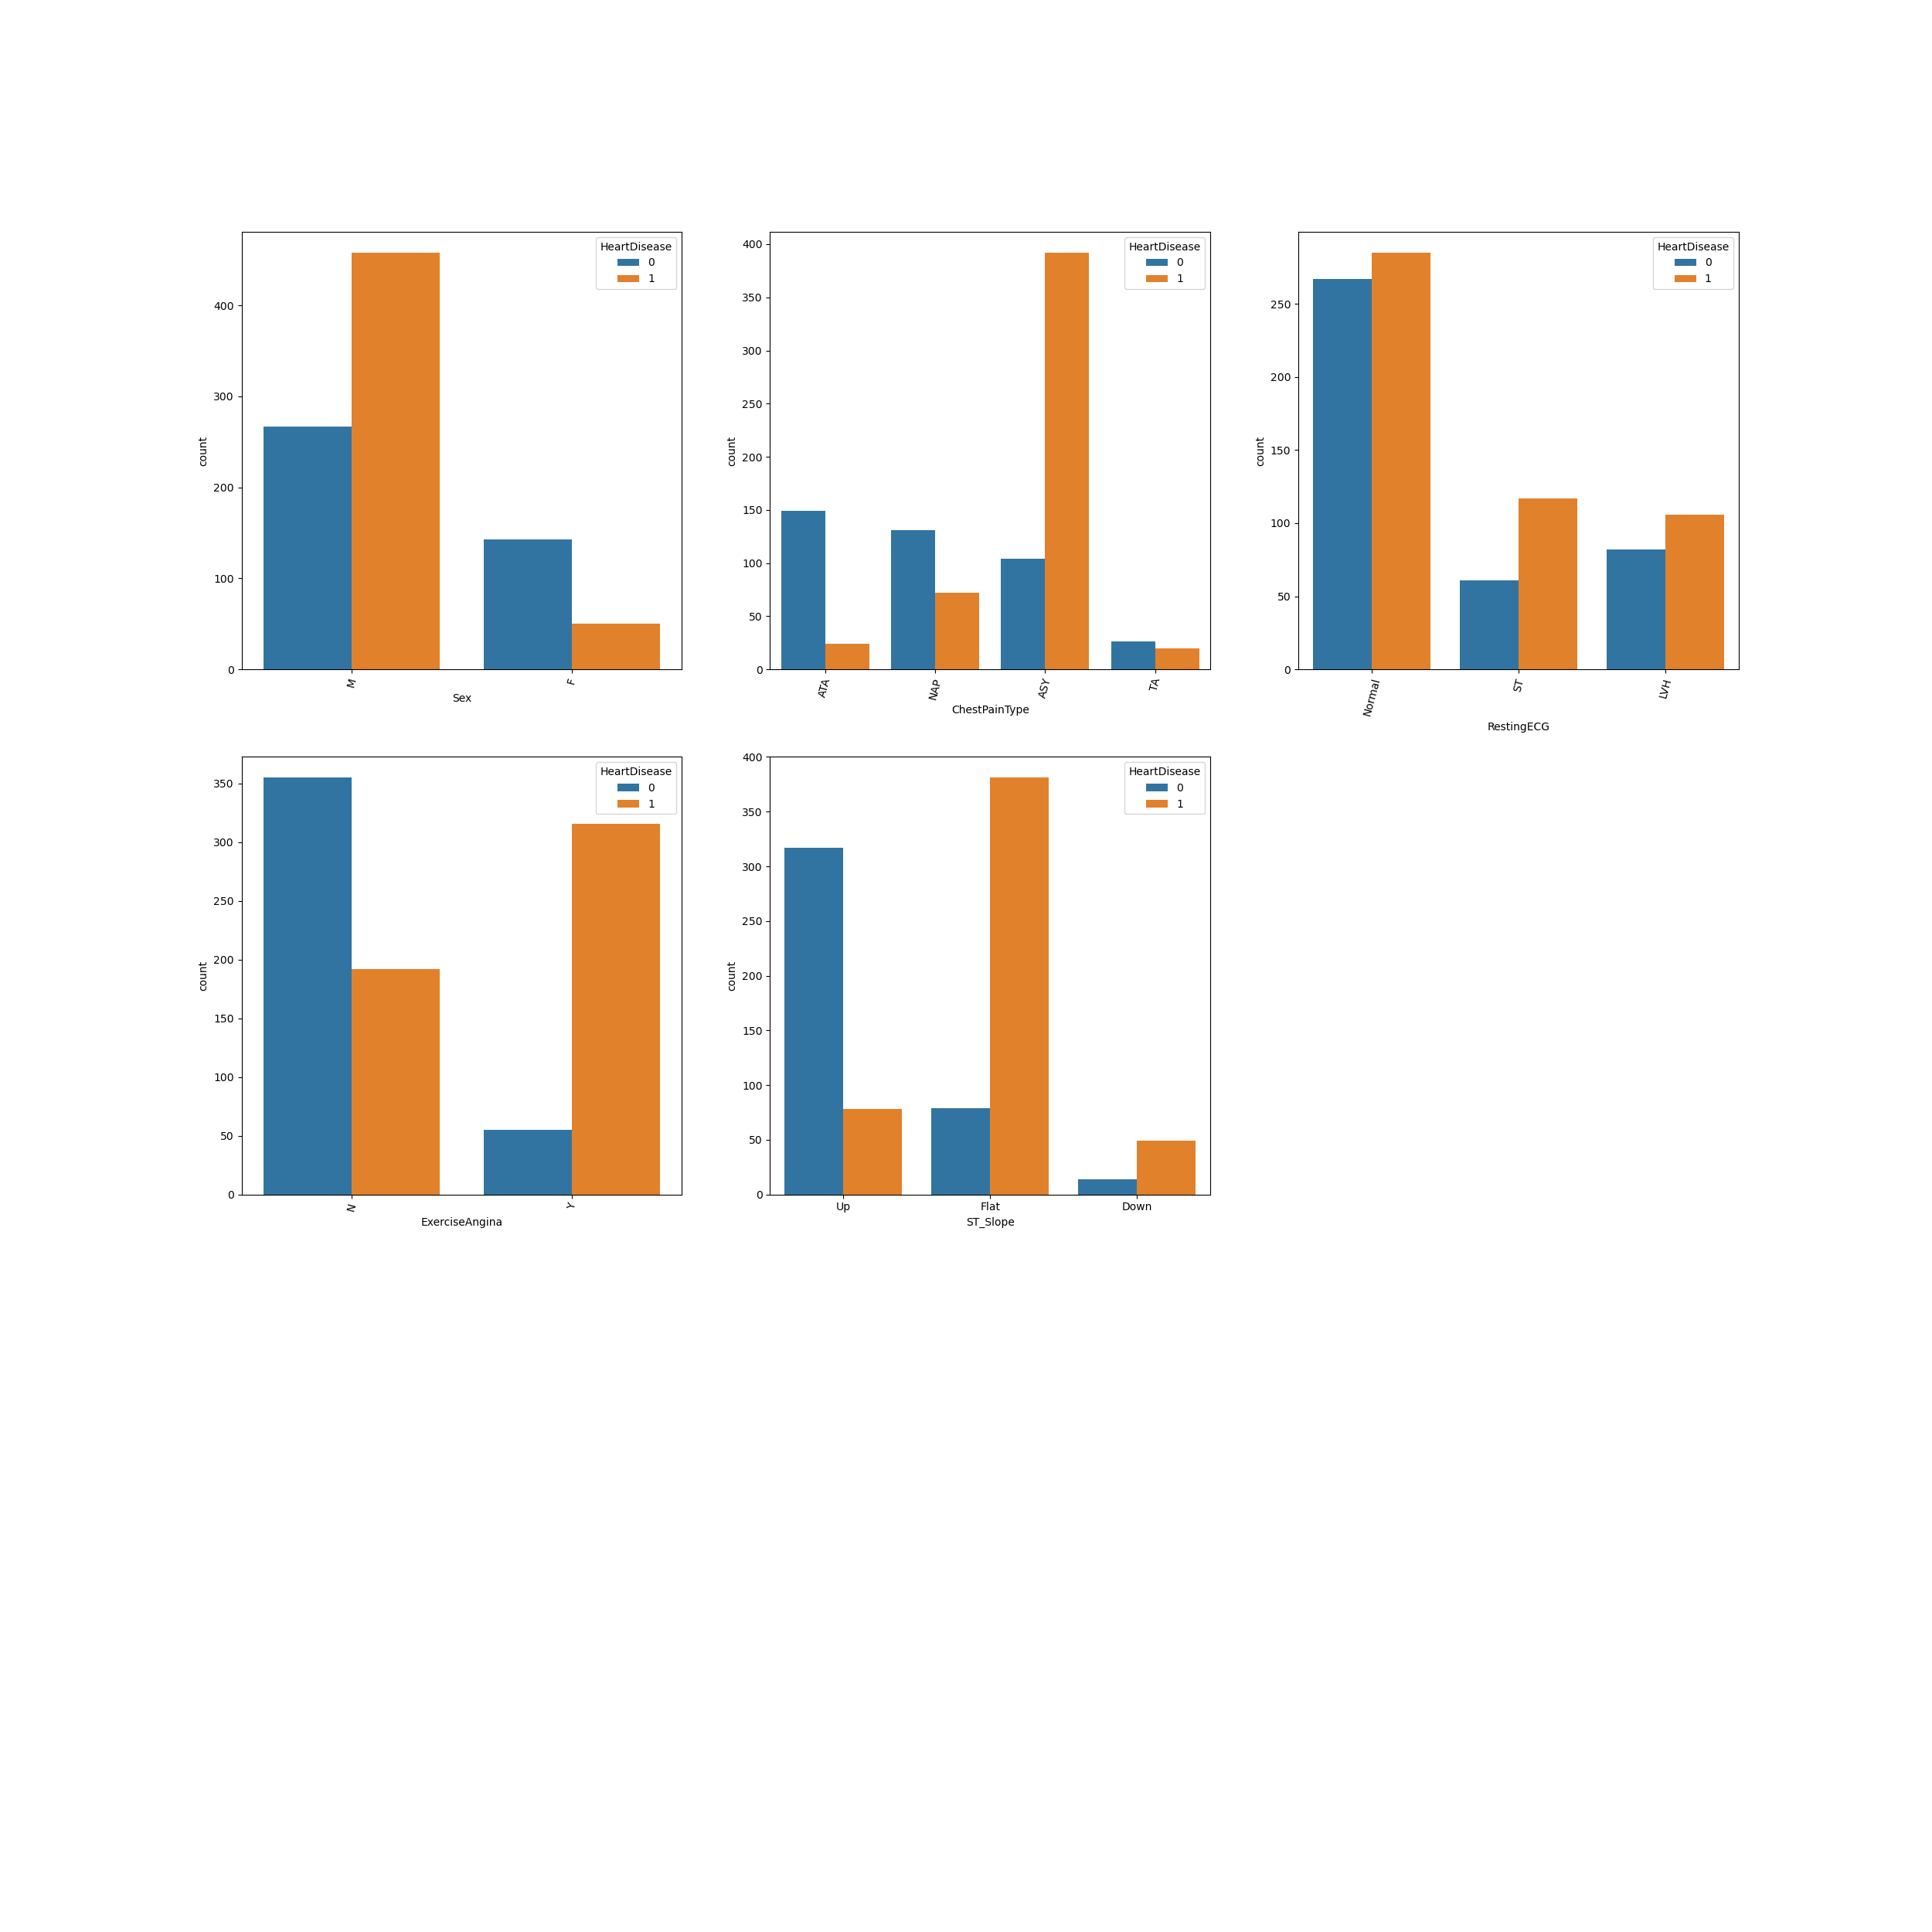
\includegraphics[scale=0.25]{images/heart_cat.png}
\end{figure}


\begin{figure}[H]
     \centering
     \begin{subfigure}[b]{0.3\textwidth}
         \ \caption{Histograma das variáveis numéricas na população total.}
 \label{fig:var:1:card}
 \centering
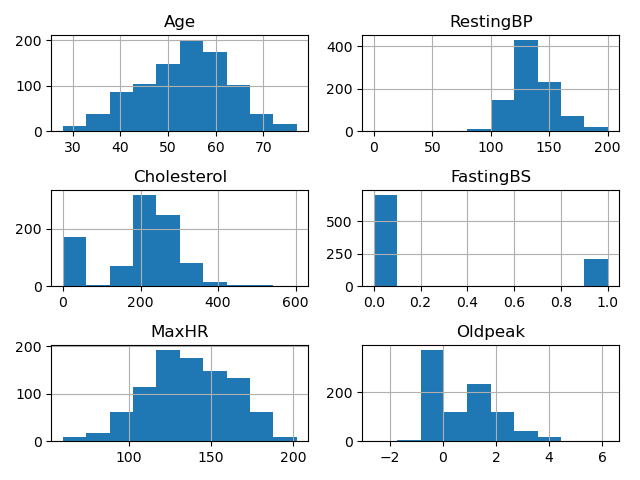
\includegraphics[scale=0.3]{images/hist_heart_t.png}
     \end{subfigure}
     \hfill
     \begin{subfigure}[b]{0.3\textwidth}
         \centering
         \caption{Histograma das variáveis numéricas na população com Insuficiência Cardíaca.}
 \label{fig:var:2:card}
 \centering
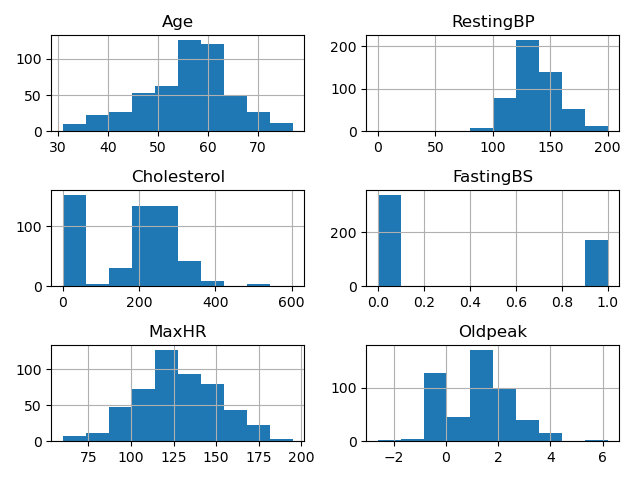
\includegraphics[scale=0.3]{images/hist_heart_yes.png}
     \end{subfigure}
     \hfill
     \begin{subfigure}[b]{0.3\textwidth}
 \caption{Histograma das variáveis numéricas na população sem Insuficiência Cardíaca.}
 \label{fig:var:3:card}
 \centering
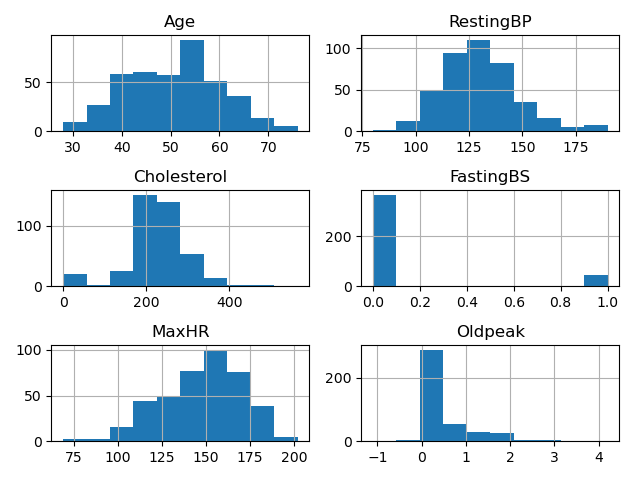
\includegraphics[scale=0.3]{images/hist_heart_no.png}
     \end{subfigure}
        \caption{Distribuição das variáveis numéricas no conjunto de dados de Insuficiência Cardíaca.}
         \label{fig:var:card:t}
\end{figure}

Neste caso iremos transformar as colunas categóricas em ordinais para o conjunto de treinamento nos modelos XGBoost e LightGBM.

\subsection{Cálculo Renal}
O terceiro conjunto de dados é o \href{https://www.kaggle.com/datasets/vuppalaadithyasairam/kidney-stone-prediction-based-on-urine-analysis}{Kidney Stone Prediction based on Urine Analysis}
Este conjunto de dados pode ser usado para prever a presença de cálculos renais com base na análise de urina. As 79 amostras de urina foram analisadas para
determinar se certas características físicas da urina podem estar relacionadas com a
formação de cristais de oxalato de cálcio. Os dados são obtidos de \textit{Physical Characteristics of Urines With and Without Crystals}, Springer Series in Statistics. E as variáveis são:
\begin{itemize}
    \item \textbf{Gravidade Específica:} a densidade da urina em relação à água
    \item \textbf{pH:} pH, o logaritmo negativo do íon hidrogênio.
    \item \textbf{Osmolaridade} uma unidade usada em biologia e medicina, é proporcional à concentração de moléculas em solução.
    \item \textbf{Condutividade:} a condutividade é proporcional à concentração de carga íons em solução.
    \item \textbf{Concentração de Ureia:} concentração de ureia em mm por litro.
    \item \textbf{Concentração de Cálcio} concentração de cálcio.
    \item \textbf{Resultado:} variável alvo (0 ou 1), se possui ou não possui cálculo renal.
\end{itemize}


\begin{table}[H]
\label{descritivo:kindey}
\centering
\begin{tabular}{|c|c|c|}
\hline
\textbf{Coluna} & \textbf{dtypes} & \textbf{\textit{NaN}}\\
\hline
gravity  &  float64 & 0 \\
\hline
ph       &  float64 & 0 \\
\hline
osmo     &    int64 & 0 \\
\hline
cond     &  float64 & 0 \\
\hline
urea     &    int64 & 0 \\
\hline
calc     &  float64 & 0 \\
\hline
target   &    int64 & 0 \\
\hline
\end{tabular}
\caption{Tabela com o tipo de cada variável e quantidade de linhas \textit{NaN} em cada coluna no conjunto de dados de Insuficiência Renal.}
\end{table}
\begin{table}[H]
\label{descritivo:kindey2}
\centering
\begin{tabular}{|c|c|c|c|c|c|c|c|}
\hline
& \textbf{gravity}	& \textbf{ph}	& \textbf{osmo}	& \textbf{cond} & \textbf{urea}	 & \textbf{calc}	 &\textbf{target} \\
\hline
\textbf{count}	& 79.000	& 79.000	& 79.000	& 79.000	& 79.000	& 79.000	& 79.000 \\
\hline
\textbf{mean}	& 1.018	& 6.028	& 612.848	&  20.814	& 266.405	& 4.139	& 0.430\\
\hline
\textbf{std}	    & 0.007	& 0.724	& 237.515	&  7.939	& 131.255	& 3.260	& 0.498\\
\hline
\textbf{min}	    & 1.005	& 4.760	& 187.000	&  5.100	& 10.000	& 0.170	& 0.000\\
\hline
\textbf{25\%}	& 1.012	& 5.530	& 413.000	&  14.150	& 160.000	& 1.460	& 0.000\\
\hline
\textbf{50\%}	& 1.018	& 5.940	& 594.000	&  21.400	& 260.000	& 3.160	& 0.000\\
\hline
\textbf{75\%}	& 1.023	& 6.385	& 792.000	&  26.550	& 372.000	& 5.930	& 1.000\\
\hline
\textbf{max}	    & 1.040	& 7.940	& 1236.000 &  38.000	& 620.000	& 14.340	& 1.000 \\
 \hline
\end{tabular}
\caption{Estatística descritiva das variáveis numéricas no conjunto de dados de Insuficiência Renal.}
\end{table}
\begin{figure}[H]
 \caption{População com Insuficiência Renal e sem Insuficiência Renal.}
 \label{fig:pop:targ:kindney}
 \centering
 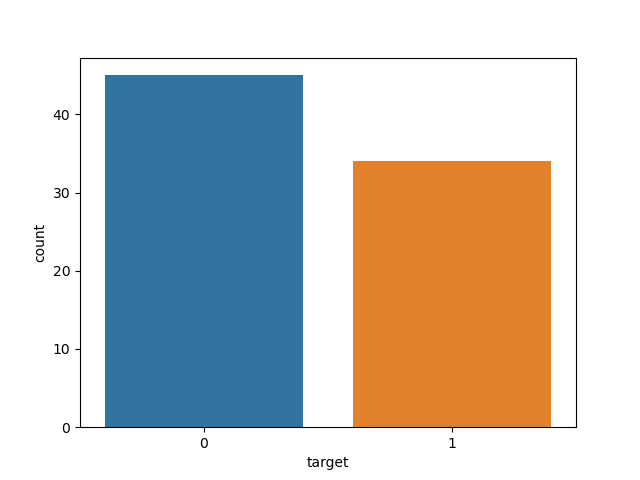
\includegraphics[scale=0.3]{images/kindey_tot.png}
\end{figure}


\begin{figure}[H]
     \centering
     \begin{subfigure}[b]{0.3\textwidth}
         \ \caption{Histograma das variáveis numéricas na população total.}
 \label{fig:var:1:kindney}
 \centering
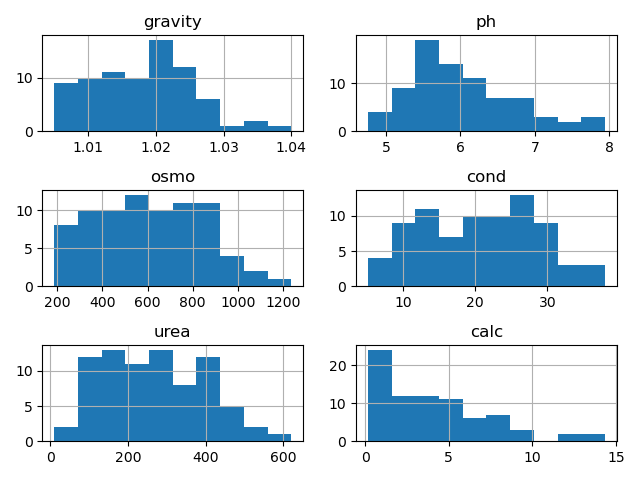
\includegraphics[scale=0.3]{images/hist_kindey_t.png}
     \end{subfigure}
     \hfill
     \begin{subfigure}[b]{0.3\textwidth}
         \centering
         \caption{Histograma das variáveis numéricas na população com Insuficiência Renal.}
 \label{fig:var:2:kindney}
 \centering
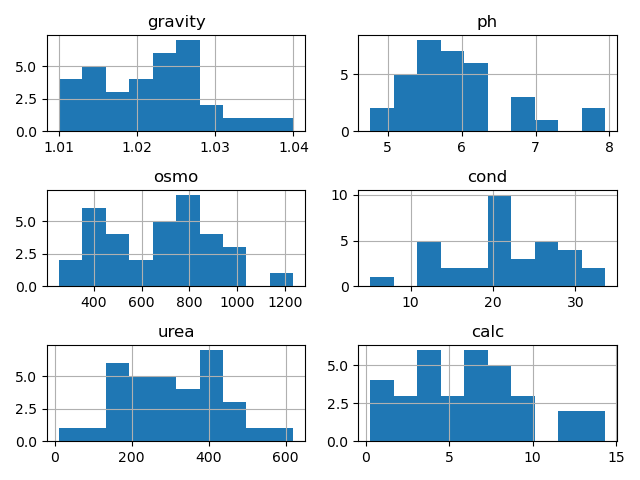
\includegraphics[scale=0.3]{images/hist_kindey_yes.png}
     \end{subfigure}
     \hfill
     \begin{subfigure}[b]{0.3\textwidth}
 \caption{Histograma das variáveis numéricas na população sem Insuficiência Renal.}
 \label{fig:var:3:kindney}
 \centering
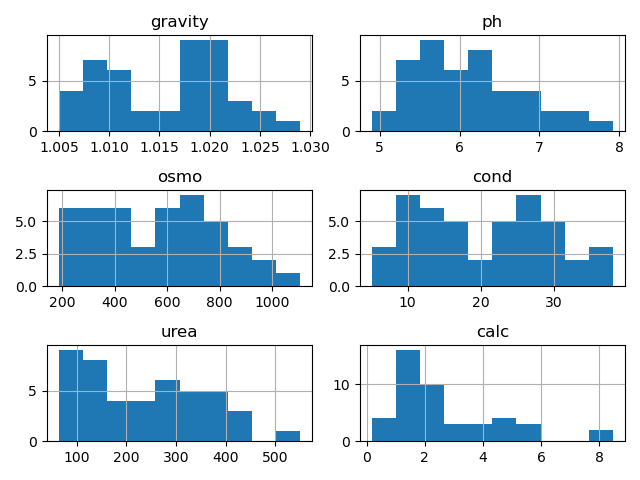
\includegraphics[scale=0.3]{images/hist_kindey_no.png}
     \end{subfigure}
        \caption{Distribuição das variáveis numéricas no conjunto de dados de Insuficiência Renal.}
         \label{fig:var:kindney:t}
\end{figure}

Neste conjunto de dados todos os valores das colunas já são numéricos e não tem \textit{missing}, nenhum tratamento para os dados será necessário. Podendo já utilizar eles na construção dos modelos.
\subsection{Carcinoma da Mama}
O quarto conjunto de dados é o \href{https://www.kaggle.com/datasets/uciml/breast-cancer-wisconsin-data}{Breast Cancer Wisconsin (Diagnostic) Data Set}. Esse conjunto de dados possui características calculadas a partir de uma imagem digitalizada de um aspirado com agulha fina (PAAF) de uma massa mamária. Eles descrevem características dos núcleos celulares presentes na imagem. E o objetivo é diagnosticar o carcinoma da mama como benigno ou maligno.
\begin{itemize}
    \item \textbf{Raio:} média das distâncias do centro aos pontos do perímetro.
    \item \textbf{Textura:} desvio padrão dos valores da escala de cinza.
    \item \textbf{Perímetro:} perímetro calculado para cada núcleo celular
    \item \textbf{Área:} área calculada para cada núcleo celular
    \item \textbf{Suavidade:} variação local nos comprimentos dos raios.
    \item \textbf{Compacidade:} perímetro$^2$ / área - 1,0.
    \item \textbf{Dimensão Fractal:} "aproximação da costa" - 1
    \item \textbf{Simetria:} perímetro$^2$ / área - 1,0.
    \item \textbf{Pontos Côncavos:} número de porções côncavas do contorno.
    \item \textbf{Diagnóstico:} M = maligno, B = benigno.
\end{itemize}

\begin{table}[H]
\label{descritivo:cancer}
\centering
\begin{tabular}{|c|c|c|}
\hline
\textbf{Coluna} & \textbf{dtypes} & \textbf{\textit{NaN}}\\
\hline
id                         &  int64 & 0 \\
\hline
diagnosis                  & object & 0 \\
\hline
radius\_mean               & float64 & 0 \\
\hline
texture\_mean             &  float64 & 0 \\
\hline
perimeter\_mean           &  float64 & 0 \\
\hline
area\_mean               &   float64 & 0 \\
\hline
smoothness\_mean          &  float64 & 0 \\
\hline
compactness\_mean         &  float64 & 0 \\
\hline
concavity\_mean          &   float64 & 0 \\
\hline
concave points\_mean      &  float64 & 0 \\
\hline
symmetry\_mean            &  float64 & 0 \\
\hline
fractal\_dimension\_mean   &  float64 & 0 \\
\hline
radius\_se                &  float64 & 0 \\
\hline
texture\_se              &   float64 & 0 \\
\hline
perimeter\_se            &   float64 & 0 \\
\hline
area\_se                 &   float64 & 0 \\
\hline
smoothness\_se           &   float64 & 0 \\
\hline
compactness\_se          &   float64 & 0 \\
\hline
concavity\_se            &   float64 & 0 \\
\hline
concave points\_se       &   float64 & 0 \\
\hline
symmetry\_se             &   float64 & 0 \\
\hline
fractal\_dimension\_se   &    float64 & 0 \\
\hline
radius\_worst           &    float64 & 0 \\
\hline
texture\_worst         &     float64 & 0 \\
\hline
perimeter\_worst       &     float64 & 0 \\
\hline
area\_worst            &     float64 & 0 \\
\hline
smoothness\_worst      &     float64 & 0 \\
\hline
compactness\_worst     &     float64 & 0 \\
\hline
concavity\_worst       &     float64 & 0 \\
\hline
concave points\_worst  &     float64 & 0 \\
\hline
symmetry\_worst        &     float64 & 0 \\
\hline
fractal\_dimension\_worst   & float64 & 0 \\
\hline
\end{tabular}
\caption{Tabela com o tipo de cada variável e quantidade de linhas \textit{NaN} em cada coluna no conjunto de dados de Carcinoma da Mama.}
\end{table}
\begin{figure}[H]
 \centering
        \caption{Estatística descritiva das variáveis numéricas no conjunto de dados de Carcinoma da Mama.}
         \label{fig:var:cancer:desc}
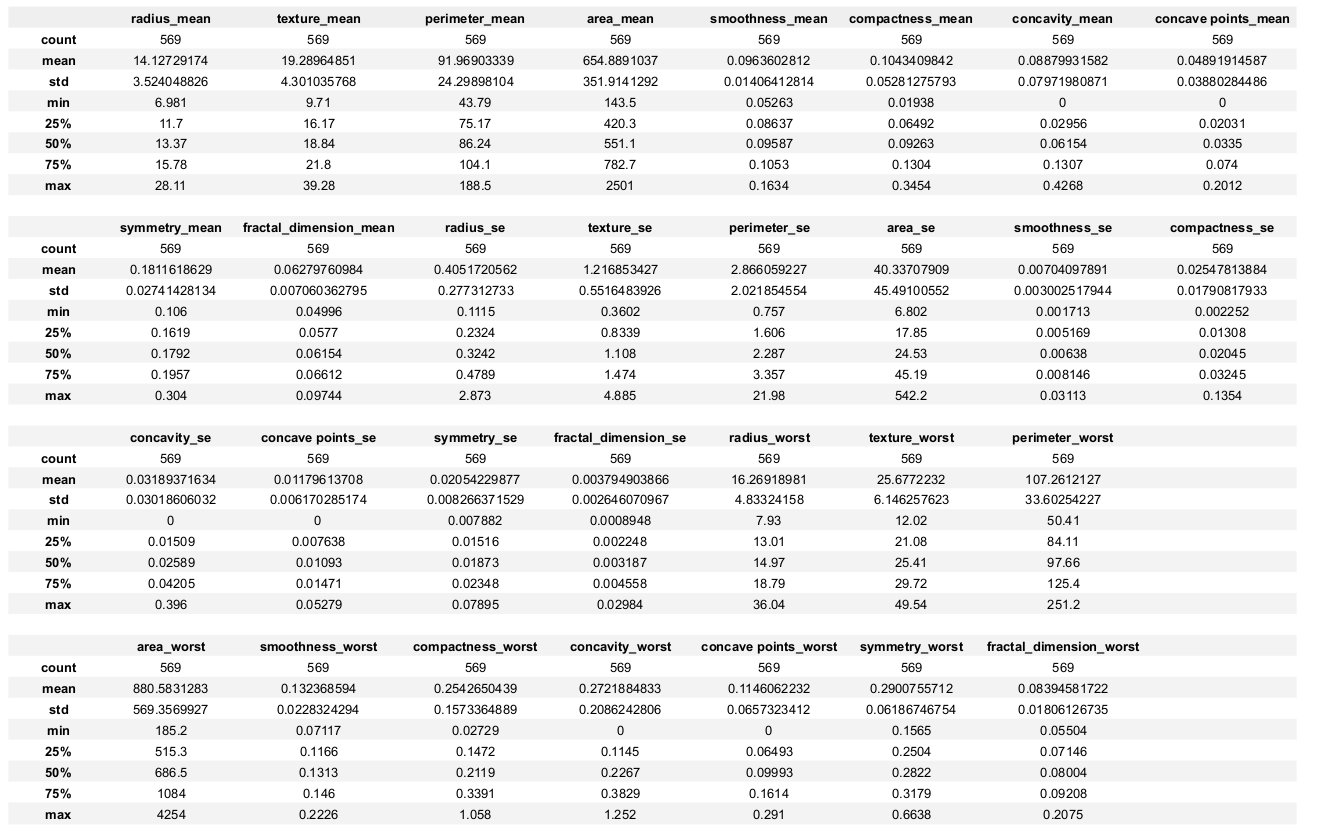
\includegraphics[scale=0.3]{images/descritiva_cancer.png}
\end{figure}
\begin{figure}[H]
 \centering
        \caption{Distribuição de Carcinoma da Mama Maligno e Benigno na população.}
         \label{fig:var:cancer:tot:pop}
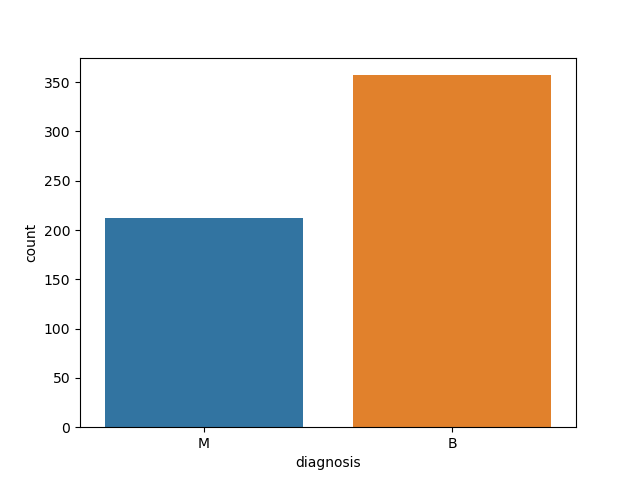
\includegraphics[scale=0.3]{images/cancertot.png}
\end{figure}

\begin{figure}[H]
     \centering
     \begin{subfigure}[b]{0.3\textwidth}
 \centering
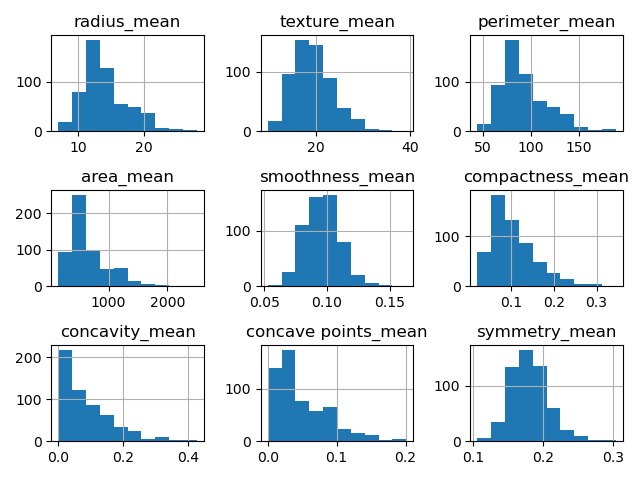
\includegraphics[scale=0.3]{images/hist_cancer_t.png}
     \end{subfigure}
     \hfill
     \begin{subfigure}[b]{0.3\textwidth}
         \centering
 \centering
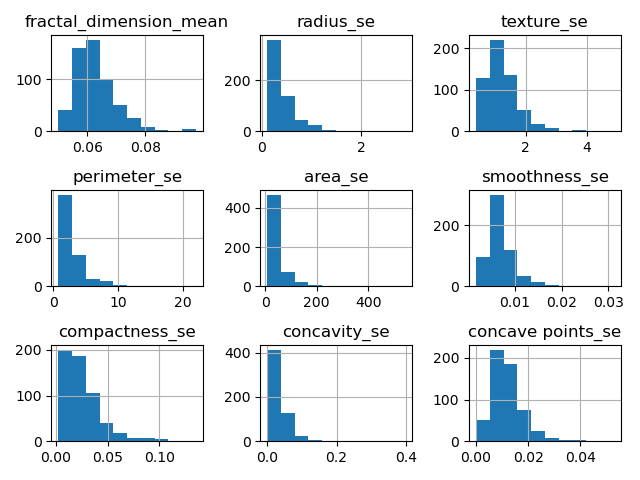
\includegraphics[scale=0.3]{images/hist_cancer_t_2.png}
     \end{subfigure}
     \hfill
     \begin{subfigure}[b]{0.3\textwidth}
 \centering
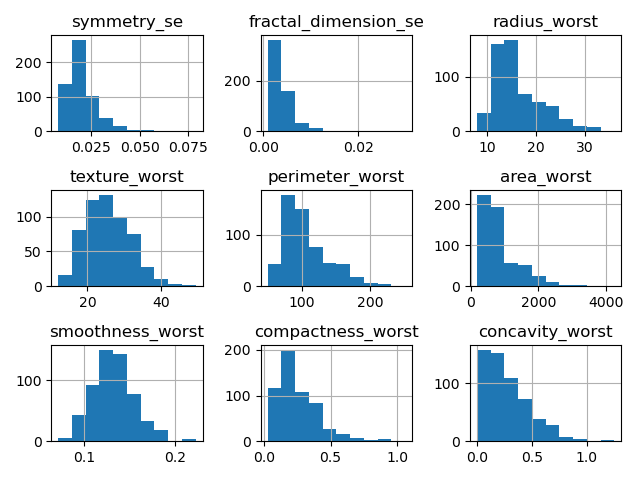
\includegraphics[scale=0.3]{images/hist_cancer_t_3.png}
     \end{subfigure}
          \hfill
     \begin{subfigure}[b]{0.3\textwidth}
 \centering
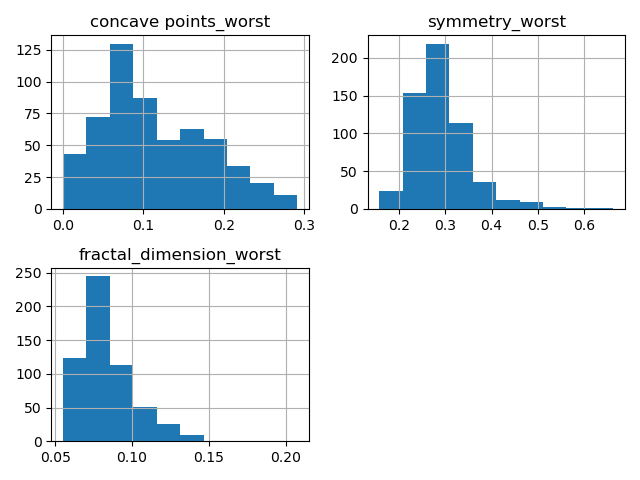
\includegraphics[scale=0.3]{images/hist_cancer_t_4.png}
     \end{subfigure}
        \caption{Distribuição das variáveis numéricas no conjunto de dados de Carcinoma da Mama.}
         \label{fig:var:cancer:t}
\end{figure}

\begin{figure}[H]
     \centering
     \begin{subfigure}[b]{0.3\textwidth}
 \centering
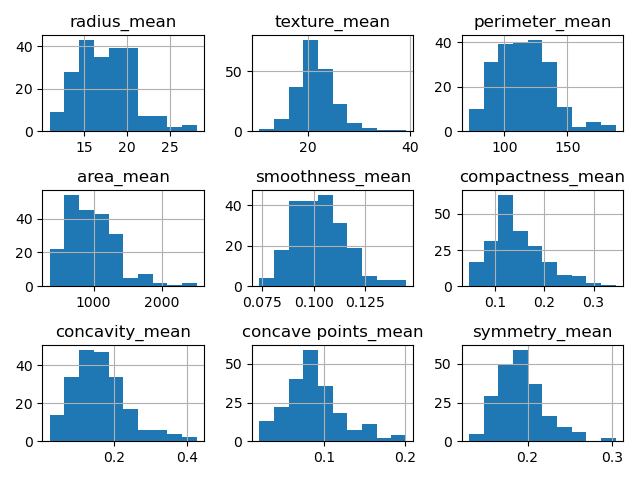
\includegraphics[scale=0.3]{images/hist_cancer_yes_1.png}
     \end{subfigure}
     \hfill
     \begin{subfigure}[b]{0.3\textwidth}
         \centering
 \centering
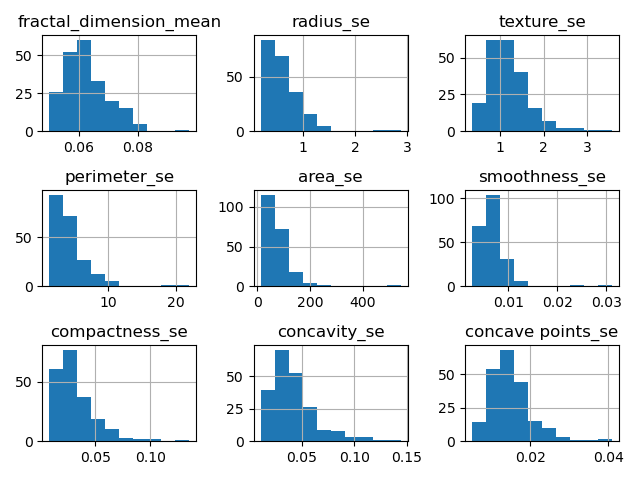
\includegraphics[scale=0.3]{images/hist_cancer_yes_2.png}
     \end{subfigure}
     \hfill
     \begin{subfigure}[b]{0.3\textwidth}
 \centering
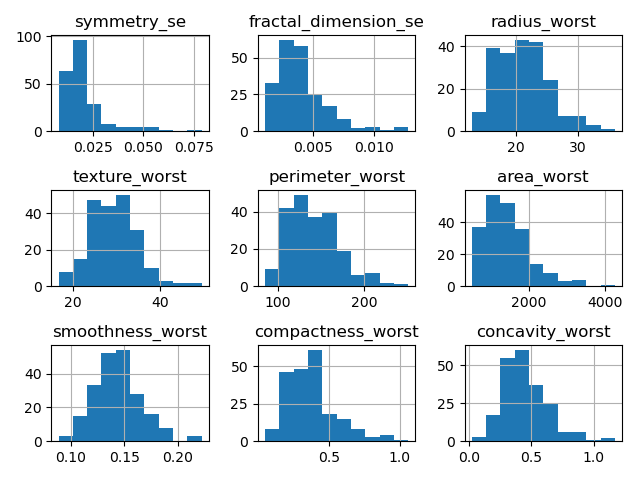
\includegraphics[scale=0.3]{images/hist_cancer_yes_3.png}
     \end{subfigure}
          \hfill
     \begin{subfigure}[b]{0.3\textwidth}
 \centering
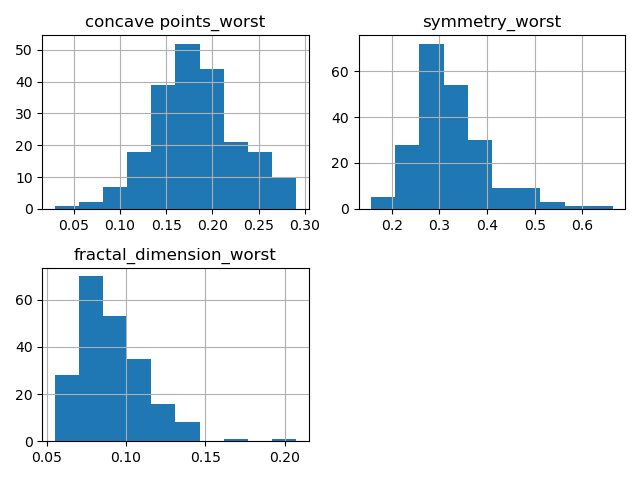
\includegraphics[scale=0.3]{images/hist_cancer_yes_4.png}
     \end{subfigure}
        \caption{Distribuição das variáveis numéricas no conjunto de dados da população com Carcinoma da Mama Maligno.}
         \label{fig:var:cancer:m}
\end{figure}

\begin{figure}[H]
     \centering
     \begin{subfigure}[b]{0.3\textwidth}
 \centering
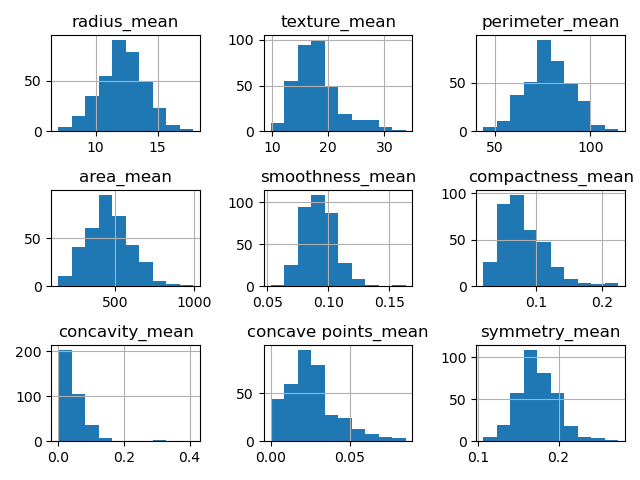
\includegraphics[scale=0.3]{images/hist_cancer_no_1.png}
     \end{subfigure}
     \hfill
     \begin{subfigure}[b]{0.3\textwidth}
         \centering
 \centering
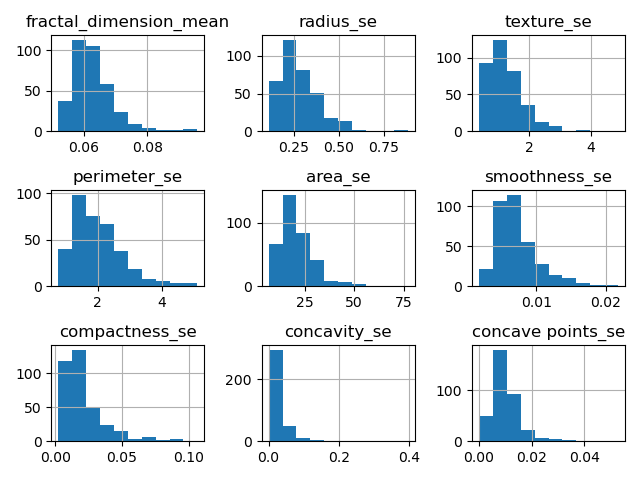
\includegraphics[scale=0.3]{images/hist_cancer_no_2.png}
     \end{subfigure}
     \hfill
     \begin{subfigure}[b]{0.3\textwidth}
 \centering
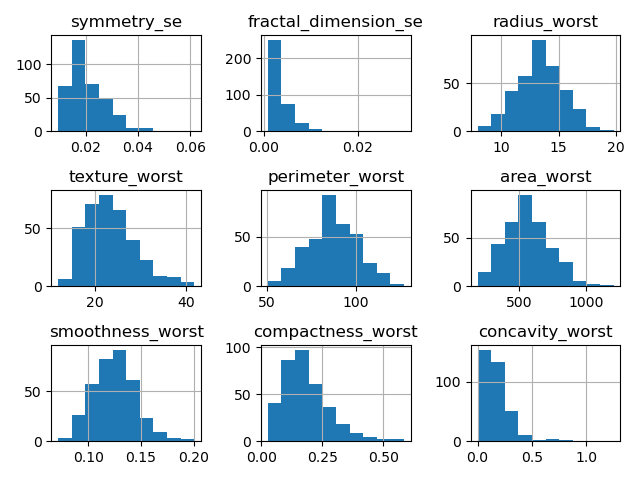
\includegraphics[scale=0.3]{images/hist_cancer_no_3.png}
     \end{subfigure}
          \hfill
     \begin{subfigure}[b]{0.3\textwidth}
 \centering
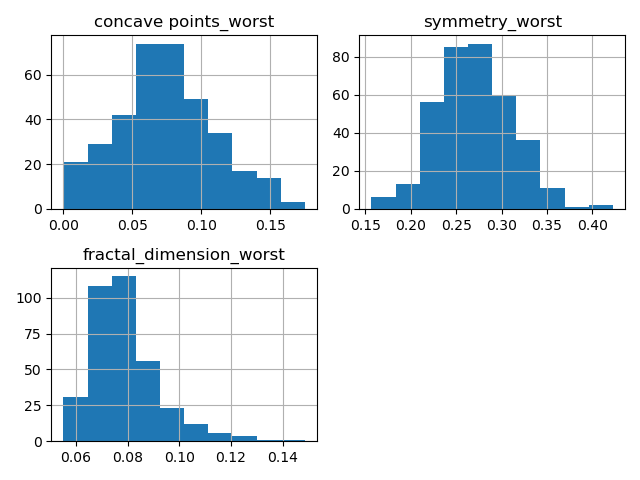
\includegraphics[scale=0.3]{images/hist_cancer_no_4.png}
     \end{subfigure}
        \caption{Distribuição das variáveis numéricas no conjunto de dados da população com Carcinoma da Mama Benigno.}
         \label{fig:var:cancer:b}
\end{figure}


Neste conjunto de dados é necessário criar a variável target 0 ou 1 a partir da coluna
\textbf{diagnosis} e a remoção da coluna \textbf{Unnamed: 32} do conjunto de dados. Após isso os dados já podem ser utilizados para o treino dos modelos preditivos.

\section{Métricas de Validação de Performance e Desempenho}
Para as métricas de performance, utilizamos a AUC, logloss e o KS. O código CITAR mostra a implementação em python dessas métricas.
\begin{codigo}[caption={Código implementado o cálculo da AUC, logloss e o KS.}, label={codigo:im:auc:ks:log}, language=Python, breaklines=true]
def auc_logloss_ks(y_test, y_prob):
    '''
    Input:
        y_prob: model predict prob
        y_test: target
    Output: Metrics of validation
        auc, ks, log_loss
    '''
    fpr, tpr, thresholds = metrics.roc_curve(y_test, y_prob)
    auc = metrics.auc(fpr, tpr)
    log_loss = sklearn.metrics.log_loss(y_test, y_prob)
    ks = max(tpr - fpr)
    return auc, log_loss, ks
\end{codigo}

Para o custo computacional, utilizou-se a biblioteca \textbf{timeit} para o cálculo em nanosegundos. Basta iniciar antes do treino de cada modelo e no final teremos o tempo calculado. O código \ref{codigo:ex:timeit} exemplifica o processo.
\begin{codigo}[caption={Importação da biblioteca timeit e o cálculo em segundos da execução do código.}, label={codigo:ex:timeit}, language=Python, breaklines=true]
import timeit
start = timeit.default_timer()
model_XGB = train(X_train, y_train, X_test, y_test, balanced='balanced', method='XGBoost', number_trials=100)
stop = timeit.default_timer()
stop - start
\end{codigo}

\section{Divisão de Treino e Teste}
Iremos utilizar a função \textit{train\_test\_split} do \textbf{sklearn} para separar o nosso conjunto de treino e teste. $\text{X}$ representa as variáveis explicativas que entraram no treino do modelo e o $y$ representa a variável resposta, target. Não será utilizado o conjunto de validação, pois temos pouco volume de dados em alguns conjunto de dados.

Para os conjunto de dados que possuem apenas dados numéricos será utilizado o mesmo conjunto de treino e teste para todos os modelos, enquanto que os conjunto de dados que possuem variáveis categóricas serão divididos em um conjunto de dados só numéricos para o XGBoost e LightGBM e outro conjunto com variáveis numéricas e categóricas para o CatBoost.
\begin{codigo}[caption={Exemplo da divisão dos conjuntos de treino e teste.}, label={codigo:ex:trainteste_split}, language=Python, breaklines=true]
X_train, X_test, y_train, y_test = train_test_split(X, y, test_size=0.3, random_state=42)
\end{codigo}

\section{Espaço de Hiperparâmetros}
Conforme abordado em \ref{cap3:hiper}, temos alguns parâmetros que são comuns para os três algoritmos, nesta primeira parte do estudo em que vamos alterar os hiperparâmetros manualmente vamos focar neles: \textbf{learning\_rate , max\_depth, n\_estimators, reg\_lambda}. Vamos denotar os hiperparâmetros respectivamente como $LR$, \simbolo{MD}{max\_depth, hiperparâmetro da profundidade máxima}$MD$, \simbolo{RegL}{reg\_lambda, hiperparâmetro da regularização $L_2$}$RegL$. E os valores que vamos testar são:

\begin{gather*}
    LR = \{0.1,0.3\}\\
    MD = \{3,6\}\\
    RegL = \{0.01,0.05\}
\end{gather*}
\section{Tuning do modelo com o Optuna}
Para o tuning com o Optuna foi criada a função objetivo, tuning e o train, de forma que a existência de variáveis categóricas no conjunto de dados já é identificada e, para o caso do \textit{CatBoost}, as separada automaticamente.

O código \ref{codigo:im:tuning} mostra todos os parâmetros das funções e o espaço dos hiperparâmetros que o Optuna irá percorrer para realizar o processo de tuning em cada um dos algoritmos diferentes. Foi utilizado 1 hora como o tempo máximo para o Optuna tunar cada algoritmo, ou seja, cada conjunto de dados demorou cerca de 3 horas para obter os resultados finais.

\begin{codigo}[caption={Código implementado para o Tuning com o Optuna.}, label={codigo:im:tuning}, language=Python, breaklines=true]
import numpy as np
import pandas as pd
import xgboost as xgb
import sys
import timeit
import gc
import sklearn
import seaborn

from sklearn import metrics
from xgboost import XGBClassifier
from catboost import CatBoostClassifier
from sklearn.model_selection import train_test_split
import lightgbm
from lightgbm import LGBMClassifier
from sklearn.metrics import roc_auc_score
from sklearn.metrics import accuracy_score
import optuna
from sklearn.model_selection import GridSearchCV
import matplotlib.pylab as plt
from sklearn.model_selection import cross_val_score
from sklearn.model_selection import StratifiedKFold
from optuna.visualization import plot_optimization_history
from optuna.visualization import plot_param_importances

def auc_logloss_ks(y_test, y_prob):
    '''
    Input:
        y_prob: model predict prob
        y_test: target
    Output: Metrics of validation
        auc, ks, log_loss
    '''
    fpr, tpr, thresholds = metrics.roc_curve(y_test, y_prob)
    auc = metrics.auc(fpr, tpr)
    log_loss = sklearn.metrics.log_loss(y_test, y_prob)
    ks = max(tpr - fpr)
    return auc, log_loss, ks

def objective(trial, X_train, y_train, X_test, y_test, balanced, method):
    '''
    Input:
        trial: trial of the test
        X_train:
        y_train:
        X_test:
        y_test:
        balanced:balanced or None
        method: XGBoost, CatBoost or LGBM
    Output: Metrics of validation
        auc, ks, log_loss
        auc_logloss_ks(y_test, y_pred)[0]
    '''
    gc.collect()
    if method=='LGBM':
        param_grid = {'learning_rate': trial.suggest_float('learning_rate', 0.0001, 0.1, log=True),
                      'num_leaves': trial.suggest_int('num_leaves', 2, 256),
                      'lambda_l1': trial.suggest_float("lambda_l1", 1e-8, 10.0, log=True),
                      'lambda_l2': trial.suggest_float("lambda_l2", 1e-8, 10.0, log=True),
                      'min_data_in_leaf': trial.suggest_int('min_data_in_leaf', 5, 100),
                      'max_depth': trial.suggest_int('max_depth', 5, 64),
                      'feature_fraction': trial.suggest_float("feature_fraction", 0.4, 1.0),
                      'bagging_fraction': trial.suggest_float("bagging_fraction", 0.4, 1.0),
                      'bagging_freq': trial.suggest_int("bagging_freq", 1, 7),
  
                     }
        model = LGBMClassifier(**param_grid)

        print('LGBM - Optimization using optuna')
        model.fit(X_train, y_train)
        
        y_pred = model.predict_proba(X_test)[:,1]

    if method=='CATBoost':
        param_grid = {'learning_rate': trial.suggest_float('learning_rate', 0.0001, 0.1, log=True),
                      'depth': trial.suggest_int("depth", 4, 10),
                      'max_bin': trial.suggest_int('max_bin', 200, 400),
                      'min_data_in_leaf': trial.suggest_int('min_data_in_leaf', 1, 300),
                      'l2_leaf_reg': trial.suggest_float('l2_leaf_reg', 1e-8, 10, log = True),
                      'random_seed': 42,
                      'random_strength': trial.suggest_float("random_strength", 1e-8, 10.0, log=True),
                      'bagging_temperature': trial.suggest_float("bagging_temperature", 0.0, 10.0),
                      'od_type': trial.suggest_categorical("od_type", ["IncToDec", "Iter"]),
                      'od_wait': trial.suggest_int("od_wait", 10, 50),
                     }
        if len(X_train._get_numeric_data().columns) != len(X_train.columns):
            categorical_features_indices = list(X_train.select_dtypes(exclude='number').columns)
            model = CatBoostClassifier(**param_grid)
            print('CATBoost - Optimization using optuna')
            model.fit(X_train, y_train,cat_features=categorical_features_indices,verbose=False)
            y_pred = model.predict_proba(X_test)[:,1]
        else:
            model = CatBoostClassifier(**param_grid)
            print('CATBoost - Optimization using optuna')
            model.fit(X_train, y_train,verbose=False)
            y_pred = model.predict_proba(X_test)[:,1]
        
    if method=='XGBoost':
        param_grid = {'learning_rate': trial.suggest_float('learning_rate', 0.0001, 0.1, log=True),
                      'max_depth': trial.suggest_int('max_depth', 3, 16),
                      'min_child_weight': trial.suggest_int('min_child_weight', 1, 300),
                      'gamma': trial.suggest_float('gamma', 1e-8, 1.0, log = True),
                      'alpha': trial.suggest_float('alpha', 1e-8, 1.0, log = True),
                      'lambda': trial.suggest_float('lambda', 0.0001, 10.0, log = True),
                      'colsample_bytree': trial.suggest_float('colsample_bytree', 0.1, 0.8),
                      'booster': 'gbtree',
                      'random_state': 42,
                     }
        model = XGBClassifier(**param_grid)
        print('XGBoost - Optimization using optuna')
        model.fit(X_train, y_train,verbose=False)
        y_pred = model.predict_proba(X_test)[:,1]
    
    auc_res, log_loss_res, ks_res = auc_logloss_ks(y_test, y_pred)
    print('auc:'+str(auc_res),', log_loss:'+str(log_loss_res),', ks:'+str(ks_res))
    return auc_logloss_ks(y_test, y_pred)[0]

def tuning(X_train, y_train, X_test, y_test, balanced, method):
    '''
    Input:
        trial: 
        x_train:
        y_train:
        X_test:
        y_test:
        balanced:balanced or not balanced
        method: XGBoost, CatBoost or LGBM
    Output: Metrics of validation
        auc, ks, log_loss
        auc_logloss_ks(y_test, y_pred)[0]
    '''
    study = optuna.create_study(direction='maximize', study_name=method+' Classifier')
    func = lambda trial: objective(trial, X_train, y_train, X_test, y_test, balanced, method)
    print('Starting the optimization')
    time_max_tuning = 60*30 # max time in seconds to stop
    study.optimize(func, timeout=time_max_tuning)
    return study

def train(X_train, y_train, X_test, y_test, balanced, method):
    '''
    Input:
        X_train:
        y_train:
        X_test:
        y_test:
        balanced:balanced or None
        method: XGBoost, CatBoost or LGBM
    Output: predict model
    '''
    print('Tuning')
    study = tuning(X_train, y_train, X_test, y_test, balanced, method)
    if method=='LGBM':
        model = LGBMClassifier(**study.best_params)
        print('Last Fit')
        model.fit(X_train, y_train, eval_set=[(X_test,y_test)],
                 callbacks = [lightgbm.early_stopping(stopping_rounds=100), lightgbm.log_evaluation(period=5000)])
    if method=='CATBoost':
        model = CatBoostClassifier(**study.best_params)
        if len(X_train._get_numeric_data().columns) != len(X_train.columns):
            categorical_features_indices = list(X_train.select_dtypes(exclude='number').columns)
            print('Last Fit')
            model.fit(X_train, y_train,cat_features=categorical_features_indices, eval_set=[(X_test,y_test)],
                 early_stopping_rounds=100,verbose = False)
        else:
            print('Last Fit')
            model.fit(X_train, y_train, eval_set=[(X_test,y_test)],
                 early_stopping_rounds=100,verbose = False)
    if method=='XGBoost':
        model = XGBClassifier(**study.best_params)
        print('Last Fit')
        model.fit(X_train, y_train, eval_set=[(X_test,y_test)],
                 early_stopping_rounds=100,verbose = False)
    return model, study
\end{codigo}

\section{Explicabilidade dos Modelos}
Para as versões finais de cada modelo, que são aquelas que obtiveram as melhores métricas de performance, iremos aplicar os Valores de SHAP para realizar a explicabilidade de cada variável e seu impacto no modelo final.

O código \ref{codigo:ex:shap} demonstra como é a execução do SHAP.
\begin{codigo}[caption={Importação da biblioteca shap e o cálculo dos shap values.}, label={codigo:ex:shap}, language=Python, breaklines=true]
import shap
explainer = shap.TreeExplainer(model_XGB)
shap_values = explainer.shap_values(X_train)
shap.summary_plot(shap_values, X_train,plot_size=.7)
\end{codigo}






\chapter{Análise Experimental}
\label{chapter:experimental}
\label{cap:exper}
Nesta seção serão mostrados os resultados experimentais do capítulo \ref{cap:desen}. As saídas de alguns resultados podem ser encontradas no arquivo Jupyter-notebook no \href{https://github.com/joaomh/study_boosting_optuna_USP_undergraduate_thesis}{GitHub}. As análises consistem em alterar os hiperparâmetros, conforme explicado no capítulo \ref{cap:desen}, depois aplicar o Optuna para os 3 modelos, com o tempo máximo de execução de trinta minutos para cada um.
\section{Resultados de Conjunto de dados de Diabetes}
\begin{table}[H]
\centering
\begin{tabular}{|c|c|c|c|}
\hline
	& \textbf{XGBoost} &\textbf{CatBoost} & \textbf{LightGBM} \\
\hline
\textbf{AUC}	&0.93639	& 0.89655	& 0.92066 \\
\hline
\textbf{logloss}	& 1.69072 & 2.65684	& 2.29456 \\
\hline
\textbf{KS}	& 0.87278	& 0.79311	& 0.84131 \\
\hline
\textbf{tempo (s)}	& 0.17799 &	 1.78698 &	0.08261 \\
\hline
\end{tabular}
\caption{Resultado do XGBoost, CatBoost e LGBM com os hiperparâmetros \textit{Default} no conjunto de dados de diabetes.}\label{res:dia:1}
\end{table}

\begin{table}[H]
\label{res:dia:2}
\centering
\begin{tabular}{|c|c|c|c|}
\hline
	& \textbf{XGBoost} &\textbf{CatBoost} & \textbf{LightGBM} \\
\hline
\textbf{AUC}	& 0.92598	& 0.89428	& 0.89406\\
\hline
\textbf{logloss}	& 2.17379	& 3.13992	& 2.89838\\
\hline
\textbf{KS}	& 0.85195	& 0.78856	0& 0.78812 \\
\hline
\textbf{tempo (s)}	& 0.10825	& 1.05492	& 0.09304 \\
\hline
\end{tabular}
\caption{Resultado do XGBoost, CatBoost e LGBM com os hiperparâmetros $LR=0.1$, $MD=3$, $Reg_L=0.01$ no conjunto de dados de diabetes.}
\end{table}

\begin{table}[H]
\label{res:dia:3}
\centering
\begin{tabular}{|c|c|c|c|}
\hline
	& \textbf{XGBoost} &\textbf{CatBoost} & \textbf{LightGBM} \\
\hline
\textbf{AUC}	& 0.92598	&0.90448	&0.92598\\
\hline
\textbf{logloss}	& 2.17379	&2.41531	&2.17379\\
\hline
\textbf{KS}	& 0.85195	& 0.80895 &	0.85195 \\
\hline
\textbf{tempo (s)}	& 0.11743&	1.00966&	0.08180 \\
\hline
\end{tabular}
\caption{Resultado do XGBoost, CatBoost e LGBM com os hiperparâmetros $LR=0.3$, $MD=3$, $Reg_L=0.01$ no conjunto de dados de diabetes.}
\end{table}

\begin{table}[H]
\label{res:dia:4}
\centering
\begin{tabular}{|c|c|c|c|}
\hline
	& \textbf{XGBoost} &\textbf{CatBoost} & \textbf{LightGBM} \\
\hline
\textbf{AUC}	& 0.93107&	0.91534	&0.92066\\
\hline
\textbf{logloss}	& 1.81149	&2.41532	&2.29456\\
\hline
\textbf{KS}	& 0.86215	& 0.83067	& 0.84131\\
\hline
\textbf{tempo (s)}	& 0.12579	&1.82060	&0.11067\\
\hline
\end{tabular}
\caption{Resultado do XGBoost, CatBoost e LGBM com os hiperparâmetros $LR=0.1$, $MD=6$, $Reg_L=0.01$ no conjunto de dados de diabetes.}
\end{table}

\begin{table}[H]
\label{res:dia:5}
\centering
\begin{tabular}{|c|c|c|c|}
\hline
	& \textbf{XGBoost} &\textbf{CatBoost} & \textbf{LightGBM} \\
\hline
\textbf{AUC}	& 0.89406	&0.89428	&0.89406\\
\hline
\textbf{logloss}	& 2.89838	&3.13992&	2.89838\\
\hline
\textbf{KS}	& 0.78812&	0.78856 &	0.78812\\
\hline
\textbf{tempo (s)}	& 0.09512	&1.38364	&0.08838\\
\hline
\end{tabular}
\caption{Resultado do XGBoost, CatBoost e LGBM com os hiperparâmetros $LR=0.1$, $MD=3$, $Reg_L=0.05$ no conjunto de dados de diabetes.}
\end{table}

\begin{table}[H]
\label{res:dia:6}
\centering
\begin{tabular}{|c|c|c|c|}
\hline
	& \textbf{XGBoost} &\textbf{CatBoost} & \textbf{LightGBM} \\
\hline
\textbf{AUC}	& 0.93107&	0.89927	&0.92598\\
\hline
\textbf{logloss}	& 1.81149	&2.65685	&2.17379\\
\hline
\textbf{KS}	& 0.86215	&0.79854	&0.85195 \\
\hline
\textbf{tempo (s)}	& 0.13494	&2.58085	&0.09262 \\
\hline
\end{tabular}
\caption{Resultado do XGBoost, CatBoost e LGBM com os hiperparâmetros $LR=0.3$, $MD=6$, $Reg_L=0.01$ no conjunto de dados de diabetes.}
\end{table}

\begin{table}[H]
\label{res:dia:7}
\centering
\begin{tabular}{|c|c|c|c|}
\hline
	& \textbf{XGBoost} &\textbf{CatBoost} & \textbf{LightGBM} \\
\hline
\textbf{AUC}	& 0.92836	&0.90470	&0.92598\\
\hline
\textbf{logloss}	& 1.81148&	2.65685&	2.17379\\
\hline
\textbf{KS}	&0.85672&	0.80940	&0.85195\\
\hline
\textbf{tempo (s)}	& 0.13301	&1.81456	&0.10295 \\
\hline
\end{tabular}
\caption{Resultado do XGBoost, CatBoost e LGBM com os hiperparâmetros $LR=0.3$, $MD=6$, $Reg_L=0.05$ no conjunto de dados de diabetes.}
\end{table}

\begin{table}[H]
\label{res:dia:8}
\centering
\begin{tabular}{|c|c|c|c|}
\hline
	& \textbf{XGBoost} &\textbf{CatBoost} & \textbf{LightGBM} \\
\hline
\textbf{AUC}	& 0.92598&	0.90492&	0.92598\\
\hline
\textbf{logloss}	& 2.17379&	2.89839	&2.17379\\
\hline
\textbf{KS}	& 0.85195	&0.80984	&0.85195 \\
\hline
\textbf{tempo (s)}	& 0.10512&	0.97739	&0.09690 \\
\hline
\end{tabular}
\caption{Resultado do XGBoost, CatBoost e LGBM com os hiperparâmetros $LR=0.3$, $MD=3$, $Reg_L=0.05$ no conjunto de dados de diabetes.}
\end{table}
\subsection{Optuna no Conjunto de dados de Diabetes}
No final da execução, o Optuna nos retorna a quantidade de \textit{trials} e qual foi a que obteve a melhor performance. Abaixo temos os códigos com as melhores saídas do Optuna de cada modelo.
\begin{codigo}[caption={Resultado do Optuna no conjunto de dados de Diabetes.}, label={codigo:res:op:dia}, language=Python, breaklines=true]
XGBoost_model = train(X_train, y_train, X_test, y_test, balanced='balanced', method='XGBoost')
Trial 5143 finished with value: 0.9734596631205674 and parameters: {'learning_rate': 0.08503540937695053, 'max_depth': 16, 'min_child_weight': 1, 'gamma': 0.3765138366132899, 'alpha': 0.00011157064804299481, 'lambda': 0.06609519167136822, 'colsample_bytree': 0.7351361006258642}. Best is trial 5052 with value: 0.9759530141843972.
...
Trial 5052 finished with value: 0.9759530141843972 and parameters: {'learning_rate': 0.09999081729983263, 'max_depth': 15, 'min_child_weight': 1, 'gamma': 0.7591251036860868, 'alpha': 0.00010662969781278809, 'lambda': 0.06239587908284276, 'colsample_bytree': 0.7655930247173538}. Best is trial 5052 with value: 0.9759530141843972.
XGBoost - Optimization using optuna
auc:0.9759530141843972 , log_loss:0.17300349809156104 , ks:0.8782136524822696

CatBoost_model = train(X_train_cat, y_train_cat, X_test_cat, y_test_cat, balanced='balanced', method='CATBoost')
Trial 230 finished with value: 0.9786125886524822 and parameters: {'learning_rate': 0.008066790947749524, 'depth': 10, 'max_bin': 282, 'min_data_in_leaf': 48, 'l2_leaf_reg': 2.120609777416555, 'random_strength': 1.9674219542672667e-06, 'bagging_temperature': 6.752333264637867, 'od_type': 'Iter', 'od_wait': 16}. Best is trial 160 with value: 0.9811059397163121.
...
Trial 160 finished with value: 0.9811059397163121 and parameters: {'learning_rate': 0.005585552379158199, 'depth': 10, 'max_bin': 316, 'min_data_in_leaf': 11, 'l2_leaf_reg': 1.1081451827078879, 'random_strength': 7.466692400471057e-07, 'bagging_temperature': 9.443675875030443, 'od_type': 'IncToDec', 'od_wait': 17}. Best is trial 160 with value: 0.9811059397163121.
CATBoost - Optimization using optuna
auc:0.9811059397163121 , log_loss:0.17088682855569354 , ks:0.8779920212765957

LGBM_model = train(X_train, y_train, X_test, y_test, balanced='balanced', method='LGBM')
Trial 4540 finished with value: 0.9765625 and parameters: {'learning_rate': 0.07003556517783399, 'num_leaves': 191, 'lambda_l1': 3.2225284078443206e-06, 'lambda_l2': 4.1456610637867624e-08, 'min_data_in_leaf': 11, 'max_depth': 55, 'feature_fraction': 0.9234036984685567, 'bagging_fraction': 0.630684594822488, 'bagging_freq': 6}. Best is trial 1283 with value: 0.9816626773049646.
...
Trial 1283 finished with value: 0.9806626773049646 and parameters: {'learning_rate': 0.08425779644832665, 'num_leaves': 205, 'lambda_l1': 2.7481689793447196e-06, 'lambda_l2': 4.307867154100011e-08, 'min_data_in_leaf': 9, 'max_depth': 63, 'feature_fraction': 0.9232766751662997, 'bagging_fraction': 0.9517850099076617, 'bagging_freq': 6}. Best is trial 1283 with value: 0.9806626773049646.
LGBM - Optimization using optuna
auc:0.9816626773049646 , log_loss:0.1859868135509998 , ks:0.8832003546099291

\end{codigo}

\begin{table}[H]
\centering
\begin{tabular}{|c|c|c|c|}
\hline
	& \textbf{XGBoost} &\textbf{CatBoost} & \textbf{LightGBM} \\
\hline
\textbf{AUC}	& 0.97595	&0.981106	&0.98166\\
\hline
\textbf{logloss}	& 0.17300&	0.17327	&0.18599\\
\hline
\textbf{KS}	& 0.87821&	0.87799&	0.88320\\
\hline
\end{tabular}
\caption{Resultado do XGBoost, CatBoost e LGBM com os hiperparâmetros otimizados pelo Optuna no conjunto de dados de diabetes.}\label{res:dia:op}
\end{table}


\subsection{Resultados do estudo do Optuna no conjunto de dados de Diabetes utilizando o XGBoost.}
A primeira coisa é analisar todos os treinos e os valores encontrados para cada interação do Optuna para cada modelo.
\begin{figure}[H]
 \caption{Valores do estudo do XGBoost no conjunto de dados de Diabetes pelo Optuna.}
 \label{fig:op:dia:trials:xgb}
 \centering
 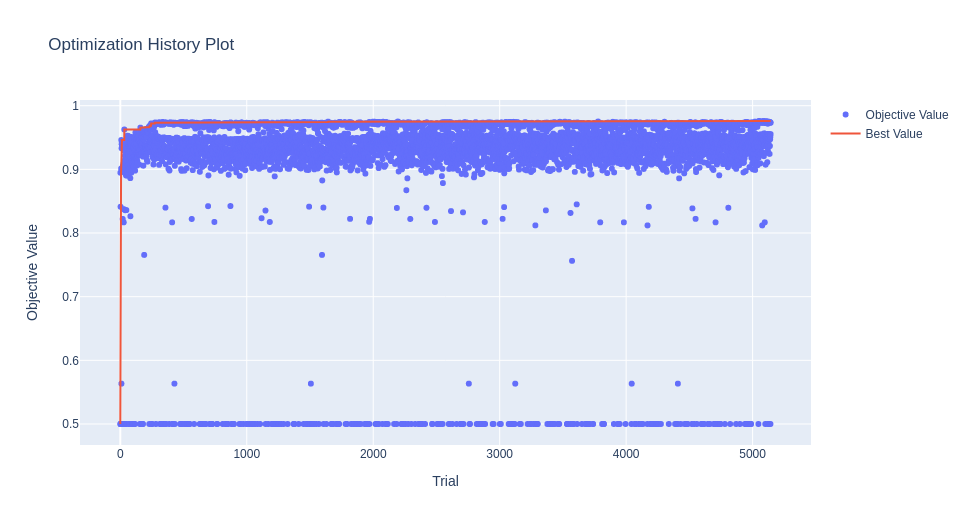
\includegraphics[scale=0.4]{images/optuna_xgboost_dia.png}
\end{figure}
A partir do estudo de otimização do Optuna foi possível identificar quais os hiperparâmetros que possuem o maior impacto no tuning do Optuna.
\begin{figure}[H]
 \caption{Hiperparâmetros do XGBoost com maior importância no Optuna no dados de Diabetes.}
 \label{fig:op:dia:impo:xgb}
 \centering
 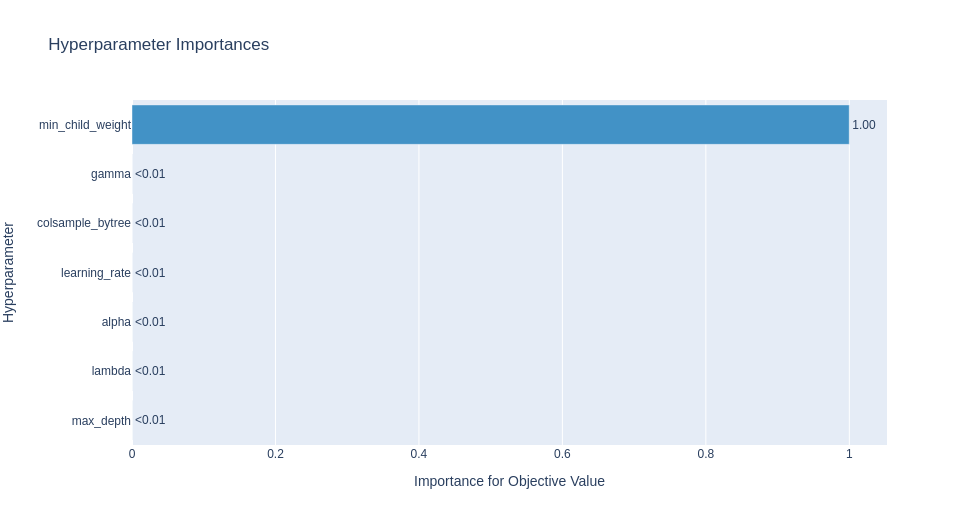
\includegraphics[scale=0.4]{images/importance_xgboost_dia.png}
\end{figure}
Ou seja, podemos concluir que ao longo do estudo do Optuna o hiperparâmetro com maior importância no resultado final foi o \textit{min\_child\_weight}.
% \begin{figure}[H]
%  \caption{Hiperparâmetros \textit{min\_child\_weight} do XGBoost no estudo do Optuna no conjunto de dados de Diabetes.}.
%  \label{fig:op:dia:min:xgb}
%  \centering
%  \includegraphics[scale=0.4]{images/optuna_xgboost_min_dia.png}
% \end{figure}

\subsection{Resultados do estudo do Optuna no conjunto de dados de Diabetes utilizando o CatBoost.}
\begin{figure}[H]
 \caption{Valores do estudo do CatBoost no conjunto de dados de Diabetes pelo Optuna.}
 \label{fig:op:dia:trials:cat}
 \centering
 \includegraphics[scale=0.4]{images/optuna_catboost_dia.png}
\end{figure}
A partir do estudo de otimização do Optuna foi possível identificar quais os hiperparâmetros que possuem o maior impacto no tuning do Optuna.
\begin{figure}[H]
 \caption{Hiperparâmetros do XGBoost com maior importância no Optuna no dados de Diabetes.}
 \label{fig:op:dia:impo:cat}
 \centering
 \includegraphics[scale=0.4]{images/importance_catboost_dia.png}
\end{figure}
Ou seja, podemos concluir que ao longo do estudo do Optuna o hiperparâmetro com maior importância no resultado final foram o \textit{depth} e o \textit{learning\_rate}.
% \begin{figure}[H]
%  \caption{Hiperparâmetros \textit{depth} do CatBoost no estudo do Optuna no conjunto de dados de Diabetes.}.
%  \label{fig:op:dia:dep:cat}
%  \centering
%  \includegraphics[scale=0.4]{images/optuna_cat_depth_dia.png}
% \end{figure}
% \begin{figure}[H]
%  \caption{Hiperparâmetros \textit{learning\_rate} do CatBoost no estudo do Optuna no conjunto de dados de Diabetes.}.
%  \label{fig:op:dia:dep:cat}
%  \centering
%  \includegraphics[scale=0.4]{images/optuna_cat_learnig_dia.png}
% \end{figure}

\subsection{Resultados do estudo do Optuna no conjunto de dados de Diabetes utilizando o LightGBM.}
\begin{figure}[H]
 \caption{Valores do estudo do LightGBM no conjunto de dados de Diabetes pelo Optuna.}.
 \label{fig:op:dia:trials:lgbm}
 \centering
 \includegraphics[scale=0.4]{images/optuna_lgbm_dia.png}
\end{figure}
A partir do estudo de otimização do Optuna foi possível identificar quais os hiperparâmetros que possuem o maior impacto no tuning do Optuna.
\begin{figure}[H]
 \caption{Hiperparâmetros do LightGBM com maior importância no Optuna no dados de Diabetes.}
 \label{fig:op:dia:impo:lgbm}
 \centering
 \includegraphics[scale=0.4]{images/importance_lgbm_dia.png}
\end{figure}
Ou seja, podemos concluir que ao longo do estudo do Optuna o hiperparâmetro com maior importância no resultado final foram o \textit{lambda\_l1} e o \textit{learning\_rate}.
% \begin{figure}[H]
%  \caption{Hiperparâmetros \textit{lambda\_l1} do LightGBM no estudo do Optuna no conjunto de dados de Diabetes.}.
%  \label{fig:op:dia:lamb:lgbm}
%  \centering
%  \includegraphics[scale=0.4]{images/optuna_lgbm_lambda_dia.png}
% \end{figure}
% \begin{figure}[H]
%  \caption{Hiperparâmetros \textit{learning\_rate} do LightGBM no estudo do Optuna no conjunto de dados de Diabetes.}.
%  \label{fig:op:dia:learn:lgbm}
%  \centering
%  \includegraphics[scale=0.4]{images/optuna_lgbm_learn_dia.png}
% \end{figure}


\section{Resultados Conjunto de dados de Insuficiência Cardíaca}
\begin{table}[H]
\centering
\begin{tabular}{|c|c|c|c|}
\hline
	& \textbf{XGBoost} &\textbf{CatBoost} & \textbf{LightGBM} \\
\hline
\textbf{AUC}	& 0.84930&	0.90048&	0.86291\\
\hline
\textbf{logloss}	& 5.25595&	3.50396	&0.75538\\
\hline
\textbf{KS}	&0.69861	&0.80096	&0.72583\\
\hline
\textbf{tempo (s)}	& 0.13467	&1.41323	&0.06788 \\
\hline
\end{tabular}
\caption{Resultado do XGBoost, CatBoost e LGBM com os hiperparâmetros \textit{Default} no conjunto de dados de insuficiência cardíaca.}\label{res:car:1}
\end{table}

\begin{table}[H]
\label{res:car:2}
\centering
\begin{tabular}{|c|c|c|c|}
\hline
	& \textbf{XGBoost} &\textbf{CatBoost} & \textbf{LightGBM} \\
\hline
\textbf{AUC}	& 0.87021&	0.87631	&0.88219\\
\hline
\textbf{logloss}	& 4.63023&	4.37995&	4.25481\\
\hline
\textbf{KS}	&0.74042	&0.75261&	0.76437\\
\hline
\textbf{tempo (s)}	& 0.10487	&0.92945	&0.05179 \\
\hline
\end{tabular}
\caption{Resultado do XGBoost, CatBoost e LGBM com os hiperparâmetros $LR=0.1$, $MD=3$, $Reg_L=0.01$ no conjunto de dados de insuficiência cardíaca.}
\end{table}

\begin{table}[H]
\label{res:car:3}
\centering
\begin{tabular}{|c|c|c|c|}
\hline
	& \textbf{XGBoost} &\textbf{CatBoost} & \textbf{LightGBM} \\
\hline
\textbf{AUC}	& 0.86738	&0.84745	&0.87021\\
\hline
\textbf{logloss}	& 4.63024&	5.50622	&4.63023\\
\hline
\textbf{KS}	&0.73476	&0.69490	&0.74042\\
\hline
\textbf{tempo (s)}	& 0.12673	&0.90088	&0.10750 \\
\hline
\end{tabular}
\caption{Resultado do XGBoost, CatBoost e LGBM com os hiperparâmetros $LR=0.3$, $MD=3$, $Reg_L=0.01$ no conjunto de dados de insuficiência cardíaca.}
\end{table}

\begin{table}[H]
\label{res:car:4}
\centering
\begin{tabular}{|c|c|c|c|}
\hline
	& \textbf{XGBoost} &\textbf{CatBoost} & \textbf{LightGBM} \\
\hline
\textbf{AUC}	& 0.84016	&0.87348	&0.86574\\
\hline
\textbf{logloss}	& 5.63137&	4.37996	&4.75538\\
\hline
\textbf{KS}	&0.68031	&0.74695	&0.73149\\
\hline
\textbf{tempo (s)}	& 0.09536	&1.42294	&0.06001 \\
\hline
\end{tabular}
\caption{Resultado do XGBoost, CatBoost e LGBM com os hiperparâmetros $LR=0.1$, $MD=6$, $Reg_L=0.01$ no conjunto de dados de insuficiência cardíaca.}
\end{table}

\begin{table}[H]
\label{res:car:5}
\centering
\begin{tabular}{|c|c|c|c|}
\hline
	& \textbf{XGBoost} &\textbf{CatBoost} & \textbf{LightGBM} \\
\hline
\textbf{AUC}	& 0.86879	&0.88850	&0.87043\\
\hline
\textbf{logloss}	& 4.63024	&3.87939	&4.50510\\
\hline
\textbf{KS}	&0.73759&	0.77700&	0.74085\\
\hline
\textbf{tempo (s)}	& 0.11721	&0.94580	&0.08204 \\
\hline
\end{tabular}
\caption{Resultado do XGBoost, CatBoost e LGBM com os hiperparâmetros $LR=0.1$, $MD=3$, $Reg_L=0.05$ no conjunto de dados de insuficiência cardíaca.}
\end{table}

\begin{table}[H]
\label{res:car:6}
\centering
\begin{tabular}{|c|c|c|c|}
\hline
	& \textbf{XGBoost} &\textbf{CatBoost} & \textbf{LightGBM} \\
\hline
\textbf{AUC}	& 0.84016	&0.87348	&0.85965\\
\hline
\textbf{logloss}	& 5.63137	&4.37996	&5.00566\\
\hline
\textbf{KS}	&0.68031&	0.74695	&0.71929\\
\hline
\textbf{tempo (s)}	&0.09273	&1.45088	&0.09684 \\
\hline
\end{tabular}
\caption{Resultado do XGBoost, CatBoost e LGBM com os hiperparâmetros $LR=0.3$, $MD=6$, $Reg_L=0.01$ no conjunto de dados de insuficiência cardíaca.}
\end{table}

\begin{table}[H]
\label{res:car:7}
\centering
\begin{tabular}{|c|c|c|c|}
\hline
	& \textbf{XGBoost} &\textbf{CatBoost} & \textbf{LightGBM} \\
\hline
\textbf{AUC}	& 0.84909&	0.86433	&0.86313\\
\hline
\textbf{logloss}	& 5.38108&	4.75538	&4.63025\\
\hline
\textbf{KS}	&0.69817	&0.72866	&0.72626\\
\hline
\textbf{tempo (s)}	&0.10147	&1.44247	&0.08749 \\
\hline
\end{tabular}
\caption{Resultado do XGBoost, CatBoost e LGBM com os hiperparâmetros $LR=0.3$, $MD=6$, $Reg_L=0.05$ no conjunto de dados de insuficiência cardíaca.}
\end{table}

\begin{table}[H]
\label{res:car:8}
\centering
\begin{tabular}{|c|c|c|c|}
\hline
	& \textbf{XGBoost} &\textbf{CatBoost} & \textbf{LightGBM} \\
\hline
\textbf{AUC}	& 0.85355&	0.85823	&0.88545\\
\hline
\textbf{logloss}	& 5.25594	&5.00566	&4.00453\\
\hline
\textbf{KS}	&0.70710	&0.71646	&0.77091\\
\hline
\textbf{tempo (s)}	&0.09487	&0.87380	&0.07974 \\
\hline
\end{tabular}
\caption{Resultado do XGBoost, CatBoost e LGBM com os hiperparâmetros $LR=0.3$, $MD=3$, $Reg_L=0.05$ no conjunto de dados de insuficiência cardíaca.}
\end{table}

\subsection{Optuna no Conjunto de dados de Insuficiência Cardíaca}
No final da execução o Optuna nos retorna a quantidade de \textit{trials} e qual obteve a melhor performance. Abaixo temos os códigos com as melhores saídas do Optuna de cada modelo.
\begin{codigo}[caption={Resultado do Optuna no conjunto de dados de Insuficiência Cardíaca.}, label={codigo:res:op:dia}, language=Python, breaklines=true]
XGBoost_model = train(X_train, y_train, X_test, y_test, balanced='balanced', method='XGBoost')
Trial 5428 finished with value: 0.9363567073170732 and parameters: {'learning_rate': 0.0027923512828505526, 'max_depth': 11, 'min_child_weight': 6, 'gamma': 1.49842650443622e-06, 'alpha': 3.3380595403852844e-05, 'lambda': 1.4463893324744872, 'colsample_bytree': 0.3115616538843963}. Best is trial 1049 with value: 0.9585204703832753.
...
Trial 1049 finished with value: 0.9555204703832753 and parameters: {'learning_rate': 0.08798533546026498, 'max_depth': 8, 'min_child_weight': 6, 'gamma': 1.0023609559031719e-07, 'alpha': 4.900000133344086e-07, 'lambda': 0.0039762308968834745, 'colsample_bytree': 0.7168230705897498}. Best is trial 1049 with value: 0.9555204703832753.
XGBoost - Optimization using optuna
auc:0.9585204703832753 , log_loss:0.2824692901390929 , ks:0.7900696864111498

CatBoost_model = train(X_train_cat, y_train_cat, X_test_cat, y_test_cat, balanced='balanced', method='CATBoost')
Trial 1071 finished with value: 0.9390243902439025 and parameters: {'learning_rate': 0.0008886403252391745, 'depth': 6, 'max_bin': 369, 'min_data_in_leaf': 90, 'l2_leaf_reg': 7.197661215691214, 'random_strength': 0.05598542767802503, 'bagging_temperature': 6.059262032457767, 'od_type': 'IncToDec', 'od_wait': 32}. Best is trial 645 with value: 0.9501851045296168.
...
Trial 645 finished with value: 0.9501851045296168 and parameters: {'learning_rate': 0.006239961585898258, 'depth': 6, 'max_bin': 376, 'min_data_in_leaf': 90, 'l2_leaf_reg': 9.62802219566606, 'random_strength': 0.4312538078007199, 'bagging_temperature': 2.905228965519412, 'od_type': 'IncToDec', 'od_wait': 50}. Best is trial 645 with value: 0.9501851045296168.
CATBoost - Optimization using optuna
auc:0.9501851045296168 , log_loss:0.30122664951900086 , ks:0.7868031358885018

LGBM_model = train(X_train, y_train, X_test, y_test, balanced='balanced', method='LGBM')
Trial 4574 finished with value: 0.9337979094076655 and parameters: {'learning_rate': 0.0028036602874199667, 'num_leaves': 14, 'lambda_l1': 0.000827098906192435, 'lambda_l2': 5.27506369644634, 'min_data_in_leaf': 24, 'max_depth': 58, 'feature_fraction': 0.5068463692550502, 'bagging_fraction': 0.9295403673354412, 'bagging_freq': 6}. Best is trial 3373 with value: 0.9583514808362369.
...
Trial 3373 finished with value: 0.9583514808362369 and parameters: {'learning_rate': 0.0765705960307223, 'num_leaves': 80, 'lambda_l1': 0.3822971805534857, 'lambda_l2': 3.2542108432719523, 'min_data_in_leaf': 26, 'max_depth': 45, 'feature_fraction': 0.4658823406792122, 'bagging_fraction': 0.9753478288001076, 'bagging_freq': 6}. Best is trial 3373 with value: 0.9583514808362369.
LGBM - Optimization using optuna
auc:0.9583514808362369 , log_loss:0.29086650451368734 , ks:0.8094512195121951
\end{codigo}

\begin{table}[H]
\centering
\begin{tabular}{|c|c|c|c|}
\hline
	& \textbf{XGBoost} &\textbf{CatBoost} & \textbf{LightGBM} \\
\hline
\textbf{AUC}	& 0.95852	&0.95019	&0.95835\\
\hline
\textbf{logloss}	& 0.28247	&0.30123	&0.29087\\
\hline
\textbf{KS}	&0.81598	&0.78680 &0.80945\\
\hline
\end{tabular}
\caption{Resultado do XGBoost, CatBoost e LGBM com os hiperparâmetros otimizados pelo Optuna no conjunto de dados de Insuficiência Cardíaca.}\label{res:car:op}
\end{table}
\subsection{Resultados do estudo do Optuna no conjunto de dados de Insuficiência Cardíaca utilizando o XGBoost.}
Novamente, vamos analisar os resultados do estudo do Optuna.
\begin{figure}[H]
 \caption{Valores do estudo do XGBoost no conjunto de dados de Insuficiência Cardíaca pelo Optuna.}
 \label{fig:op:heart:trials:xgb}
 \centering
 \includegraphics[scale=0.4]{images/optuna_xgboost_heart.png}
\end{figure}
A partir do estudo de otimização do Optuna foi possível identificar quais os hiperparâmetros que possuem o maior impacto no tuning do Optuna.
\begin{figure}[H]
 \caption{Hiperparâmetros do XGBoost com maior importância no Optuna no dados de Insuficiência Cardíaca.}
 \label{fig:op:heart:impo:xgb}
 \centering
 \includegraphics[scale=0.4]{images/optuna_xgboost_importance_heart.png}
\end{figure}
Ou seja, podemos concluir que ao longo do estudo do Optuna o hiperparâmetro com maior importância no resultado final foi o \textit{min\_child\_weight}.
% \begin{figure}[H]
%  \caption{Hiperparâmetros \textit{min\_child\_weight} do XGBoost no estudo do Optuna no conjunto de dados de Insuficiência Cardíaca.}.
%  \label{fig:op:heart:min:xgb}
%  \centering
%  \includegraphics[scale=0.4]{images/optuna_xgboost_min_heart.png}
% \end{figure}

\subsection{Resultados do estudo do Optuna no conjunto de dados de Insuficiência Cardíaca utilizando o CatBoost.}
\begin{figure}[H]
 \caption{Valores do estudo do CatBoost no conjunto de dados de Insuficiência Cardíaca pelo Optuna.}.
 \label{fig:op:heart:trials:cat}
 \centering
 \includegraphics[scale=0.4]{images/optuna_catboost_heart.png}
\end{figure}
A partir do estudo de otimização do Optuna foi possível identificar quais os hiperparâmetros que possuem o maior impacto no tuning do Optuna.
\begin{figure}[H]
 \caption{Hiperparâmetros do XGBoost com maior importância no Optuna no dados de Insuficiência Cardíaca.}
 \label{fig:op:heart:impo:cat}
 \centering
 \includegraphics[scale=0.4]{images/optuna_catboost_importance_heart.png}
\end{figure}
Ou seja, podemos concluir que ao longo do estudo do Optuna o hiperparâmetro com maior importância no resultado final foram o \textit{learning\_rate} e o \textit{l2\_leaf\_reg}.
% \begin{figure}[H]
%  \caption{Hiperparâmetros \textit{learning\_rate} do CatBoost no estudo do Optuna no conjunto de dados de Insuficiência Cardíaca.}.
%  \label{fig:op:heart:learn:cat}
%  \centering
%  \includegraphics[scale=0.4]{images/optuna_catboost_learning_heart.png}
% \end{figure}
% \begin{figure}[H]
%  \caption{Hiperparâmetros \textit{l2\_leaf\_reg} do CatBoost no estudo do Optuna no conjunto de dados de Insuficiência Cardíaca.}.
%  \label{fig:op:heart:l2:cat}
%  \centering
%  \includegraphics[scale=0.4]{images/optuna_catboost_l2_heart.png}
% \end{figure}

\subsection{Resultados do estudo do Optuna no conjunto de dados de Insuficiência Cardíaca utilizando o LightGBM.}
\begin{figure}[H]
 \caption{Valores do estudo do LightGBM no conjunto de dados de Insuficiência Cardíaca pelo Optuna.}.
 \label{fig:op:heart:trials:lgbm}
 \centering
 \includegraphics[scale=0.4]{images/optuna_lgbm_heart.png}
\end{figure}
A partir do estudo de otimização do Optuna foi possível identificar quais os hiperparâmetros que possuem o maior impacto no tuning do Optuna.
\begin{figure}[H]
 \caption{Hiperparâmetros do LightGBM com maior importância no Optuna no dados de Insuficiência Cardíaca.}
 \label{fig:op:heart:impo:lgbm}
 \centering
 \includegraphics[scale=0.4]{images/optuna_lgbm_importance_heart.png}
\end{figure}
Ou seja, podemos concluir que ao longo do estudo do Optuna o hiperparâmetro com maior importância no resultado final foram o \textit{learning\_rate} e o \textit{min\_data\_in\_leaf}. 
% \begin{figure}[H]
%  \caption{Hiperparâmetros {learning\_rate}  do LightGBM no estudo do Optuna no conjunto de dados de Insuficiência Cardíaca.}.
%  \label{fig:op:heart:learn:lgbm}
%  \centering
%  \includegraphics[scale=0.4]{images/optuna_lgbm_learning_heart.png}
% \end{figure}
% \begin{figure}[H]
%  \caption{Hiperparâmetros \textit{min\_data\_in\_leaf} do LightGBM no estudo do Optuna no conjunto de dados de Insuficiência Cardíaca.}.
%  \label{fig:op:heart:min:lgbm}
%  \centering
%  \includegraphics[scale=0.4]{images/optuna_lgbm_min_heart.png}
% \end{figure}

\section{Resultados Conjunto de dados de Insuficiência Renal}
\begin{table}[H]
\centering
\begin{tabular}{|c|c|c|c|}
\hline
	& \textbf{XGBoost} &\textbf{CatBoost} & \textbf{LightGBM} \\
\hline
\textbf{AUC}	& 0.60714&	0.72857	&0.72857\\
\hline
\textbf{logloss}	& 12.95217	&8.63476	&8.63476\\
\hline
\textbf{KS}	&0.21429	&0.45714	&0.45714\\
\hline
\textbf{tempo (s)}	&0.08901	&0.47443	&0.05795 \\
\hline
\end{tabular}
\caption{Resultado do XGBoost, CatBoost e LGBM com os hiperparâmetros \textit{Default} no conjunto de dados de insuficiência renal.}\label{res:ren:1}
\end{table}

\begin{table}[H]
\label{res:ren:2}
\centering
\begin{tabular}{|c|c|c|c|}
\hline
	& \textbf{XGBoost} &\textbf{CatBoost} & \textbf{LightGBM} \\
\hline
\textbf{AUC}	& 0.67857	&0.74286	&0.72857\\
\hline
\textbf{logloss}	& 10.07388	&8.63479	&8.63476\\
\hline
\textbf{KS}	&0.35714&	0.48571&	0.45714\\
\hline
\textbf{tempo (s)}	&0.10748	&0.27430	&0.09398 \\
\hline
\end{tabular}
\caption{Resultado do XGBoost, CatBoost e LGBM com os hiperparâmetros $LR=0.1$, $MD=3$, $Reg_L=0.01$ no conjunto de dados de insuficiência renal.}
\end{table}

\begin{table}[H]
\label{res:ren:3}
\centering
\begin{tabular}{|c|c|c|c|}
\hline
	& \textbf{XGBoost} &\textbf{CatBoost} & \textbf{LightGBM} \\
\hline
\textbf{AUC}	& 0.64286	&0.74286	&0.72857\\
\hline
\textbf{logloss}	& 11.51303	&8.63479	&8.63476\\
\hline
\textbf{KS}	&0.28571	&0.48571	&0.45714\\
\hline
\textbf{tempo (s)}	&0.03914	&0.29207	&0.02660 \\
\hline
\end{tabular}
\caption{Resultado do XGBoost, CatBoost e LGBM com os hiperparâmetros $LR=0.3$, $MD=3$, $Reg_L=0.01$ no conjunto de dados de insuficiência renal.}
\end{table}

\begin{table}[H]
\label{res:ren:4}
\centering
\begin{tabular}{|c|c|c|c|}
\hline
	& \textbf{XGBoost} &\textbf{CatBoost} & \textbf{LightGBM} \\
\hline
\textbf{AUC}	& 0.67857&	0.64286	&0.72857\\
\hline
\textbf{logloss}	& 10.07388	&11.51303	&8.63476\\
\hline
\textbf{KS}	&0.35714	&0.28571	&0.45714\\
\hline
\textbf{tempo (s)}	&0.09602	&0.41013	&0.02825 \\
\hline
\end{tabular}
\caption{Resultado do XGBoost, CatBoost e LGBM com os hiperparâmetros $LR=0.3$, $MD=6$, $Reg_L=0.01$ no conjunto de dados de insuficiência renal.}
\end{table}

\begin{table}[H]
\label{res:ren:5}
\centering
\begin{tabular}{|c|c|c|c|}
\hline
	& \textbf{XGBoost} &\textbf{CatBoost} & \textbf{LightGBM} \\
\hline
\textbf{AUC}	& 0.67857	&0.74286&	0.72857 \\
\hline
\textbf{logloss}	& 10.07388&	8.63479&	8.63476 \\
\hline
\textbf{KS}	&0.35714	&0.48571	&0.45714\\
\hline
\textbf{tempo (s)}	&0.10289	&0.30287	&0.03446 \\
\hline
\end{tabular}
\caption{Resultado do XGBoost, CatBoost e LGBM com os hiperparâmetros $LR=0.1$, $MD=3$, $Reg_L=0.05$ no conjunto de dados de insuficiência renal.}
\end{table}

\begin{table}[H]
\label{res:ren:6}
\centering
\begin{tabular}{|c|c|c|c|}
\hline
	& \textbf{XGBoost} &\textbf{CatBoost} & \textbf{LightGBM} \\
\hline
\textbf{AUC}	& 0.67857&	0.74286&	0.72857 \\
\hline
\textbf{logloss}	& 10.07388	&8.63479&8.63476 \\
\hline
\textbf{KS}	& 0.35714	&0.48571	&0.45714 \\
\hline
\textbf{tempo (s)}	&0.06784&	0.30287	&0.03446 \\
\hline
\end{tabular}
\caption{Resultado do XGBoost, CatBoost e LGBM com os hiperparâmetros $LR=0.3$, $MD=6$, $Reg_L=0.01$ no conjunto de dados de insuficiência renal.}
\end{table}

\begin{table}[H]
\label{res:ren:7}
\centering
\begin{tabular}{|c|c|c|c|}
\hline
	& \textbf{XGBoost} &\textbf{CatBoost} & \textbf{LightGBM} \\
\hline
\textbf{AUC}	& 0.59286&	0.72857	&0.72857 \\
\hline
\textbf{logloss}	& 12.95214	&8.63476&	8.63476 \\
\hline
\textbf{KS}	&0.18571	&0.45714	&0.45714\\
\hline
\textbf{tempo (s)}	&0.05298&	0.40619&	0.07998\\
\hline
\end{tabular}
\caption{Resultado do XGBoost, CatBoost e LGBM com os hiperparâmetros $LR=0.3$, $MD=6$, $Reg_L=0.05$ no conjunto de dados de insuficiência renal.}
\end{table}

\begin{table}[H]
\label{res:ren:8}
\centering
\begin{tabular}{|c|c|c|c|}
\hline
	& \textbf{XGBoost} &\textbf{CatBoost} & \textbf{LightGBM} \\
\hline
\textbf{AUC}	& 0.64286	&0.74286	&0.72857 \\
\hline
\textbf{logloss}	& 11.51303&	8.63479	&8.63476 \\
\hline
\textbf{KS}	&0.28571	&0.48571&	0.45714\\
\hline
\textbf{tempo (s)}	&0.09940&	0.27348	&0.06459 \\
\hline
\end{tabular}
\caption{Resultado do XGBoost, CatBoost e LGBM com os hiperparâmetros $LR=0.3$, $MD=3$, $Reg_L=0.05$ no conjunto de dados de insuficiência renal.}
\end{table}

\subsection{Optuna no Conjunto de dados de Insuficiência Renal}
No final da execução o Optuna nos retorna a quantidade de \textit{trials} e qual obteve a melhor performance. Abaixo temos os códigos com as melhores saídas do Optuna de cada modelo.
\begin{codigo}[caption={Resultado do Optuna no conjunto de dados de Insuficiência Renal.}, label={codigo:res:op:ren}, language=Python, breaklines=true]
XGBoost_model = train(X_train, y_train, X_test, y_test, balanced='balanced', method='XGBoost')
Trial 5455 finished with value: 0.5 and parameters: {'learning_rate': 0.00017538956659154782, 'max_depth': 13, 'min_child_weight': 7, 'gamma': 0.6809045773614, 'alpha': 0.00030549017814601384, 'lambda': 0.0016283305853035024, 'colsample_bytree': 0.7004592509281623}. Best is trial 10 with value: 0.8
...
Trial 10 finished with value: 0.8 and parameters: {'learning_rate': 0.008569334892039517, 'max_depth': 15, 'min_child_weight': 4, 'gamma': 9.423677047435132e-06, 'alpha': 1.185431670644414e-08, 'lambda': 0.012256251224167266, 'colsample_bytree': 0.786661562086467}. Best is trial 10 with value: 0.8.
[I 2023-02-06 18:14:10,324] Trial 11 finished with value: 0.5 and parameters: {'learning_rate': 0.007031543912682467, 'max_depth': 16, 'min_child_weight': 16, 'gamma': 1.0409510458372083e-05, 'alpha': 1.2193044690486938e-08, 'lambda': 0.013018199439117679, 'colsample_bytree': 0.7896246643321345}. Best is trial 10 with value: 0.8.
XGBoost - Optimization using optuna
auc:0.8 , log_loss:0.5702363587915897 , ks:0.5142857142857143

CatBoost_model = train(X_train_cat, y_train_cat, X_test_cat, y_test_cat, balanced='balanced', method='CATBoost')
Trial 2257 finished with value: 0.7785714285714286 and parameters: {'learning_rate': 0.0009648415391471772, 'depth': 6, 'max_bin': 385, 'min_data_in_leaf': 211, 'l2_leaf_reg': 1.6926351852497825, 'random_strength': 3.143996435524371, 'bagging_temperature': 4.896899901794452, 'od_type': 'IncToDec', 'od_wait': 48}. Best is trial 147 with value: 0.9.
...
Trial 147 finished with value: 0.9 and parameters: {'learning_rate': 0.07537894328903638, 'depth': 5, 'max_bin': 358, 'min_data_in_leaf': 248, 'l2_leaf_reg': 1.2327052318936288e-07, 'random_strength': 0.49381984936103734, 'bagging_temperature': 7.0491042648346, 'od_type': 'IncToDec', 'od_wait': 43}. Best is trial 147 with value: 0.9.
CATBoost - Optimization using optuna
auc:0.9 , log_loss:0.9651209210448068 , ks:0.7142857142857143

LGBM_model = train(X_train, y_train, X_test, y_test, balanced='balanced', method='LGBM')
Trial 4753 finished with value: 0.8214285714285714 and parameters: {'learning_rate': 0.04666777939260228, 'num_leaves': 150, 'lambda_l1': 2.0584202047356643e-06, 'lambda_l2': 2.6949988611136263e-08, 'min_data_in_leaf': 7, 'max_depth': 62, 'feature_fraction': 0.7016619725081281, 'bagging_fraction': 0.6273888361729247, 'bagging_freq': 7}. Best is trial 426 with value: 0.8857142857142858.
...
Trial 426 finished with value: 0.8857142857142858 and parameters: {'learning_rate': 0.08959873811059711, 'num_leaves': 186, 'lambda_l1': 3.78113915153367e-08, 'lambda_l2': 5.286213387951746e-08, 'min_data_in_leaf': 11, 'max_depth': 23, 'feature_fraction': 0.5167806798611404, 'bagging_fraction': 0.6306577516857322, 'bagging_freq': 7}. Best is trial 426 with value: 0.8857142857142858.
LGBM - Optimization using optuna
auc:0.8857142857142858 , log_loss:0.43692623324540775 , ks:0.7285714285714286
\end{codigo}

\begin{table}[H]
\centering
\begin{tabular}{|c|c|c|c|}
\hline
	& \textbf{XGBoost} &\textbf{CatBoost} & \textbf{LightGBM} \\
\hline
\textbf{AUC}	& 0.80000	&0.90000&	0.88571 \\
\hline
\textbf{logloss}	& 0.57024	& 0.96512 &	0.43693\\
\hline
\textbf{KS}	&0.51429&	0.71429	& 0.72857\\
\hline
\end{tabular}
\caption{Resultado do XGBoost, CatBoost e LGBM com os hiperparâmetros otimizados pelo Optuna no conjunto de dados de Insuficiência Renal.}\label{res:ren:op}
\end{table}
\subsection{Resultados do estudo do Optuna no conjunto de dados de Insuficiência Renal utilizando o XGBoost.}
Novamente, vamos analisar os resultados do estudo do Optuna.
\begin{figure}[H]
 \caption{Valores do estudo do XGBoost no conjunto de dados de Insuficiência Renal pelo Optuna.}
 \label{fig:op:kind:trials:xgb}
 \centering
 \includegraphics[scale=0.4]{images/optuna_xgboost_kindey.png}
\end{figure}
A partir do estudo de otimização do Optuna foi possível identificar quais os hiperparâmetros que possuem o maior impacto no tuning do Optuna.
\begin{figure}[H]
 \caption{Hiperparâmetros do XGBoost com maior importância no Optuna no dados de Insuficiência Renal.}
 \label{fig:op:kind:impo:xgb}
 \centering
 \includegraphics[scale=0.4]{images/optuna_xgboost_importance_kidney.png}
\end{figure}
Ou seja, podemos concluir que ao longo do estudo do Optuna o hiperparâmetro com maior importância no resultado final foi o \textit{min\_child\_weight}.
% \begin{figure}[H]
%  \caption{Hiperparâmetros \textit{min\_child\_weight} do XGBoost no estudo do Optuna no conjunto de dados de Insuficiência Renal.}.
%  \label{fig:op:kind:min:xgb}
%  \centering
%  \includegraphics[scale=0.4]{images/optuna_min_xgboost_kindey.png}
% \end{figure}

\subsection{Resultados do estudo do Optuna no conjunto de dados de Insuficiência Renal utilizando o CatBoost.}
\begin{figure}[H]
 \caption{Valores do estudo do CatBoost no conjunto de dados de Insuficiência Renal pelo Optuna.}
 \label{fig:op:kind:trials:cat}
 \centering
 \includegraphics[scale=0.4]{images/optuna_catboost_kidney.png}
\end{figure}
A partir do estudo de otimização do Optuna foi possível identificar quais os hiperparâmetros que possuem o maior impacto no tuning do Optuna.
\begin{figure}[H]
 \caption{Hiperparâmetros do XGBoost com maior importância no Optuna no dados de Insuficiência Renal.}
 \label{fig:op:kind:impo:cat}
 \centering
 \includegraphics[scale=0.4]{images/optuna_catboost_importance_kidney.png}
\end{figure}
Ou seja, podemos concluir que ao longo do estudo do Optuna o hiperparâmetro com maior importância no resultado final foram o \textit{depth} e o \textit{learning\_rate}.
% \begin{figure}[H]
%  \caption{Hiperparâmetros \textit{depth} do CatBoost no estudo do Optuna no conjunto de dados de Insuficiência Renal.}.
%  \label{fig:op:kind:depth:cat}
%  \centering
%  \includegraphics[scale=0.4]{images/opatuna_catboost_depth_kindey.png}
% \end{figure}
% \begin{figure}[H]
%  \caption{Hiperparâmetros \textit{learning\_rate} do CatBoost no estudo do Optuna no conjunto de dados de Insuficiência Renal.}.
%  \label{fig:op:kind:learn:cat}
%  \centering
%  \includegraphics[scale=0.4]{images/optuna_learning_rate-catboost_kindey.png}
% \end{figure}

\subsection{Resultados do estudo do Optuna no conjunto de dados de Insuficiência Renal utilizando o LightGBM.}
\begin{figure}[H]
 \caption{Valores do estudo do LightGBM no conjunto de dados de Insuficiência Renal pelo Optuna.}
 \label{fig:op:kind:trials:lgbm}
 \centering
 \includegraphics[scale=0.4]{images/optuna_lgbm_kikndey.png}
\end{figure}
A partir do estudo de otimização do Optuna foi possível identificar quais os hiperparâmetros que possuem o maior impacto no tuning do Optuna.
\begin{figure}[H]
 \caption{Hiperparâmetros do LightGBM com maior importância no Optuna no dados de Insuficiência Renal.}
 \label{fig:op:kind:impo:lgbm}
 \centering
 \includegraphics[scale=0.4]{images/optuna_lgbm_importance_kindey.png}
\end{figure}
Ou seja, podemos concluir que ao longo do estudo do Optuna o hiperparâmetro com maior importância no resultado final foi o \textit{min\_data\_in\_leaf}.
% \begin{figure}[H]
%  \caption{Hiperparâmetros \textit{min\_data\_in\_leaf} do LightGBM no estudo do Optuna no conjunto de dados de Insuficiência Renal.}.
%  \label{fig:op:kind:min:lgbm}
%  \centering
%  \includegraphics[scale=0.4]{images/optuna_min_lgbm_kindey.png}
% \end{figure}

\section{Resultados Conjunto de dados de Carcinoma de Mama}
\begin{table}[H]
\centering
\begin{tabular}{|c|c|c|c|}
\hline
	& \textbf{XGBoost} &\textbf{CatBoost} & \textbf{LightGBM} \\
\hline
\textbf{AUC}	& 0.97950	&0.97156	&0.94511 \\
\hline
\textbf{logloss}	&0.60595	&0.80793&	1.81785 \\
\hline
\textbf{KS}	&0.95899	&0.94312	&0.89021 \\
\hline
\textbf{tempo (s)}	&0.14904	&2.72823	&0.08682 \\
\hline
\end{tabular}
\caption{Resultado do XGBoost, CatBoost e LGBM com os hiperparâmetros \textit{Default} no conjunto de dados de Carcinoma de Mama.}\label{res:can:1}
\end{table}

\begin{table}[H]
\label{res:ren:2}
\centering
\begin{tabular}{|c|c|c|c|}
\hline
	& \textbf{XGBoost} &\textbf{CatBoost} & \textbf{LightGBM} \\
\hline
\textbf{AUC}	& 0.96693&	0.95899 &	0.95106 \\
\hline
\textbf{logloss}	& 1.00992&	1.21190&	1.41388 \\
\hline
\textbf{KS}	&0.93386&	0.91799	&0.90212 \\
\hline
\textbf{tempo (s)}	&0.08013	&0.81609	&0.10254 \\
\hline
\end{tabular}
\caption{Resultado do XGBoost, CatBoost e LGBM com os hiperparâmetros $LR=0.1$, $MD=3$, $Reg_L=0.01$ no conjunto de dados de Carcinoma de Mama.}
\end{table}

\begin{table}[H]
\label{res:ren:2}
\centering
\begin{tabular}{|c|c|c|c|}
\hline
	& \textbf{XGBoost} &\textbf{CatBoost} & \textbf{LightGBM} \\
\hline
\textbf{AUC}	& 0.96693&	0.95899 &	0.95106 \\
\hline
\textbf{logloss}	& 1.00992&	1.21190&	1.41388 \\
\hline
\textbf{KS}	&0.93386&	0.91799	&0.90212 \\
\hline
\textbf{tempo (s)}	&0.08013	&0.81609	&0.10254 \\
\hline
\end{tabular}
\caption{Resultado do XGBoost, CatBoost e LGBM com os hiperparâmetros $LR=0.1$, $MD=3$, $Reg_L=0.01$ no conjunto de dados de Carcinoma de Mama.}
\end{table}

\begin{table}[H]
\label{res:ren:3}
\centering
\begin{tabular}{|c|c|c|c|}
\hline
	& \textbf{XGBoost} &\textbf{CatBoost} & \textbf{LightGBM} \\
\hline
\textbf{AUC}	& 0.97487	&0.95437	&0.95106 \\
\hline
\textbf{logloss}	& 0.80793	&1.41388	&1.41388 \\
\hline
\textbf{KS}	& 0.94974	&0.90873	&0.90212 \\
\hline
\textbf{tempo (s)}	& 0.10812	&0.78369	&0.07552 \\
\hline
\end{tabular}
\caption{Resultado do XGBoost, CatBoost e LGBM com os hiperparâmetros $LR=0.3$, $MD=3$, $Reg_L=0.01$ no conjunto de dados de Carcinoma de Mama.}
\end{table}

\begin{table}[H]
\label{res:ren:4}
\centering
\begin{tabular}{|c|c|c|c|}
\hline
	& \textbf{XGBoost} &\textbf{CatBoost} & \textbf{LightGBM} \\
\hline
\textbf{AUC}	& 0.96362&	0.97156	&0.95899 \\
\hline
\textbf{logloss}	& 1.00991	&0.80793	&1.21190 \\
\hline
\textbf{KS}	&0.92725	&0.94312	&0.91799 \\
\hline
\textbf{tempo (s)}	&0.09410	&3.08160	&0.05303\\
\hline
\end{tabular}
\caption{Resultado do XGBoost, CatBoost e LGBM com os hiperparâmetros $LR=0.1$, $MD=6$, $Reg_L=0.01$ no conjunto de dados de Carcinoma de Mama.}
\end{table}

\begin{table}[H]
\label{res:ren:5}
\centering
\begin{tabular}{|c|c|c|c|}
\hline
	& \textbf{XGBoost} &\textbf{CatBoost} & \textbf{LightGBM} \\
\hline
\textbf{AUC}	&0.95899	&0.96362	&0.95106 \\
\hline
\textbf{logloss}	& 1.21190	&1.00991	&1.41388\\
\hline
\textbf{KS}	&0.91799	&0.92725	&0.90212 \\
\hline
\textbf{tempo (s)}	&0.09263	&0.77307&	0.08819 \\
\hline
\end{tabular}
\caption{Resultado do XGBoost, CatBoost e LGBM com os hiperparâmetros $LR=0.1$, $MD=3$, $Reg_L=0.05$ no conjunto de dados de Carcinoma de Mama.}
\end{table}

\begin{table}[H]
\label{res:ren:6}
\centering
\begin{tabular}{|c|c|c|c|}
\hline
	& \textbf{XGBoost} &\textbf{CatBoost} & \textbf{LightGBM} \\
\hline
\textbf{AUC}	& 0.97156	&0.95899	&0.95437 \\
\hline
\textbf{logloss}	& 0.80793	&1.21190	&1.41388 \\
\hline
\textbf{KS}	&0.94312	&0.91799	&0.90873 \\
\hline
\textbf{tempo (s)}	&0.08900	&2.68093	&0.07608\\
\hline
\end{tabular}
\caption{Resultado do XGBoost, CatBoost e LGBM com os hiperparâmetros $LR=0.3$, $MD=6$, $Reg_L=0.01$ no conjunto de dados de Carcinoma de Mama.}
\end{table}

\begin{table}[H]
\label{res:ren:7}
\centering
\begin{tabular}{|c|c|c|c|}
\hline
	& \textbf{XGBoost} &\textbf{CatBoost} & \textbf{LightGBM} \\
\hline
\textbf{AUC}	& 0.97156&	0.97156	&0.06191 \\
\hline
\textbf{logloss}	& 0.80793	&0.80793&	0.95899 \\
\hline
\textbf{KS}	&0.94312	&0.94312&	1.21190\\
\hline
\textbf{tempo (s)}	&0.07007&	2.72953	&0.91799\\
\hline
\end{tabular}
\caption{Resultado do XGBoost, CatBoost e LGBM com os hiperparâmetros $LR=0.3$, $MD=6$, $Reg_L=0.05$ no conjunto de dados de Carcinoma de Mama.}
\end{table}

\begin{table}[H]
\label{res:ren:8}
\centering
\begin{tabular}{|c|c|c|c|}
\hline
	& \textbf{XGBoost} &\textbf{CatBoost} & \textbf{LightGBM} \\
\hline
\textbf{AUC}	& 0.96693	&0.95437	&0.95106 \\
\hline
\textbf{logloss}	& 1.00992&	1.41388	&1.41388 \\
\hline
\textbf{KS}	&0.93386	&0.90873	&0.90212 \\
\hline
\textbf{tempo (s)}	&0.05206&	0.83468	&0.09816\\
\hline
\end{tabular}
\caption{Resultado do XGBoost, CatBoost e LGBM com os hiperparâmetros $LR=0.3$, $MD=3$, $Reg_L=0.05$ no conjunto de dados de Carcinoma de Mama.}
\end{table}


\subsection{Optuna no Conjunto de dados de Carcinoma de Mama}
No final da execução o Optuna nos retorna a quantidade de \textit{trials} e qual obteve a melhor performance. Abaixo temos os códigos com as melhores saídas do Optuna de cada modelo.
\begin{codigo}[caption={Resultado do Optuna no conjunto de dados de Carcinoma de Mama.}, label={codigo:res:op:can}, language=Python, breaklines=true]
XGBoost_model = train(X_train, y_train, X_test, y_test, balanced='balanced', method='XGBoost')
Trial 4948 finished with value: 0.9972075249853027 and parameters: {'learning_rate': 0.05731935932209517, 'max_depth': 11, 'min_child_weight': 6, 'gamma': 3.4052496218231224e-05, 'alpha': 3.790159562548499e-08, 'lambda': 0.37064484949542936, 'colsample_bytree': 0.1368272730789507}. Best is trial 615 with value: 0.9988242210464433.
...
Trial 615 finished with value: 0.9988242210464433 and parameters: {'learning_rate': 0.0436689491255323, 'max_depth': 14, 'min_child_weight': 15, 'gamma': 3.027611637978531e-07, 'alpha': 1.2966964481647062e-07, 'lambda': 1.125613997027746, 'colsample_bytree': 0.13844700517507155}. Best is trial 615 with value: 0.9988242210464433.
XGBoost - Optimization using optuna
auc:0.9988242210464433 , log_loss:0.1163896211145217 , ks:0.9841269841269841

CatBoost_model = train(X_train_cat, y_train_cat, X_test_cat, y_test_cat, balanced='balanced', method='CATBoost')
Trial 350 finished with value: 0.9975014697236919 and parameters: {'learning_rate': 0.014693012954604871, 'depth': 6, 'max_bin': 371, 'min_data_in_leaf': 128, 'l2_leaf_reg': 1.6337878324887535e-05, 'random_strength': 5.267279748486068, 'bagging_temperature': 8.30501182209448, 'od_type': 'Iter', 'od_wait': 31}. Best is trial 71 with value: 0.9992651381540271.
...
Trial 71 finished with value: 0.9992651381540271 and parameters: {'learning_rate': 0.006920317042180218, 'depth': 6, 'max_bin': 375, 'min_data_in_leaf': 18, 'l2_leaf_reg': 5.356718213907343e-06, 'random_strength': 7.0698333503761, 'bagging_temperature': 8.330048758136687, 'od_type': 'Iter', 'od_wait': 30}. Best is trial 71 with value: 0.9992651381540271.
CATBoost - Optimization using optuna
auc:0.9992651381540271 , log_loss:0.044536185929194914 , ks:0.9748677248677248

LGBM_model = train(X_train, y_train, X_test, y_test, balanced='balanced', method='LGBM')
Trial 4658 finished with value: 0.9961787184009405 and parameters: {'learning_rate': 0.0739594630318519, 'num_leaves': 142, 'lambda_l1': 6.1038128339002564e-06, 'lambda_l2': 1.0045566613521662e-08, 'min_data_in_leaf': 61, 'max_depth': 9, 'feature_fraction': 0.41696597857129664, 'bagging_fraction': 0.8138570308199493, 'bagging_freq': 4}. Best is trial 2418 with value: 0.9994121105232218.
...
Trial 2418 finished with value: 0.9994121105232218 and parameters: {'learning_rate': 0.07615521372640538, 'num_leaves': 219, 'lambda_l1': 2.74036247131309e-08, 'lambda_l2': 1.7948089596435946e-07, 'min_data_in_leaf': 66, 'max_depth': 18, 'feature_fraction': 0.4971540914007164, 'bagging_fraction': 0.43488273051341403, 'bagging_freq': 4}. Best is trial 2418 with value: 0.9994121105232218.
LGBM - Optimization using optuna
auc:0.9994121105232218 , log_loss:0.06707615388690602 , ks:0.9841269841269841
\end{codigo}

\begin{table}[H]
\centering
\begin{tabular}{|c|c|c|c|}
\hline
	& \textbf{XGBoost} &\textbf{CatBoost} & \textbf{LightGBM} \\
\hline
\textbf{AUC}	& 0.99882 &	0.99927 &0.99941 \\
\hline
\textbf{logloss}	& 0.11639	&0.04454 &	0.06708 \\
\hline
\textbf{KS}	&0.98413	&0.97487 &	0.98413 \\
\hline
\end{tabular}
\caption{Resultado do XGBoost, CatBoost e LGBM com os hiperparâmetros otimizados pelo Optuna no conjunto de dados de Carcinoma de Mama.}\label{res:can:op}
\end{table}

\subsection{Resultados do estudo do Optuna no conjunto de dados de Carcinoma de Mama utilizando o XGBoost.}
Novamente iremos analisar o estudo do Optuna.
\begin{figure}[H]
 \caption{Valores do estudo do XGBoost no conjunto de dados de Carcinoma de Mama pelo Optuna.}.
 \label{fig:op:cancer:trials:xgb}
 \centering
 \includegraphics[scale=0.4]{images/optuna_xgboost_cancer.png}
\end{figure}
A partir do estudo de otimização do Optuna foi possível identificar quais os hiperparâmetros que possuem o maior impacto no tuning do Optuna.
\begin{figure}[H]
 \caption{Hiperparâmetros do XGBoost com maior importância no Optuna no dados de Carcinoma de Mama.}
 \label{fig:op:cancer:impo:xgb}
 \centering
 \includegraphics[scale=0.4]{images/optuna_xgboost_imporatnce_cancer.png}
\end{figure}
Ou seja, podemos concluir que ao longo do estudo do Optuna o hiperparâmetro com maior importância no resultado final foi o \textit{min\_child\_weight}.
% \begin{figure}[H]
%  \caption{Hiperparâmetros \textit{min\_child\_weight} do XGBoost no estudo do Optuna no conjunto de dados de Carcinoma de Mama.}.
%  \label{fig:op:cancer:min:xgb}
%  \centering
%  \includegraphics[scale=0.4]{images/optuna_xgboost_min_cancer.png}
% \end{figure}

\subsection{Resultados do estudo do Optuna no conjunto de dados de Carcinoma de Mama utilizando o CatBoost.}
\begin{figure}[H]
 \caption{Valores do estudo do CatBoost no conjunto de dados de Carcinoma de Mama pelo Optuna.}
 \label{fig:op:cancer:trials:cat}
 \centering
 \includegraphics[scale=0.4]{images/optuna_catboost_cancer.png}
\end{figure}
A partir do estudo de otimização do Optuna foi possível identificar quais os hiperparâmetros que possuem o maior impacto no tuning do Optuna.
\begin{figure}[H]
 \caption{Hiperparâmetros do CatBoost com maior importância no Optuna no dados de Carcinoma de Mama.}
 \label{fig:op:cancer:impo:cat}
 \centering
 \includegraphics[scale=0.4]{images/optuna_catboost_imporatnce_cancer.png}
\end{figure}
Ou seja, podemos concluir que ao longo do estudo do Optuna o hiperparâmetro com maior importância no resultado final foram o \textit{random\_strength} e o \textit{learning\_rate}.
% \begin{figure}[H]
%  \caption{Hiperparâmetros \textit{random\_strength} do CatBoost no estudo do Optuna no conjunto de dados de Carcinoma de Mama.}
%  \label{fig:op:cancer:rad:cat}
%  \centering
%  \includegraphics[scale=0.4]{images/optuna_catboost_random_cancer.png}
% \end{figure}
% \begin{figure}[H]
%  \caption{Hiperparâmetros \textit{learning\_rate} do CatBoost no estudo do Optuna no conjunto de dados de Carcinoma de Mama.}
%  \label{fig:op:cancer:len:cat}
%  \centering
%  \includegraphics[scale=0.4]{images/optuna_catboost_learning_cancer.png}
% \end{figure}

\subsection{Resultados do estudo do Optuna no conjunto de dados de Carcinoma de Mama utilizando o LightGBM.}
\begin{figure}[H]
 \caption{Valores do estudo do LightGBM no conjunto de dados de Carcinoma de Mama pelo Optuna.}
 \label{fig:op:cancer:trials:lgbm}
 \centering
 \includegraphics[scale=0.4]{images/optuna_lgbm_cancer.png}
\end{figure}
A partir do estudo de otimização do Optuna foi possível identificar quais os hiperparâmetros que possuem o maior impacto no tuning do Optuna.
\begin{figure}[H]
 \caption{Hiperparâmetros do LightGBM com maior importância no Optuna no dados de Carcinoma de Mama.}
 \label{fig:op:cancer:impo:lgbm}
 \centering
 \includegraphics[scale=0.4]{images/optuna_lgbm_importance_cancer.png}
\end{figure}
Ou seja, podemos concluir que ao longo do estudo do Optuna o hiperparâmetro com maior importância no resultado final foram o \textit{min\_data\_in\_leaf} e o \textit{learning\_rate}.
% \begin{figure}[H]
%  \caption{Hiperparâmetros \textit{min\_data\_in\_leaf} do LightGBM no estudo do Optuna no conjunto de dados de Carcinoma de Mama.}
%  \label{fig:op:cancer:min:lgbm}
%  \centering
%  \includegraphics[scale=0.4]{images/optuna_lgbm_min_cancer.png}
% \end{figure}
% \begin{figure}[H]
%  \caption{Hiperparâmetros \textit{learning\_rate} do LightGBM no estudo do Optuna no conjunto de dados de Carcinoma de Mama.}
%  \label{fig:op:cancer:learn:lgbm}
%  \centering
%  \includegraphics[scale=0.4]{images/optuna_lgbm_learning_cancer.png}
% \end{figure}



\chapter{Resultados e Discussões}
\label{chapter:resultados}
Nesta secção iremos discutir os resultados obtidos pelos modelos no capítulo \ref{cap:exper}. O principal foco é consolidar um resumo de cada teste nos conjuntos de dados e analisar se o modelo final otimizado pelo Optuna teve um aumento de performance em relação aos modelos com os hiperparâmetros \textit{Default}.

Nos testes iniciais a performance dos modelos foi variável, em alguns testes o XGBoost se destacou, outros o CatBoost e outros o LightGBM. Em termos de custo computacional, o CatBoost é o mais custoso enquanto que o LightGBM foi o teve a melhor performance do ponto de vista de execução computacional.

Esses resultados eram de fato esperados, conforme foi abordado no capítulo \ref{chapter:algoritmos-boosting}. O fato do CatBoost precisar lidar com as variáveis categóricas e a simetria da árvore o torna mais lento, enquanto o LightGBM foi criado justamente para ser mais rápido.

Nos primeiros testes não foi possível identificar o impacto do $LR$ e do $Reg_L$ diretamente na performance dos modelos, o hiperparâmetro que ficou mais em evidência foi o $MD$. Na maioria dos casos, o seu aumento ocasionou um maior tempo de execução, o que de fato era esperado pois esse hiperparâmetro representa o crescimento máximo da profundidade da árvore.

Os principais resultados desse estudo são sobre o modelo final otimizado pelo Optuna, com as diversas tentativas do Optuna foi possível entender melhor como os hiperparâmetros funcionam no modelo e encontrar os hiperparâmetros com  maior importancia. Conseguimos concluir a influencia desses hiperparâmetros e analisar se houve mudança deles ao longo dos conjunto de dados. Os resultados finais de cada modelo serão mostrados a seguir. A comparação será em cima dos modelos \textit{Default} e dos finais.

Podemos perceber que, para todos os conjuntos de dados, tivemos aumento de performance nas principais métricas de validação. É importante mencionar que o conjunto de dados de Insuficiência Renal foi onde a otimização do Optuna se destacou e nos trouxe a maior performance. Após isso, foi aplicado o SHAP para o melhor modelo de cada conjunto de dados, para que possamos interpretar algumas das principais variáveis e tornar o modelo menos 'caixa-preta'.

\section{Resultados Finais Diabetes} 
A partir das tabelas \ref{res:dia:1} e \ref{res:dia:op} podemos calcular a diferença de performance em percentual.

\begin{table}[H]
\centering
\begin{tabular}{|c|c|c|c|}
\hline
	& \textbf{XGBoost} &\textbf{CatBoost} & \textbf{LightGBM} \\
\hline
$\delta_{AUC}$	& 4.22\% & 9.43\%	   &     6.52\% \\
\hline
$\delta_{KS}$	&   0.62 	&  10.70\% &	4.98\%\\
\hline
\end{tabular}
\caption{Aumento final da performance do modelo otimizado pelo Optuna para o conjunto de dados de Diabetes.}\label{res:fin:dia}
\end{table}

\begin{figure}[H]
 \caption{SHAP Values para o modelo LightGBM do conjunto de dados de Diabetes}
 \label{shap:fin:dia}
 \centering
 \includegraphics[scale=0.5]{images/shap_lgbm_diabete.png}
\end{figure}

E no final, podemos identificar quais foram os hiperparâmetros com maior impacto em cada um dos modelos e quais foram seus valores.
\begin{table}[H]
\centering
\begin{tabular}{|c|c|c|}
\hline
\textbf{Modelo} & \multicolumn{2}{c|}{\textbf{Hiperparâmetros}} \\
\hline
\textbf{XGBoost} & 'min\_child\_weight': 1 & \\
\hline
\textbf{CatBoost} &'depth': 10 & 'learning\_rate': 0.005585552379158199 \\
\hline
\textbf{LightGBM} &'lambda\_l1': 2.7481689793447196e-06 & learning\_rate': 0.08425779644832665 \\
\hline
\end{tabular}
\caption{Valores finais dos hiperparâmetros com maiores impactos em cada modelo no conjunto de dado de Diabetes.}
\end{table}

Para o XGBoost, o modelo otimizado pelo optuna tem o hiperparâmetro 'min\_child\_weight': 1, e como esse hiperparâmetro é o com maior importância, podemos analisar o seu comportamento ao longo do estudo. 
\begin{figure}[H]
 \caption{Hiperparâmetros \textit{min\_child\_weight} do XGBoost no estudo do Optuna no conjunto de dados de Diabetes.}.
 \label{fig:op:dia:min:xgb}
 \centering
 \includegraphics[scale=0.3]{images/optuna_xgboost_min_dia.png}
\end{figure}
Claramente a figura \ref{fig:op:dia:min:xgb} nos mostra que existe uma relação de performance com \textit{min\_child\_weight}: para valores altos do hiperparâmetro a performance cai drasticamente e os melhores valores estão próximos do 0.

Para o CatBoost, o modelo otimizado pelo optuna tem os hiperparâmetros 'depth': 10 e o 'learning\_rate': 0.005585552379158199, e como esses hiperparâmetros são os que possuem as maiores importância no estudo, podemos analisar os seus impactos. 
\begin{figure}[H]
 \caption{Hiperparâmetros \textit{depth} do CatBoost no estudo do Optuna no conjunto de dados de Diabetes.}.
 \label{fig:op:dia:dep:cat}
 \centering
 \includegraphics[scale=0.3]{images/optuna_cat_depth_dia.png}
\end{figure}
\begin{figure}[H]
 \caption{Hiperparâmetros \textit{learning\_rate} do CatBoost no estudo do Optuna no conjunto de dados de Diabetes.}.
 \label{fig:op:dia:len:cat}
 \centering
 \includegraphics[scale=0.3]{images/optuna_cat_learnig_dia.png}
\end{figure}
A figura \ref{fig:op:dia:dep:cat} nos mostra que existe uma relação de performance com o crescimento do \textit{depth}, com os melhores valores e concentranto no 10. Enquanto que a figura \ref{fig:op:dia:len:cat} o \textit{learning\_rate} tem uma melhor performance na região de 0.001 até 0.01.


No LightGBM, o modelo otimizado pelo optuna tem os hiperparâmetros 'lambda\_l1': 2.7481689793447196e-06 e o learning\_rate': 0.08425779644832665, e como esses hiperparâmetros são os mais importantes no estudo, podemos analisar os seus impactos.

\begin{figure}[H]
 \caption{Hiperparâmetros \textit{lambda\_l1} do LightGBM no estudo do Optuna no conjunto de dados de Diabetes.}.
 \label{fig:op:dia:lamb:lgbm}
 \centering
 \includegraphics[scale=0.3]{images/optuna_lgbm_lambda_dia.png}
\end{figure}
\begin{figure}[H]
 \caption{Hiperparâmetros \textit{learning\_rate} do LightGBM no estudo do Optuna no conjunto de dados de Diabetes.}.
 \label{fig:op:dia:learn:lgbm}
 \centering
 \includegraphics[scale=0.3]{images/optuna_lgbm_learn_dia.png}
\end{figure}
Na figura \ref{fig:op:dia:lamb:lgbm}, podemos perceber que começa uma leve queda na performance a partir de valores \textit{lambda\_l1} maiores que 0.01, ficando mais evidente com valores próximo de 1. E na figura \ref{fig:op:dia:learn:lgbm} existe uma relação de crescimento de performance conforme os valores de \textit{learning\_rate} vão aumentando, ficando claro que a região com maior performance está perto de  \textit{learning\_rate} com o valor de 0.1.

\section{Resultados Finais Insuficiência Cardíaca}
A partir das tabelas \ref{res:car:1} e \ref{res:car:op} podemos calcular a diferença de performance em percentual.

\begin{table}[H]
\centering
\begin{tabular}{|c|c|c|c|}
\hline
	& \textbf{XGBoost} &\textbf{CatBoost} & \textbf{LightGBM} \\
\hline
$\delta_{AUC}$	& 12.51\%&	5.52\%	   &     11.06\% \\
\hline
$\delta_{KS}$	&    16.80\% 	&  -1.77\% &	11.52\%\\
\hline
\end{tabular}
\caption{Aumento final da performance do modelo otimizado pelo Optuna para o conjunto de dados de Insuficiência Cardíaca.}
\end{table}

\begin{figure}[H]
 \caption{SHAP Values para o modelo XGBoost do conjunto de dados de Insuficiência Cardíaca}
 \label{shap:fin:car}
 \centering
 \includegraphics[scale=0.5]{images/shap_lgbm_heart.png}
\end{figure}
E no final, podemos identificar quais foram os hiperparâmetros com maior impacto em cada um dos modelos e quais foram seus valores.
\begin{table}[H]
\centering
\begin{tabular}{|c|c|c|}
\hline
\textbf{Modelo} & \multicolumn{2}{c|}{\textbf{Hiperparâmetros}} \\
\hline
\textbf{XGBoost} & 'min\_child\_weight': 6 & \\
\hline
\textbf{CatBoost} &'learning\_rate': 0.006239961585898258 & 'l2\_leaf\_reg': 9.62802219566606 \\
\hline
\textbf{LightGBM} &'learning\_rate': 0.0765705960307223 & 'min\_data\_in\_leaf': 26 \\
\hline
\end{tabular}
\caption{Valores finais dos hiperparâmetros com maiores impactos em cada modelo no conjunto de dado de Insuficiência Cardíaca.}
\end{table}
Para o XGBoost novamente o \textit{min\_child\_weight} se destacou, mostrando que para valores menores que 50 é onde estão as melhores performances do modelo.
\begin{figure}[H]
 \caption{Hiperparâmetros \textit{min\_child\_weight} do XGBoost no estudo do Optuna no conjunto de dados de Insuficiência Cardíaca.}
 \label{fig:op:heart:min:xgb}
 \centering
 \includegraphics[scale=0.3]{images/optuna_xgboost_min_heart.png}
\end{figure}

Para o CatBoost temos \textit{learning\_rate} e o \textit{l2\_leaf\_reg} com as maiores importâncias no estudo.
\begin{figure}[H]
 \caption{Hiperparâmetros \textit{learning\_rate} do CatBoost no estudo do Optuna no conjunto de dados de Insuficiência Cardíaca.}
 \label{fig:op:heart:learn:cat}
 \centering
 \includegraphics[scale=0.3]{images/optuna_catboost_learning_heart.png}
\end{figure}
\begin{figure}[H]
 \caption{Hiperparâmetros \textit{l2\_leaf\_reg} do CatBoost no estudo do Optuna no conjunto de dados de Insuficiência Cardíaca.}
 \label{fig:op:heart:l2:cat}
 \centering
 \includegraphics[scale=0.3]{images/optuna_catboost_l2_heart.png}
\end{figure}

Podemos concluir que, para o \textit{learning\_rate}, a região com a melhor performance está entre 0.005 e 0.01 e para \textit{l2\_leaf\_reg} existe uma relação de aumento de performance com o aumento desse hiperparâmetro, sendo a região com maior performance com \textit{l2\_leaf\_reg} acima de 1.

Para o LightLGBM temos o \textit{learning\_rate} e o \textit{min\_data\_in\_leaf} que somados representam 70\% da importancia do estudo.
\begin{figure}[H]
 \caption{Hiperparâmetros \textit{learning\_rate}  do LightGBM no estudo do Optuna no conjunto de dados de Insuficiência Cardíaca.}.
 \label{fig:op:heart:learn:lgbm}
 \centering
 \includegraphics[scale=0.3]{images/optuna_lgbm_learning_heart.png}
\end{figure}
\begin{figure}[H]
 \caption{Hiperparâmetros \textit{min\_data\_in\_leaf} do LightGBM no estudo do Optuna no conjunto de dados de Insuficiência Cardíaca.}
 \label{fig:op:heart:min:lgbm}
 \centering
 \includegraphics[scale=0.3]{images/optuna_lgbm_min_heart.png}
\end{figure}

Conforme o \textit{learning\_rate} vai aumentado, a perfomance do estudo também aumenta sendo que o melhor valor está próximo de \textit{learning\_rate} com 0.1. E para \textit{min\_data\_in\_leaf} conseguimos perceber que valores abaixo de 80 já temos uma boa performance.
\section{Resultados Finais Insuficiência Renal}
A partir das tabelas \ref{res:ren:1} e \ref{res:ren:op} podemos calcular a diferença de performance em percentual.

\begin{table}[H]
\centering
\begin{tabular}{|c|c|c|c|}
\hline
	& \textbf{XGBoost} &\textbf{CatBoost} & \textbf{LightGBM} \\
\hline
$\delta_{AUC}$	& 31.76\%&	23.53\%	   &     21.57\% \\
\hline
$\delta_{KS}$	& 140.00\%     	&  56.26\% &	59.37\%\\
\hline
\end{tabular}
\caption{Aumento final da performance do modelo otimizado pelo Optuna para o conjunto de dados de Insuficiência Renal.}
\end{table}

\begin{figure}[H]
 \caption{SHAP Values para o modelo CatBoost do conjunto de dados de Insuficiência Renal}
 \label{shap:fin:ren}
 \centering
 \includegraphics[scale=0.5]{images/shap_lgbm_kidney.png}
\end{figure}
E no final, podemos identificar quais foram os hiperparâmetros com maior impacto em cada um dos modelos e quais foram seus valores.
\begin{table}[H]
\centering
\begin{tabular}{|c|c|c|}
\hline
\textbf{Modelo} & \multicolumn{2}{c|}{\textbf{Hiperparâmetros}} \\
\hline
\textbf{XGBoost} & 'min\_child\_weight': 4 & \\
\hline
\textbf{CatBoost} &'depth': 5 & 'learning\_rate': 0.07537894328903638 \\
\hline
\textbf{LightGBM} & 'min\_data\_in\_leaf': 7 &  \\
\hline
\end{tabular}
\caption{Valores finais dos hiperparâmetros com maiores impactos em cada modelo no conjunto de dado de Insuficiência Renal.}
\end{table}

Para o XGBoost o hiperparâmetros com maior impacto foi novamente o \textit{min\_child\_weight}
\begin{figure}[H]
 \caption{Hiperparâmetros \textit{min\_child\_weight} do XGBoost no estudo do Optuna no conjunto de dados de Insuficiência Renal.}
 \label{fig:op:kind:min:xgb}
 \centering
 \includegraphics[scale=0.3]{images/optuna_min_xgboost_kindey.png}
\end{figure}
E podemos perceber que a performance fica satisfatória para valores de \textit{min\_child\_weight} abaixo de 10.

Para o CatBoost os hiperparâmetros que representaram quase 80\% da importância foram o \textit{depth} e o \textit{learning\_rate}.
\begin{figure}[H]
 \caption{Hiperparâmetros \textit{depth} do CatBoost no estudo do Optuna no conjunto de dados de Insuficiência Renal.}.
 \label{fig:op:kind:depth:cat}
 \centering
 \includegraphics[scale=0.3]{images/opatuna_catboost_depth_kindey.png}
\end{figure}
\begin{figure}[H]
 \caption{Hiperparâmetros \textit{learning\_rate} do CatBoost no estudo do Optuna no conjunto de dados de Insuficiência Renal.}
 \label{fig:op:kind:learn:cat}
 \centering
 \includegraphics[scale=0.3]{images/optuna_learning_rate-catboost_kindey.png}
\end{figure}
Pela figura \ref{fig:op:kind:depth:cat} percebe-se que os melhores valores se concentram em 5, 6 e 9 para \textit{depth}. E na figura \ref{fig:op:kind:learn:cat} os maiores valores de \textit{learning\_rate}, próximo a 0.1, são os que apresentaram a melhor performance.

Para o LightGBM o \textit{min\_data\_in\_leaf} apresentou 95\% da importância.
\begin{figure}[H]
 \caption{Hiperparâmetros do LightGBM no estudo do Optuna no conjunto de dados de Insuficiência Renal.}
 \label{fig:op:kind:min:lgbm}
 \centering
 \includegraphics[scale=0.3]{images/optuna_min_lgbm_kindey.png}
\end{figure}
Sendo que valores abaixo de 20 obtiverem as melhores performances.
\section{Resultados Finais Carcinoma de Mama}
A partir das tabelas \ref{res:can:1} e \ref{res:can:op}, podemos calcular a diferença de performance em percentual.

\begin{table}[H]
\centering
\begin{tabular}{|c|c|c|c|}
\hline
	& \textbf{XGBoost} &\textbf{CatBoost} & \textbf{LightGBM} \\
\hline
$\delta_{AUC}$	& 1.97\%&	2.85\%	   &     5.75\% \\
\hline
$\delta_{KS}$	& 2.62\%    	&  3.37\% &	10.55\%\\
\hline
\end{tabular}
\caption{Aumento final da performance do modelo otimizado pelo Optuna para o conjunto de dados de Carcinoma de Mama.}
\end{table}

\begin{figure}[H]
 \caption{SHAP Values para o modelo LightGBM do conjunto de dados de Carcinoma de Mama}
 \label{shap:fin:canc}
 \centering
 \includegraphics[scale=0.5]{images/shap_cancer.png}
\end{figure}

\begin{table}[H]
\centering
\begin{tabular}{|c|c|c|}
\hline
\textbf{Modelo} & \multicolumn{2}{c|}{\textbf{Hiperparâmetros}} \\
\hline
\textbf{XGBoost} & 'min\_child\_weight': 15 & \\
\hline
\textbf{CatBoost} &'random\_strength': 5.267279748486068 & 'learning\_rate': 0.014693012954604871\\
\hline
\textbf{LightGBM} & 'min\_data\_in\_leaf': 66 & 'learning\_rate': 0.07615521372640538 \\
\hline
\end{tabular}
\caption{Valores finais dos hiperparâmetros com maiores impactos em cada modelo no conjunto de dados de Carcinoma de Mama.}
\end{table}

Para o XGBoost o hiperparâmetro \textit{min\_child\_weight} teve a maior importância.
\begin{figure}[H]
 \caption{Hiperparâmetro \textit{min\_child\_weight} do XGBoost no estudo do Optuna no conjunto de dados de Carcinoma de Mama.}
 \label{fig:op:cancer:min:xgb}
 \centering
 \includegraphics[scale=0.3]{images/optuna_xgboost_min_cancer.png}
\end{figure}
Então para valores abaixo de 50 o modelo teve as melhores performances.

Para o CatBoost os hiperparâmetros \textit{random\_strength} e o \textit{learning\_rate} representam 87\% da importância.
\begin{figure}[H]
 \caption{Hiperparâmetros \textit{random\_strength} do CatBoost no estudo do Optuna no conjunto de dados de Carcinoma de Mama.}
 \label{fig:op:cancer:rad:cat}
 \centering
 \includegraphics[scale=0.3]{images/optuna_catboost_random_cancer.png}
\end{figure}
\begin{figure}[H]
 \caption{Hiperparâmetros \textit{learning\_rate} do CatBoost no estudo do Optuna no conjunto de dados de Carcinoma de Mama.}
 \label{fig:op:cancer:len:cat}
 \centering
 \includegraphics[scale=0.3]{images/optuna_catboost_learning_cancer.png}
\end{figure}
Pela figura \ref{fig:op:cancer:rad:cat}, quanto maior o \textit{random\_strength} melhor a perfomance do modelo, sendo a região entre 5 e 10 ideal. E na figura \ref{fig:op:cancer:len:cat} podemos perceber que o \textit{learning\_rate} entre 0.001 até 0.1 teve bons resultados, sendo essa uma boa região para escolher.

Para o LightGBM os hiperparâmetros \textit{min\_data\_in\_leaf} e \textit{learning\_rate}  representaram 90\% da importância.
\begin{figure}[H]
 \caption{Hiperparâmetros \textit{min\_data\_in\_leaf} do LightGBM no estudo do Optuna no conjunto de dados de Carcinoma de Mama.}
 \label{fig:op:cancer:min:lgbm}
 \centering
 \includegraphics[scale=0.3]{images/optuna_lgbm_min_cancer.png}
\end{figure}
\begin{figure}[H]
 \caption{Hiperparâmetros \textit{learning\_rate} do LightGBM no estudo do Optuna no conjunto de dados de Carcinoma de Mama.}
 \label{fig:op:cancer:learn:lgbm}
 \centering
 \includegraphics[scale=0.3]{images/optuna_lgbm_learning_cancer.png}
\end{figure}
Na figura \ref{fig:op:cancer:min:lgbm} podemos perceber que não é possível concluir uma região ótima para o \textit{min\_data\_in\_leaf} nem para o \textit{learning\_rate}. Isso aconteceu pelo fato do modelo já ter conseguido ótimas performances iniciais e talvez o espaço dos Hiperparâmetros do LightGBM devesse ter sido divido em mais intervalos.

\chapter{Conclusão}
\label{chapter:conclusao}
Neste trabalho foi possível entender os fundamentos de aprendizado supervisionado, as etapas da construção de um modelo de aprendizado não supervisionado, o problema de classificação, as métricas de validação de performance, os hiperparâmetros e a interpretabilidade do modelo.

Conseguimos entender a diferença entre os algoritmos XGBoost, CatBoost e LightGBM e aplicar suas implementações em conjuntos de dados reais da medicina. Foi feita uma analise descritiva dos conjuntos de dados e aplicado as transformações para correção dos dados e/ou transformação das variáveis categóricas para numéricas para os modelos de XGBoost e LightGBM.

No final, foi possível entender o impacto dos hiperparâmetros no modelo através do Optuna. Foi possível encontrar quais hiperparâmetros tiveram a maior importância no estudo nos diferentes conjunto de dados. Foi criada uma função sólida em \textit{.py} para o treino, otimização e estudo do Optuna, sendo possível utilizar nos três algoritmos sem nenhum problema. Analisando a principal métrica de validação, \textbf{AUC}, tivemos um valor de ganho de performance para os modelos tunados pelo Optuna em relação aos modelos com os hiperparâmetros \textit{Default} entre 5\% e 10\% para os conjunto de dados de Diabetes, Insuficiência Cardíaca e Carcinoma de Mama. Vale ressaltar que, para o modelo mais complexo de prever, Insuficiência Renal, tivemos ganhos de 20-30\%. E no final, conseguimos interpretar como cada variável funcionou no modelo pelo SHAP, o que é extremamente importante para conseguir explicar o modelo.

\section{Limitações e Trabalhos Futuros}
Uma das principais limitações deste trabalho foi o tempo de execução. Treinar os modelos pelo Optuna e para um grande espaço de hiperparâmetros levou tempo. Foi possível utilizar uma escala logarítmica para alguns hiperparâmetros para gerar resultados com maiores diferenças de magnitude, então para futuros trabalhos a sugestão é aumentar a escala dos hiperparâmetros e estudar mais casos que o Optuna nos retornou com um número maior de conjunto de dados.

% \chapter{Listas}
% \label{chapter:listas}
% \section{Abreviaturas e Siglas}

A classe \textit{icmc} implementa a criação da lista de abreviaturas e siglas com o pacote \textit{nomencl}. A inserção de abreviaturas e siglas na lista é realizada com o comando \comando{sigla\{A\}\{B\}} que também insere o conteúdo da sigla no local do documento onde a mesma foi definida. Os parâmetros utilizados são: \textit{A} que é a sigla e \textit{B} que é o nome por extenso. Caso deseja-se inserir a sigla apenas na lista, pode-se utilizar o comando \comando{sigla*\{A\}\{B\}}.

Para se gerar a lista de siglas na parte pre-textual do documento é preciso incluir o comando \comando{incluidelistasiglas} antes do início do documento. Além disto, a compilação do documento deve conter o comando \textit{makeindex} após duas compilações com o \textit{pdflatex}. Por exemplo, supondo que o documento principal tenha o nome de \textit{thesis}, podemos usar a seguinte sequência de comandos:

\begin{verbatim}
pdflatex thesis.tex
pdflatex thesis.tex
makeindex thesis.nlo -s nomencl.ist -o thesis.nls
pdflatex thesis.tex
\end{verbatim}

No \autoref{chapter:ferramentas-uteis} serão apresentadas algumas ferramentas que podem facilitar o processo de compilação do documento. Em especial, o ShareLaTeX não necessita de um processo de compilação especial para gerar a lista de abreviaturas e siglas.


\section{Símbolos}

A definição de símbolos é semelhante a definição de siglas, porém deve ser usado o comando \comando{simbolo\{S\}\{DS\}}, onde \textit{S} é o símbolo e \textit{DS} é a descrição do símbolo. Como exemplo definimos os símbolos $\mathbb{x}$\simbolo{\mathbb{X}}{Variável X} e $\mathsf{I\!R}$\simbolo{\mathsf{I\!R}}{Conjunto dos números reais}. 

${x^{(i)}}$\simbolo{{\bf{x}^{(i)}}}{Um exemplo de dado do dataset, sendo vetor ou escalar}

${y^{(i)}}$\simbolo{{{y}^{(i)}}}{O target associado a ${x^{(i)}}$}


Para incluir a lista de símbolos, basta usar o comando \comando{incluidelistasimbolos} antes do início do documento.


% \chapter{Ferramentas úteis}
% \label{chapter:ferramentas-uteis}
% Existem diversas ferramentas para se trabalhar com \LaTeX. Três ferramentas que merecem destaque são o editor \textit{Texmaker} (\autoref{fig:texmaker}), o ShareLaTeX (\autoref{fig:sharelatex}) e o gerenciador de referências \textit{JabRef} (\autoref{fig:jabref}). Todas as ferramentas são livres e multiplataforma. 

\begin{figure}[htb]
\caption{Tela do Texmaker}
 \label{fig:texmaker}
 \centering
 \includegraphics[width=\textwidth]{texmaker.png}
 \fautor
\end{figure}

\begin{figure}[htb]
\caption{Site do ShareLaTeX}
 \label{fig:sharelatex}
 \centering
 \includegraphics[scale=0.5]{sharelatex.png}
 \fautor
\end{figure}

\begin{figure}[htb]
 \caption{Tela do JabRef}
 \label{fig:jabref}
 \centering
 \includegraphics[scale=0.45]{jabref.png}
\fautor
\end{figure}

O Texmaker pode ser obtido em \url{www.xm1math.net/texmaker} e o JabRef pode ser obtido em \url{jabref.sourceforge.ne}. É importante ressaltar que o Texmaker é apenas um editor, para compilar os documentos é necessário um ambiente \LaTeX instalado. Os ambientes Latex mais populares são o Texlive (\url{www.tug.org/texlive}) e o MiKTex (\url{miktex.org}). 

As estrutura de referências do bibtex utilizadas nesse \textit{template} contém alguns parâmetros adicionais que o modelo geral não tem, conforme pode ser consultado em \citeonline{abntex2cite-alf}. Desta forma, recomenda-se fortemente o uso do gerenciador de referências JabRef, uma vez que é possível customizá-lo para atender estas exigências. O código de customização pode ser visto no \autoref{chapter:configuracao-jabref}.

O ShareLaTeX é uma ferramenta de edição de documento em \LaTeX de forma online e está disponível em \url{www.sharelatex.com}. A ferramenta permite o compartilhamento e edição simultânea do conteúdo. Além disso, pode-se consultar o histórico da edições realizadas no documento. A principal vantagem de utilizar o ShareLaTeX é não precisar instalar o compilador para LaTeX.

% \chapter{Citações e referências}
% \label{chapter:citacoes}
% Em documentos acadêmicos podem existir as citações podem ser: \textbf{implícitas} quando as referências não fazem parte do texto ou \textbf{explícitas} quando o autor referente a citação é mencionado explicitamente na sentença. Nesse sentido, deve-se utilizar os comandos específicos para cada tipo de citação, ou seja, em citações explicitas deve-se usar o comando \comando{citeonline\{\}} e nas demais situações é usado o comando \comando{cite\{\}}. Alguns exemplos são apresentados no \autoref{qua:exemplo-citacao}.

\begin{quadro}[htb]
\caption{Exemplos de citações no documento}
\label{qua:exemplo-citacao}
\centering\small 
\begin{tabular}{|c|c|}        \hline
\textbf{Código em \LaTeX} & \textbf{Código Compilado}\\ \hline\hline
\begin{minipage}[t]{\VerbL}
\vspace{5pt}
\begin{verbatim}
A ironia será assim uma ... proposta
por \citeonline{10520:2000:4.1-1}.
\end{verbatim}
\vspace{5pt}
\end{minipage}
&
\begin{minipage}[t]{\LatL}
\vspace{5pt}
A ironia será assim uma ... proposta 
por \citeonline{10520:2000:4.1-1}.
\vspace{5pt}
\end{minipage}\\\hline

\begin{minipage}[t]{\VerbL}
\vspace{5pt}
\begin{verbatim}
\citeonline[p.~146]{10520:2000:4.2-2}
dizem que ... 
\end{verbatim}
\vspace{5pt}
\end{minipage}
&
\begin{minipage}[t]{\LatL}
\vspace{5pt}
\citeonline[p.~146]{10520:2000:4.2-2} dizem que {...}
\vspace{5pt}
\end{minipage}\\ \hline

\begin{minipage}[t]{\VerbL}
\vspace{5pt}
\begin{verbatim}
``Apesar das ... da filosofia''
\cite[p.~293]{10520:2000:4.1-2}.
\end{verbatim}
\vspace{5pt}
\end{minipage}
&
\begin{minipage}[t]{\LatL}
\vspace{5pt}
``Apesar das {...} da filosofia'' \cite[p.~293]{10520:2000:4.1-2}.
\vspace{5pt}
\end{minipage} \\ \hline

\begin{minipage}[t]{\VerbL}
\vspace{5pt}
\begin{verbatim}
Depois, ...  que prefiro
\cite{10520:2000:4.1-3}.
\end{verbatim}
\vspace{5pt}
\end{minipage}
&
\begin{minipage}[t]{\LatL}
\vspace{5pt}
Depois, {...} que prefiro \cite{10520:2000:4.1-3}.
\vspace{5pt}
\end{minipage}\\ \hline

\end{tabular}
\end{quadro}


Para especificar a página, seção ou capítulo consultado na referência é preciso acrescentá-lo entre colchetes com os comandos \comando{cite[página]\{\}} ou \comando{citeonline[página]\{\}}. O texto colocado entre colchetes aparecerá logo após o ano. Maiores informações sobre os comandos utilizados para citação posem ser consultados no manual de referência da abnTeX2, incluindo o uso de \textbf{apud} \cite{abntex2cite-alf}.


\section{Citações Indiretas}

As citações indiretas são caracterizadas como uma espécie de paráfrase das ideias de um determinado autor, ou seja, o pesquisador, por meio de suas próprias palavras, interpreta o discurso de outrem, contudo, mantendo o mesmo sentido. Outro aspecto que deve ser considerado é a necessidade de o autor (ou os autores) e o ano em que a obra foi publicada serem mencionados. 

Nas citações indiretas há duas formatações possíveis dependendo de como ocorre a citação no texto. Quando o autor é mencionado explicitamente utiliza-se o comando \comando{citeonline\{\}}, caso contrário, deve utilizar o comando \comando{cite\{\}}. 



\section{Citações diretas}
\label{sec-citacao}


As citações diretas ocorrem quando o texto de uma referência é transcrito literalmente. As citações diretas curtas (até três linhas) são inseridas no texto entre aspas duplas. As aspas simples são utilizadas para indicar citação no interior da citação: \aspas{Nas citações, as chamadas pelo sobrenome do autor [...] incluído na sentença devem ser em letras maiúsculas e minúsculas e, quando estiverem entre parênteses, devem ser em letras maiúsculas} \cite[sec.~5]{NBR10520:2002}.

\begin{verbatim}
``Nas citações, as chamadas pelo sobrenome do autor [...] incluído na 
sentença devem ser em letras maiúsculas e minúsculas e, quando 
estiverem entre parênteses, devem ser em letras maiúsculas''
\cite[5]{NBR10520:2002}.
\end{verbatim}

Cabe ressaltar que em \LaTeX as aspas iniciais são diferentes das finais. Para tanto, pode-se utilizar o comando \comando{aspas\{CONTEUDO\}} para inserir um determinado conteúdo entre aspas.

As citações diretas longas (com mais de 3 linhas) podem ser inseridas por meio do ambiente \texttt{citacao}:

\begin{citacao}
As citações diretas, no texto, com mais de três linhas, devem ser
destacadas com recuo de 4 cm da margem esquerda, com letra menor que a do texto
utilizado e sem as aspas. No caso de documentos datilografados, deve-se
observar apenas o recuo \cite[5.3]{NBR10520:2002}.
\end{citacao}

Use o ambiente assim:

\begin{verbatim}
\begin{citacao}
As citações diretas, no texto, com mais de três linhas [...] deve-se 
observar apenas o recuo \cite[5.3]{NBR10520:2002}.
\end{citacao}
\end{verbatim}

O ambiente \texttt{citacao} pode receber como parâmetro opcional um nome de
idioma previamente carregado nas opções da classe (\autoref{sec-hifenizacao}). Nesse
caso, o texto da citação é automaticamente escrito em itálico e a hifenização é
ajustada para o idioma selecionado na opção do ambiente. Por exemplo:

\begin{verbatim}
\begin{citacao}[english]
Text in English language in italic with correct hyphenation.
\end{citacao}
\end{verbatim}

Tem como resultado:

\begin{citacao}[english]
Text in English language in italic with correct hyphenation.
\end{citacao}



% ---
% Finaliza a parte no bookmark do PDF, para que se inicie o bookmark na raiz
% ---
\bookmarksetup{startatroot}% 
% ---

% ----------------------------------------------------------
% ELEMENTOS PÓS-TEXTUAIS
% ----------------------------------------------------------
\postextual

% ----------------------------------------------------------
% Referências bibliográficas
% ----------------------------------------------------------
\bibliography{references}

% ---------------------------------------------------------------------
% GLOSSÁRIO
% ---------------------------------------------------------------------

% Arquivo que contém as definições que vão aparecer no glossário
% \newword{ROC}{Curva Característica de Operação do Receptor }


\newword{Framework}{é uma abstração que une códigos comuns entre vários projetos de \textit{software} provendo uma funcionalidade genérica. \textit{Frameworks} são projetados com a intenção de facilitar o desenvolvimento de \textit{software}, habilitando designers e programadores a gastarem mais tempo determinando as exigências do \textit{software} do que com detalhes de baixo nível do sistema}

% Comando para incluir todas as definições do arquivo glossario.tex
% \glsaddall
% % Impressão do glossário
% \printglossaries

% ----------------------------------------------------------
% Apêndices
% ----------------------------------------------------------

% ---
% Inicia os apêndices
% ---
\begin{apendicesenv}
    \chapter{Códigos Implementados}
    O código final se encontra no repositório no \href{https://github.com/joaomh/study_boosting_optuna_USP_undergraduate_thesis}{GitHub}.
%     \label{cod:final:notebook}
%     % \definecolor{gray}{rgb}{0.4,0.4,0.4}
\definecolor{darkblue}{rgb}{0.0,0.0,0.6}
\definecolor{cyan}{rgb}{0.0,0.6,0.6}
\definecolor{maroon}{rgb}{0.5,0,0}
\definecolor{darkgreen}{rgb}{0,0.5,0}


\lstdefinelanguage{myLatex}
{
    keywords={\titulo},
    alsoletter={-},
    sensitive=false,
    morecomment=[l]{\%},
    morecomment=[s]{/*}{*/},
    morestring=[b]",
    morestring=[b]',
    keywordstyle=\bfseries\color{blue},
    commentstyle=\itshape\color{darkgreen},
    morekeywords={documentclass, titulo, autor, data, orientador, coorientador, curso, textoresumo, incluifichacatalografica, textodedicatoria*, textoagradecimentos*, textoepigrafe*, incluilistadefiguras, incluilistadetabelas, incluilistadequadros, incluilistadealgoritmos, incluilistadecodigos, incluilistadesiglas, incluilistadesimbolos, textual, chapter, postextual, begin, bibliography, end}, 
alsoletter={*, \{, \}, \[, \]},
 morekeywords=[2]{\{, \}, \[, \]},
 keywordstyle=[2]\bfseries\color{blue},
 moredelim=[s][\color{maroon}]{\{}{\}},
    moredelim=[s][\itshape\color{maroon}]{\[}{\]},
}

%\lstdefinelanguage{TeX}
%{
%moredelim=*[s][\color{maroon}]{\{}{\}}
%otherkeywords={\{, \}, \[, \], \\}
%  morestring=[b]",
%  moredelim=[s][\bfseries\color{maroon}]{<}{\ },
%  moredelim=[s][\bfseries\color{maroon}]{</}{>},
%  moredelim=[l][\bfseries\color{maroon}]{/>},
%  moredelim=[l][\bfseries\color{maroon}]{>},
%  commentstyle=\color{darkgreen},
%  stringstyle=\color{blue},
%  identifierstyle=\color{red},
%  keywordstyle=\bfseries\color{maroon}
%moredelim=[l][\bfseries\color{maroon}]{>},
%commentstyle=\color{darkgreen},
%  stringstyle=\color{blue},
%  identifierstyle=\color{red}, moredelim=[l][\bfseries\color{maroon}]{\{},
%  keywordstyle=\bfseries\color{maroon}
%}

%\lstset{language={[LaTeX]TeX},
%texcsstyle=*\bfseries\color{blue},
%keywordstyle=\bfseries\color{blue},
%commentstyle=\color{darkgreen},
%morecomment=[s][\color{red}]{\{}{\}},
%otherkeywords={$, \{, \}, \[, \]}
%}

%\begin{codigo}[caption={Exemplo de um documento básico}, label={codigo:documento-basico}, language={[LaTeX]TeX},  breaklines=true,morekeywords={titulo, autor, data, orientador, coorientador, curso, textoresumo, incluifichacatalografica, textodedicatoria*, textoagradecimentos*, textoepigrafe*, incluilistadefiguras, incluilistadetabelas, incluilistadequadros, incluilistadealgoritmos, incluilistadecodigos, incluilistadesiglas, incluilistadesimbolos, {\backslash}textual, chapter, postextual}, alsoletter={{\backslash},*},morecomment=[s][\color{red}]{\{}{\}}]
\begin{codigo}[caption={Exemplo de um documento básico}, label={codigo:documento-basico}, language={myLatex},  breaklines=true]
% Documento utilizando a classe icmc
% Opções: 
%   Qualificação          = qualificacao 
%   Curso                 = doutorado/mestrado
%   Situação do trabalho  = pre-defesa/pos-defesa (exceto para qualificação)
%   Versão para impressão = impressao
\ documentclass[doutorado, pos-defesa]{packages/icmc}

% Título do trabalho em Português
\tituloPT{Título da Monografia}

% Título do trabalho em Inglês
\tituloEN{Título da Monografia}

% Nome do autor
\autor[Abreviação]{Nome completo do autor}

% Gênero do autor (M ou F)
\genero{M}

% Data do depósito
\data{18}{12}{2012}

% Nome do Orientador
\orientador[Orientador]{Titulação do orientador}{Nome completo do Orientador}

% Nome do Coorientador (caso não exista basta remover)
\coorientador[Coorientador]{Titulação do coorientador}{Nome completo do Coorientador}
% Se coorientadora troque Coorientador: por Coorientadora dentro do colchetes

% Sigla do programa de Pós-graduação (CCMC, MAT, PIPGES, PROFMAT, MECAI)
\curso{CCMC}
% O valor entre colchetes é opcional para este programa

% Idioma principal do texto (EN ou PT)
\idioma{PT}

% Resumo
\textoresumo[Idioma]{
Texto do resumo do trabalho.
}{Lista de palavras-chave separada por virgulas}

% ----------------------------------------------------------
% ELEMENTOS PRÉ-TEXTUAIS
% ----------------------------------------------------------

% Inserir a ficha catalográfica
\incluifichacatalografica{tex/ficha-catalografica.pdf}

% Incluí o texto da Dedicatória
\textodedicatoria*{tex/pre-textual/dedicatoria}

% Incluí o texto dos Agradecimentos
\textoagradecimentos*{tex/pre-textual/agradecimentos}

% Incluí o texto da Epígrafe
\textoepigrafe*{tex/pre-textual/epigrafe}

% Inclui a lista de figuras
\incluilistadefiguras

% Inclui a lista de tabelas
\incluilistadetabelas

% Inclui a lista de quadros
\incluilistadequadros

% Inclui a lista de algoritmos
\incluilistadealgoritmos

% Inclui a lista de códigos
\incluilistadecodigos

% Inclui a lista de siglas e abreviaturas
\incluilistadesiglas

% Inclui a lista de símbolos
\incluilistadesimbolos

% Início do documento
\begin{document}

% ----------------------------------------------------------
% ELEMENTOS TEXTUAIS
% ----------------------------------------------------------
\textual

\chapter{Introdução}

Capítulo de Introdução

\chapter{Desenvolvimento}

Capítulo de Desenvolvimento

\chapter{Conclusão}

Capítulo de conclusão

% ----------------------------------------------------------
% ELEMENTOS PÓS-TEXTUAIS
% ----------------------------------------------------------
\postextual

% Nome do arquivo com as referências bibliográficas
\bibliography{referencias}

\end{document}

\end{codigo}
%     \begin{codigo}[caption={Código final no Jupyter-Notebook}, language=Python, breaklines=true]
% import optuna

% def objective(trial):
%     x = trial.suggest_float('x', -10, 10)
%     return (x - 2) ** 2

% study = optuna.create_study()
% study.optimize(objective, n_trials=100)
% \end{codigo}
    
    % \chapter{Configuração do programa JabRef}
    % \label{chapter:configuracao-jabref}
    % \lstdefinelanguage{XML}
{
  morestring=[b]",
  moredelim=[s][\bfseries\color{maroon}]{<}{\ },
  moredelim=[s][\bfseries\color{maroon}]{</}{>},
  moredelim=[l][\bfseries\color{maroon}]{/>},
  moredelim=[l][\bfseries\color{maroon}]{>},
  morecomment=[s]{<?}{?>},
  morecomment=[s]{<!--}{-->},
  commentstyle=\color{darkgreen},
  stringstyle=\color{blue},
  identifierstyle=\color{red}
}


\begin{codigo}[caption={Código de configuração do programa JabRef em XML}, label={codigo:config-jabref}, language=XML, breaklines=true]
<?xml version="1.0" encoding="UTF-8" standalone="no"?>
<!DOCTYPE preferences SYSTEM "http://java.sun.com/dtd/preferences.dtd">
<preferences EXTERNAL_XML_VERSION="1.0">
  <root type="user">
    <map/>
    <node name="net">
      <map/>
      <node name="sf">
        <map/>
        <node name="jabref">
          <map>
            <entry key="KeyPatternRegex" value=""/>
            <entry key="KeyPatternReplacement" value=""/>
            <entry key="abbrAuthorNames" value="true"/>
            <entry key="allowTableEditing" value="false"/>
            <entry key="autoComplete" value="true"/>
            <entry key="autoCompleteFields" value="author;editor;title;journal;publisher;keywords;crossref"/>
            <entry key="autoDoubleBraces" value="true"/>
            <entry key="autoOpenForm" value="true"/>
            <entry key="autoResizeMode" value="4"/>
            <entry key="autoSave" value="true"/>
            <entry key="autoSaveInterval" value="5"/>
            <entry key="autolinkExactKeyOnly" value="true"/>
            <entry key="avoidOverwritingKey" value="false"/>
            <entry key="backup" value="false"/>
            <entry key="caseSensitiveSearch" value="false"/>
            <entry key="citeseerColumn" value="false"/>
            <entry key="confirmDelete" value="true"/>
            <entry key="ctrlClick" value="false"/>
            <entry key="customTypeName_0" value="Article"/>
            <entry key="customTypeName_1" value="Book"/>
            <entry key="customTypeName_10" value="Misc"/>
            <entry key="customTypeName_11" value="Monography"/>
            <entry key="customTypeName_12" value="Patent"/>
            <entry key="customTypeName_13" value="Periodical"/>
            <entry key="customTypeName_14" value="Phdthesis"/>
            <entry key="customTypeName_15" value="Proceedings"/>
            <entry key="customTypeName_16" value="Standard"/>
            <entry key="customTypeName_17" value="Techreport"/>
            <entry key="customTypeName_2" value="Booklet"/>
            <entry key="customTypeName_3" value="Conference"/>
            <entry key="customTypeName_4" value="Electronic"/>
            <entry key="customTypeName_5" value="Inbook"/>
            <entry key="customTypeName_6" value="Incollection"/>
            <entry key="customTypeName_7" value="Inproceedings"/>
            <entry key="customTypeName_8" value="Manual"/>
            <entry key="customTypeName_9" value="Mastersthesis"/>
            <entry key="customTypeOpt_0" value="month;part;section;url;urlaccessdate;note"/>
            <entry key="customTypeOpt_1" value="subtitle;edition;pages;number;series;isbn;volume;org-short;url;urlaccessdate;note"/>
            <entry key="customTypeOpt_10" value="howpublished;month;year;publisher;subtitle;pages;pagename;address;series;number;editortype;url;urlaccessdate;note"/>
            <entry key="customTypeOpt_11" value="pages;pagename;url;urlaccessdate;note"/>
            <entry key="customTypeOpt_12" value="author;title;language;assignee;address;type;number;day;dayfiled;month;monthfiled;url;note"/>
            <entry key="customTypeOpt_13" value="editor;language;series;volume;number;organization;month;url;org-short;note"/>
            <entry key="customTypeOpt_14" value="pages;pagename;url;urlaccessdate;note"/>
            <entry key="customTypeOpt_15" value="editor;volume;number;series;address;publisher;month;organization;org-short;note"/>
            <entry key="customTypeOpt_16" value="author;language;howpublished;type;number;revision;address;month;year;url;org-short;note"/>
            <entry key="customTypeOpt_17" value="pages;pagename;org-short;url;urlaccessdate;number;month;note"/>
            <entry key="customTypeOpt_2" value="subtitle;edition;pages;number;volume;org-short;url;urlaccessdate;note"/>
            <entry key="customTypeOpt_3" value="editor;volume;number;series;pages;address;month;organization;publisher;org-short;note"/>
            <entry key="customTypeOpt_4" value="month;year;org-short;note"/>
            <entry key="customTypeOpt_5" value="booksubtitle;edition;number;series;isbn;volume;org-short;editortype;url;urlaccessdate;note"/>
            <entry key="customTypeOpt_6" value="booksubtitle;edition;number;series;isbn;volume;org-short;editortype;url;urlaccessdate;note"/>
            <entry key="customTypeOpt_7" value="pages;month;publisher;booktitle;conference-location;conference-year;url;urlaccessdate;note"/>
            <entry key="customTypeOpt_8" value="subtitle;author;organization;org-short;address;edition;month;year;pages;series;url;urlaccessdate;note"/>
            <entry key="customTypeOpt_9" value="pages;pagename;url;urlaccessdate;note"/>
            <entry key="customTypeReq_0" value="author;title;journal;year;volume;number;pages"/>
            <entry key="customTypeReq_1" value="title;author/editor/organization;publisher;year;address"/>
            <entry key="customTypeReq_10" value=";author/organization/editor/title"/>
            <entry key="customTypeReq_11" value="author;title;type;school;year;address"/>
            <entry key="customTypeReq_12" value="nationality;number;year;yearfiled"/>
            <entry key="customTypeReq_13" value="title;year"/>
            <entry key="customTypeReq_14" value="author;title;school;year;address"/>
            <entry key="customTypeReq_15" value="title;year"/>
            <entry key="customTypeReq_16" value="title;organization/institution"/>
            <entry key="customTypeReq_17" value="author;title;organization/school;year;address"/>
            <entry key="customTypeReq_2" value="title;author/editor/organization;year"/>
            <entry key="customTypeReq_3" value="author;title;booktitle;year"/>
            <entry key="customTypeReq_4" value="url;urlaccessdate;author/organization/title"/>
            <entry key="customTypeReq_5" value="author;title;editor/organization;booktitle;chapter/pages;publisher;address;year"/>
            <entry key="customTypeReq_6" value="author;title;booktitle;editor/organization;chapter/pages;publisher;address;year"/>
            <entry key="customTypeReq_7" value="author;title;organization;conference-number;year;address"/>
            <entry key="customTypeReq_8" value="title"/>
            <entry key="customTypeReq_9" value="author;title;school;year;address"/>
            <entry key="defaultEncoding" value="ISO8859_15"/>
            <entry key="defaultLabelPattern" value="[auth]:[year]"/>
            <entry key="defaultOwner" value=""/>
            <entry key="defaultShowSource" value="false"/>
            <entry key="dialogWarningForDuplicateKey" value="true"/>
            <entry key="dialogWarningForEmptyKey" value="true"/>
            <entry key="disableOnMultipleSelection" value="false"/>
            <entry key="doNotResolveStringsFor" value="url"/>
            <entry key="enableSourceEditing" value="true"/>
            <entry key="enforceLegalBibtexKey" value="true"/>
            <entry key="exportInOriginalOrder" value="false"/>
            <entry key="exportInStandardOrder" value="true"/>
            <entry key="exportWorkingDirectory" value="/home/marcos/tmp"/>
            <entry key="fileColumn" value="true"/>
            <entry key="fileDirectory" value=""/>
            <entry key="filechooserDisableRename" value="true"/>
            <entry key="floatMarkedEntries" value="true"/>
            <entry key="floatSearch" value="true"/>
            <entry key="fontFamily" value="SansSerif"/>
            <entry key="fontSize" value="12"/>
            <entry key="fontStyle" value="0"/>
            <entry key="generateKeysAfterInspection" value="true"/>
            <entry key="generateKeysBeforeSaving" value="false"/>
            <entry key="gridColor" value="210:210:210"/>
            <entry key="groupAutoHide" value="true"/>
            <entry key="groupAutoShow" value="true"/>
            <entry key="groupExpandTree" value="true"/>
            <entry key="groupKeywordSeparator" value=", "/>
            <entry key="groupShowDynamic" value="true"/>
            <entry key="groupShowIcons" value="true"/>
            <entry key="groupsDefaultField" value="keywords"/>
            <entry key="incompleteEntryBackground" value="250:175:175"/>
            <entry key="incrementS" value="false"/>
            <entry key="lastEdited" value="/home/marcos/Documentos/IFMG/Acadêmico/Aulas/Latex/ifmgbitex/referencias.bib"/>
            <entry key="lastUsedExport" value="html"/>
            <entry key="lookAndFeel" value="com.jgoodies.plaf.plastic.Plastic3DLookAndFeel"/>
            <entry key="markImportedEntries" value="true"/>
            <entry key="markedEntryBackground" value="255:255:180"/>
            <entry key="memoryStickMode" value="false"/>
            <entry key="namesAsIs" value="false"/>
            <entry key="namesFf" value="false"/>
            <entry key="namesLastOnly" value="false"/>
            <entry key="namesNatbib" value="true"/>
            <entry key="openLastEdited" value="true"/>
            <entry key="overrideDefaultFonts" value="false"/>
            <entry key="overwriteOwner" value="false"/>
            <entry key="overwriteTimeStamp" value="false"/>
            <entry key="pdfColumn" value="false"/>
            <entry key="pdfDirectory" value=""/>
            <entry key="posX" value="0"/>
            <entry key="posY" value="0"/>
            <entry key="preview0" value="&lt;font face=&quot;arial&quot;&gt;&lt;b&gt;&lt;i&gt;\bibtextype&lt;/i&gt;&lt;a name=&quot;\bibtexkey&quot;&gt;\begin{bibtexkey} (\bibtexkey)&lt;/a&gt;\end{bibtexkey}&lt;/b&gt;&lt;br&gt;__NEWLINE__\begin{author} \format[HTMLChars,AuthorAbbreviator,AuthorAndsReplacer]{\author}&lt;BR&gt;\end{author}__NEWLINE__\begin{editor} \format[HTMLChars,AuthorAbbreviator,AuthorAndsReplacer]{\editor} &lt;i&gt;(\format[IfPlural(Eds.,Ed.)]{\editor})&lt;/i&gt;&lt;BR&gt;\end{editor}__NEWLINE__\begin{title} \format[HTMLChars]{\title} \end{title}&lt;BR&gt;__NEWLINE__\begin{chapter} \format[HTMLChars]{\chapter}&lt;BR&gt;\end{chapter}__NEWLINE__\begin{journal} &lt;em&gt;\format[HTMLChars]{\journal}, &lt;/em&gt;\end{journal}__NEWLINE__\begin{booktitle} &lt;em&gt;\format[HTMLChars]{\booktitle}, &lt;/em&gt;\end{booktitle}__NEWLINE__\begin{school} &lt;em&gt;\format[HTMLChars]{\school}, &lt;/em&gt;\end{school}__NEWLINE__\begin{institution} &lt;em&gt;\format[HTMLChars]{\institution}, &lt;/em&gt;\end{institution}__NEWLINE__\begin{publisher} &lt;em&gt;\format[HTMLChars]{\publisher}, &lt;/em&gt;\end{publisher}__NEWLINE__\begin{year}&lt;b&gt;\year&lt;/b&gt;\end{year}\begin{volume}&lt;i&gt;, \volume&lt;/i&gt;\end{volume}\begin{pages}, \format[FormatPagesForHTML]{\pages} \end{pages}__NEWLINE__\begin{abstract}&lt;BR&gt;&lt;BR&gt;&lt;b&gt;Abstract: &lt;/b&gt; \format[HTMLChars]{\abstract} \end{abstract}__NEWLINE__\begin{review}&lt;BR&gt;&lt;BR&gt;&lt;b&gt;Review: &lt;/b&gt; \format[HTMLChars]{\review} \end{review}&lt;/dd&gt;__NEWLINE__&lt;p&gt;&lt;/p&gt;&lt;/font&gt;"/>
            <entry key="preview1" value="&lt;font face=&quot;arial&quot;&gt;&lt;b&gt;&lt;i&gt;\bibtextype&lt;/i&gt;&lt;a name=&quot;\bibtexkey&quot;&gt;\begin{bibtexkey} (\bibtexkey)&lt;/a&gt;\end{bibtexkey}&lt;/b&gt;&lt;br&gt;__NEWLINE__\begin{author} \format[HTMLChars,AuthorAbbreviator,AuthorAndsReplacer]{\author}&lt;BR&gt;\end{author}__NEWLINE__\begin{editor} \format[HTMLChars,AuthorAbbreviator,AuthorAndsReplacer]{\editor} &lt;i&gt;(\format[IfPlural(Eds.,Ed.)]{\editor})&lt;/i&gt;&lt;BR&gt;\end{editor}__NEWLINE__\begin{title} \format[HTMLChars]{\title} \end{title}&lt;BR&gt;__NEWLINE__\begin{chapter} \format[HTMLChars]{\chapter}&lt;BR&gt;\end{chapter}__NEWLINE__\begin{journal} &lt;em&gt;\format[HTMLChars]{\journal}, &lt;/em&gt;\end{journal}__NEWLINE__\begin{booktitle} &lt;em&gt;\format[HTMLChars]{\booktitle}, &lt;/em&gt;\end{booktitle}__NEWLINE__\begin{school} &lt;em&gt;\format[HTMLChars]{\school}, &lt;/em&gt;\end{school}__NEWLINE__\begin{institution} &lt;em&gt;\format[HTMLChars]{\institution}, &lt;/em&gt;\end{institution}__NEWLINE__\begin{publisher} &lt;em&gt;\format[HTMLChars]{\publisher}, &lt;/em&gt;\end{publisher}__NEWLINE__\begin{year}&lt;b&gt;\year&lt;/b&gt;\end{year}\begin{volume}&lt;i&gt;, \volume&lt;/i&gt;\end{volume}\begin{pages}, \format[FormatPagesForHTML]{\pages} \end{pages}&lt;/dd&gt;__NEWLINE__&lt;p&gt;&lt;/p&gt;&lt;/font&gt;"/>
            <entry key="priDescending" value="false"/>
            <entry key="priSort" value="entrytype"/>
            <entry key="promptBeforeUsingAutosave" value="true"/>
            <entry key="psDirectory" value=""/>
            <entry key="pushToApplication" value="Insert selected citations into LyX/Kile"/>
            <entry key="recentFiles" value="/home/marcos/Documentos/IFMG/Acadêmico/Aulas/Algoritmos/Algoritmos_exercicios_01/referencias.bib;/home/marcos/Documentos/IFMG/TCC e Projetos/ERP Comparativo/referencias.bib"/>
            <entry key="regExpSearch" value="true"/>
            <entry key="rememberWindowLocation" value="true"/>
            <entry key="resolveStringsAllFields" value="false"/>
            <entry key="runAutomaticFileSearch" value="false"/>
            <entry key="saveInOriginalOrder" value="false"/>
            <entry key="saveInStandardOrder" value="true"/>
            <entry key="searchAll" value="false"/>
            <entry key="searchAllBases" value="false"/>
            <entry key="searchGen" value="true"/>
            <entry key="searchOpt" value="true"/>
            <entry key="searchPanelVisible" value="false"/>
            <entry key="searchReq" value="true"/>
            <entry key="secDescending" value="false"/>
            <entry key="secSort" value=""/>
            <entry key="selectS" value="false"/>
            <entry key="showSearchInDialog" value="false"/>
            <entry key="showSource" value="true"/>
            <entry key="sizeX" value="1280"/>
            <entry key="sizeY" value="800"/>
            <entry key="stringsPosX" value="340"/>
            <entry key="stringsPosY" value="200"/>
            <entry key="stringsSizeX" value="600"/>
            <entry key="stringsSizeY" value="400"/>
            <entry key="tableBackground" value="255:255:255"/>
            <entry key="tableColorCodesOn" value="true"/>
            <entry key="tableOptFieldBackground" value="230:255:230"/>
            <entry key="tableReqFieldBackground" value="230:235:255"/>
            <entry key="tableText" value="0:0:0"/>
            <entry key="terDescending" value="false"/>
            <entry key="terSort" value=""/>
            <entry key="timeStampField" value="timestamp"/>
            <entry key="timeStampFormat" value="dd/MM/yyyy"/>
            <entry key="unmarkAllEntriesBeforeImporting" value="true"/>
            <entry key="urlColumn" value="true"/>
            <entry key="useDefaultLookAndFeel" value="true"/>
            <entry key="useIEEEAbrv" value="true"/>
            <entry key="useImportInspectionDialog" value="true"/>
            <entry key="useImportInspectionDialogForSingle" value="true"/>
            <entry key="useNativeFileDialogOnMac" value="false"/>
            <entry key="useOwner" value="false"/>
            <entry key="useRegExpSearch" value="false"/>
            <entry key="useRemoteServer" value="false"/>
            <entry key="useTimeStamp" value="true"/>
            <entry key="useXmpPrivacyFilter" value="false"/>
            <entry key="warnAboutDuplicatesInInspection" value="true"/>
            <entry key="warnBeforeOverwritingKey" value="true"/>
            <entry key="windowMaximised" value="false"/>
            <entry key="workingDirectory" value="/home/marcos/Documentos/IFMG/Acadêmico/Aulas/Algoritmos/Algoritmos_exercicios_01"/>
          </map>
          <node name="labelPattern">
            <map/>
          </node>
        </node>
      </node>
    </node>
  </root>
</preferences>

\end{codigo}

\end{apendicesenv}
% ---


% ----------------------------------------------------------
% Anexos
% ----------------------------------------------------------

% ---
% Inicia os anexos
% ---
\begin{anexosenv}

    \chapter{Páginas de Documentação} 
    \label{chapter:paginas-interessantes}
    \begin{description}
 \item[\url{https://www.kaggle.com/kaggle-survey-2022}] Página com a pesquisa State of Data Science and Machine Learning 2022, plataforma Kaggle é utilizada para competições de Machine Learning e divulgação de datasets;
 \item[\url{https://xgboost.readthedocs.io/en/stable/}] Página de Documentação do XGBoost;
 \item[\url{https://catboost.ai/en/docs/}] Página de Documentação do CatBoost;
 \item[\url{https://lightgbm.readthedocs.io/en/}] Página de Documentação do LightGBM;
 \item[\url{https://optuna.readthedocs.io/en/stable/index.html}] Página de Documentação do Optuna;
 \item[\url{https://shap.readthedocs.io/en/latest/}] Página de Documentação do SHAP;
 \item[\url{https://www.kaggle.com/datasets/tigganeha4/diabetes-dataset-2019}] Conjunto de dados de Diabetes;
 \item[\url{https://www.kaggle.com/datasets/fedesoriano/heart-failure-prediction}] Conjunto de dados de Insuficiência Cardíaca;
 \item[\url{https://www.kaggle.com/datasets/vuppalaadithyasairam/kidney-stone-prediction-based-on-urine-analysis}] Conjunto de dados do Cálculo Renal;
 \item[\url{https://www.kaggle.com/datasets/uciml/breast-cancer-wisconsin-data}] Conjunto de dados do Carcinoma de Mama;
\item[\url{https://github.com/joaomh/study_boosting_optuna_USP_undergraduate_thesis}] Repositório final deste trabalho com as análises e os códigos implementados;
 \end{description}

\end{anexosenv}
% ---

\end{document}